%%%%%%%%%%%%%%%%%%%%%%%%%%%%%%%%%%%%%%%%%
% kaobook
% LaTeX Template
% Version 1.0 (2/2/19)
%
% This template originates from:
% https://www.LaTeXTemplates.com
%
% Authors:
% Federico Marotta (federicomarotta@mail.com)
% Based on the doctoral thesis of Ken Arroyo Ohori (https://3d.bk.tudelft.nl/ken/en)
% and on the Tufte-LaTeX class.
% Modified for LaTeX Templates by Vel (vel@latextemplates.com)
%
% License:
% GPL Version 3 (see included LICENSE file)
%
%%%%%%%%%%%%%%%%%%%%%%%%%%%%%%%%%%%%%%%%%

%----------------------------------------------------------------------------------------
%	PACKAGES AND OTHER DOCUMENT CONFIGURATIONS
%----------------------------------------------------------------------------------------

\documentclass[
	fontsize=10pt, % Base font size
	twoside=true, % Use different layouts for even and odd pages (in particular, if twoside=true, the margin column will be always on the outside)
	%open=any, % If twoside=true, uncomment this to force new chapters to start on any page, not only on right pages
	%chapterprefix=true, % Uncomment to use the word "Chapter" before chapter numbers everywhere they appear
	%chapterentrydots=true, % Uncomment to output dots from the chapter name to the page number in the table of contents
	numbers=noenddot, % Comment to output dots after chapter numbers; the most common values for this option are: enddot, noenddot and auto (see the KOMAScript documentation for an in-depth explanation)
	%draft=true, % If uncommented, images will be replaced by empty boxes
	%overfullrule=true, % If uncommented, overly long lines will be marked by a black box
]{kaobook}

%这个包是调整行间距的
\usepackage{setspace}

%Load the AMS-LATEX package
\usepackage{amsmath}

\usepackage{xcolor}
\usepackage{colortbl}

%\usepackage{tikz}
\usepackage{booktabs}

% Load common packages and commands
\usepackage{styles/environments}
\usepackage{styles/mdftheorems}
%\usepackage{styles/plaintheorems}

% Load packages for testing
\usepackage{blindtext}
\usepackage{zhlipsum}
%\usepackage{showframe}
%\usepackage{showlabels}

\graphicspath{{images/}{./}} % Paths in which to look for images

\addbibresource{main.bib} % Bibliography file

\makeindex[columns=3, title=按字母排序的索引, intoc] % Create an index

\makeglossaries % Create a glossary

\makenomenclature % Create nomenclature

%----------------------------------------------------------------------------------------
\renewcommand\proofname{证明}
\begin{document}

%----------------------------------------------------------------------------------------
%	BOOK INFORMATION
%----------------------------------------------------------------------------------------

\titlehead{\texttt{kaobook}类}
\subject{使用此文档作为模板}

\title[示例及说明文档 {\normalfont\texttt{kaobook}} 类]{示例及说明文档 \\ of the {\normalfont\texttt{kaobook}} 类}
\subtitle{根据自己需要定制本页}

\author[Federico Marotta]{Federico Marotta \thanks{A \LaTeX\ lover}}

\date{\today}

\publishers{奥色姆曼出版社}

%----------------------------------------------------------------------------------------

\frontmatter % Denotes the start of the pre-document content, uses roman numerals

%----------------------------------------------------------------------------------------
%	OPENING PAGE
%----------------------------------------------------------------------------------------

%\makeatletter
%\extratitle{
%	% In the title page, the title is vspaced by 9.5\baselineskip
%	\vspace*{9\baselineskip}
%	\vspace*{\parskip}
%	\begin{center}
%		% In the title page, \huge is set after the komafont for title
%		\usekomafont{title}\huge\@title
%	\end{center}
%}
%\makeatother

%----------------------------------------------------------------------------------------
%	COPYRIGHT PAGE
%----------------------------------------------------------------------------------------

\makeatletter
\uppertitleback{\@titlehead} % Header

\lowertitleback{
	\textbf{Disclaimer}\\
	你可以编辑这个页面来满足你的需要。例如,这里有一个无版权的声明、一个版权页标记和其他一些信息。这一页是基于肯·阿罗约·奥赫里的论文的相应页面,改动很小。
	
	\medskip
	
	\textbf{No copyright}\\
	\cczero\ This book is released into the public domain using the CC0 code. To the extent possible under law, I waive all copyright and related or neighbouring rights to this work.
	
	To view a copy of the CC0 code, visit: \\\url{http://creativecommons.org/publicdomain/zero/1.0/}
	
	\medskip
	
	\textbf{Colophon} \\
	This document was typeset with the help of \href{https://sourceforge.net/projects/koma-script/}{\KOMAScript} and \href{ttps://www.latex-project.org/}{\LaTeX} using the \href{https://github.com/fmarotta/kaobook/}{kaobook} class.
	
	The source code of this book is available at:\\\url{https://github.com/fmarotta/kaobook}
	
	(You are welcome to contribute!)
	
	\medskip
	
	\textbf{Publisher} \\
	First printed in Jan 2019 by \@publishers
}
\makeatother

%----------------------------------------------------------------------------------------
%	DEDICATION
%----------------------------------------------------------------------------------------

\dedication{
	世界的和谐体现在形式和数量上,自然哲学的心和灵魂以及一切诗歌都体现在数学美的概念上。\\
	\flushright -- D'Arcy Wentworth Thompson
}

%----------------------------------------------------------------------------------------
%	TITLE PAGE
%----------------------------------------------------------------------------------------

% Note that \maketitle will actually print many pages.

% If twoside=false, \uppertitleback and \lowertitleback are not printed. To overcome this issue, we set twoside=semi just before printing the title pages, and set it back to false just after the title pages.
\KOMAoptions{twoside=semi}
\maketitle[3] % The [3] assigns "page 3" to the title, so that the cover page would get "page 1" (see KOMAScript documentation about maketitle)
\KOMAoptions{twoside=false}

%----------------------------------------------------------------------------------------
%	PREFACE
%----------------------------------------------------------------------------------------

\chapter*{前言}
\addcontentsline{toc}{chapter}{前言}

我的观点是,每个\LaTeX \xspace 极客,至少在他的一生中有一次,都觉得有必要创建自己的类:这就是发生在我身上的事情,这就是结果,但是,这应该被看作是一个仍在进行中的工作。实际上,这个类并不完全是原创的,但它是我在许多指南、教程、博客和text.stackexchange.com文章中发现的所有最佳思想的混合体。特别是,主要的想法来自两个来源:

\begin{itemize}
	\item \href{https://3d.bk.tudelft.nl/ken/en/}{Ken Arroyo Ohori}'s 
		\href{ttps://3d.bk.tudelft.nl/ken/en/nl/ken/en/2016/04/17/a-1.5-column-layout-in-latex.html}{Doctoral 
			Thesis}, which served, with the author's permission, as a 
		backbone for the implementation of this class;
	\item The 
		\href{https://github.com/Tufte-LaTeX/tufte-latex}{Tufte-Latex 
			Class}, which was a model for the style.
\end{itemize}

本书第一章是导论,涵盖了本课程最基本的特点。接下来,有一堆章节专门讨论所有的命令和环境,你可以用来写一本书;特别地,它将解释如何添加注释、图形和表以及引用。第二部分讨论页面布局和设计,以及其他特性,如彩色框和定理环境。

我开始写这门课是作为一个实验,因此它应该被视为。由于它一直是我个人使用的缩进,它可能不是完美的,但我发现它很满意的用途,我想让它。我分享这篇文章,希望有人能从这里找到写作的灵感。

\begin{flushright}
	\textit{Federico Marotta}
\end{flushright}


%----------------------------------------------------------------------------------------
%	TABLE OF CONTENTS & LIST OF FIGURES/TABLES
%----------------------------------------------------------------------------------------

\begingroup

% Define the style for the TOC, LOF, and LOT
%\setstretch{1}
%\hypersetup{linkcolor=DarkBlue}
\setlength{\textheight}{23cm}

% Turn on compatibility mode for the etoc package
\etocstandarddisplaystyle % "toc display" as if etoc was not loaded
\etocstandardlines % "toc lines as if etoc was not loaded

\tableofcontents % Output the table of contents

\listoffigures % Output the list of figures
% Comment both of the following lines to have the LOF and the LOT on different pages
\let\cleardoublepage\bigskip
\let\clearpage\bigskip

\listoftables % Output the list of tables
\let\cleardoublepage\bigskip
\let\clearpage\bigskip

\listoftheorems

\endgroup

%----------------------------------------------------------------------------------------
%	MAIN BODY
%----------------------------------------------------------------------------------------

\mainmatter % Denotes the start of the main document content, resets page numbering and uses arabic numbers



\pagelayout{wide} % No margins
\addpart{因素实验设计与方差分析计算原理}
\pagelayout{margin} % Restore margins
%\setchapterpreamble[u]{\margintoc}
\chapter{实验设计基本思想}
\labch{options}

%---------------------------------科学研究
\section{科学研究}

科学研究是是揭示物质世界的内在规律,寻求变量间因果关系。牛顿看到苹果自然而言地从树上掉下来,于是他思考,为什么苹果从树上向地上掉而不是向天上掉,当然苹果也可能就停留在空中.这就是物质世界的内在规律,这里例子中就是苹果落到地上和引起苹果掉落的原因。牛顿提出其原因是因为有重力,这个力的作用导致了苹果没有停在空中或者向空中掉的可能,这样把物质世界的规律找了出来,而且这个规律是通过引起与被引起这样的因果关系联系在一起的.同样地,心理学是研究人是如何认识并获取客观世界的知识的,并对人类的行为进行描述、理解、预测和控制.

鲁迅先生曾经写过:“一个人要想离开社会而生存,那正像拔着自己的头发想离开地球一样不可能”.心理学研究也是这样,我们用自己的大脑去研究存在于我们大脑中的心理,这种研究过程本身就是“纠着自己的头发离开地球”,看似我们完全不可能认识自己,但是在这么多年的沉淀中,已经积累了非常多的研究成果,这些进展都在告诉我们,人类的心理是可以研究的,我们是可以逐步深入地研究自己的心理的.下面以语言学习的例子,看看这种人类特有的符号系统人们是如何一步步进行研究的.

关于语言学习,其实每一个人都会有自己的体会,因为每个人都有语言。语言是人类最特殊的一种能力,要了解这种能力,只能通过人来做研究.虽然动物也有简单的交流,但是我们不可能通过动物来研究人的语言.科学家用什么样的方法手段,怎样去研究人类的语言呢?在过去的二三十年中,发生了巨大的变化。最初的时候,我们用行为的方法去研究,收集一些语言的现象,探讨语言的行为,通过反应时手段,推测大脑中语言加工的时间进程。近年来,研究者开始用一些非常精密、非常先进的仪器,包括眼动、计算机模拟、脑电、脑成像、基因的方法,这些方法让我们对人类语言的认识,特别是对语言学习发展、障碍及其脑机制的认识,有了非常重大的突破和进展。

儿童的语言学习是从什么时候开始发生发展的?如果有人接触过孩子的话,可以发现,孩子的语言发展是非常迅速的。从刚出生的时候一点都不会说,到一、
二、三岁以后,会说大量的词汇、语句。语言学家、心理学家已经对这个现象进行了大量的探讨,但到现在还是不能完全解释。学前儿童阶段通常是没有正规的语言教学的,但是语言的发展为什么这么迅速?动力在什么地方?机制是什么?这是语言学家、心理学家非常感兴趣的。另外,我们都知道,身高、体重是可以测量的,语言发展可以测量吗?有可能科学地测量哪个孩子语言发展得好,哪个孩子语言发展得差吗?我们是不是可以从儿童在学前时期的发展来预测孩子上学时候的阅读表现?特别是有语言和阅读困难的孩子,我们是否可能早期预测?这些都是特别吸引人的研究问题。

儿童语言是如何习得的是各国心理学家长期感兴趣的问题,其中一个重要的发现是,儿童在17~18个月左右有词汇爆发(vocabulary spurt, Bloom, 1985)的现象,即从17个月之前只能说出50个词以内,到20多个月能说出500或更多的词。词汇爆发的机制是什么?按照传统行为主义的观点,人毫无心理可言,所谓心理只是刺激与反应间的联结,所谓学习只是一个简单的刺激-反应见不断加固的过程,语言学习就成了在概念与词语间建立联结,并不断将这个联结强化的过程.但是按照这样的说法,词汇的增长速度应该是平稳增长的,不会出现这样的爆发现象.显然,人类的语言能力显然比行为主义认为的要复杂得多.

Noam Chomsky (1957)提出大脑里有专门的语言装置,叫LAD( Language Acquisition Device,语言获得装置/语言习得装置),人出生时就具有了掌握语言的天赋,外部语言环境会给语言装置设定参数,以便人类具体掌握一门语言.这个理论很好地解释了“词汇大爆炸现象”,当个体的LAD成熟时,就会开始接受外界的语言刺激并且极大丰富个体的语言能力.不过遗憾的是,将近一百年来的研究并没有找到LAD在哪里.我不禁想问:这种假设还有可能被证明吗?以前我们认为几乎是不可能的。现在,脑科学发展以后,这个答案被揭开开始变得可行了,我们越来越接近了解更多的东西。比如下面这个实验,揭示了新生儿一出声时他的语言及其脑基础是什么样的,是一片空白?还是说人类先天就能把语言与别的声音区分开来?

Daniela Perani等(2011)给出生刚刚两天的新鲜婴儿做FMRI,让他们在睡觉的时候听故事,听的是女声讲的母语故事。这个实验设计有三个条件,第一个条件是给新生儿听的是正常的母语故事;第二个条件是新生儿听到的是只有声调,即将正常的声音去除了声母、韵母,只剩下声调;第三个条件是把声调拉平,音节、声母、韵母仍然保持。科学家希望了解当新生儿听这三种不同的声音时,他们的大脑会有反应吗?在哪里反应?

结果在\reffig{Perani(2011)1}中可以清楚地看到,如果在只有声调的条件下,新生儿大脑两侧都不反应;如果是拉平声调的条件,没有声母、韵母,大脑也不反应;只有在听正常故事的时候,新生儿大脑才有反应。新生儿是真的能听故事吗?研究表明,新生儿不是真的能听故事,他的大脑主要是对人的正常语音进行反应,对语义是不反应的。

\begin{figure*}
	\includegraphics{Perani(2011)1}
	\caption[Perani(2011)1]{Perani(2011)给两天大的婴儿听三类声音,记录他们的脑部激活情况,结果显示婴儿天生对语言有特异性加工,对非言语声音不产生反应.}
	\labfig{Perani(2011)1}
\end{figure*}

进一步的研究结果如\reffig{Perani(2011)2},还发现新生儿大脑的主要反应区是在大脑双侧的颞叶,是对语音、基本声音反应的脑区,而语义加工的脑区是不激活的。与成年人的语言加工主要在左半球相比,新生儿的语言加工是双侧的。因此我们至少能知道,新生儿出生的时候,大脑皮层已经开始对语音产生反应了.

\begin{marginfigure}
	\includegraphics{Perani(2011)2}
	\caption[Perani(2011)2]{Perani(2011)发现新生儿的语言加工主要是双侧,而成年人的语言加工主要是左半球}
	\labfig{Perani(2011)2}
\end{marginfigure}

更进一步的研究中,Perani对比了新生儿和成年人听觉中枢的发展情况,如\reffig{Perani(2011)3}中看到的那样,成年人的颞叶和额叶(A中绿色和黄色区域)见有丰富的白质纤维束连接(蓝色区域),而新生儿额叶和颞叶间的联结确不那么紧密, 这表明婴儿只对语音起反应,几乎没有对更高级的语义和语法加工,而建立起这个联系的主要途径就是接受丰富的语言刺激.

\begin{figure}
	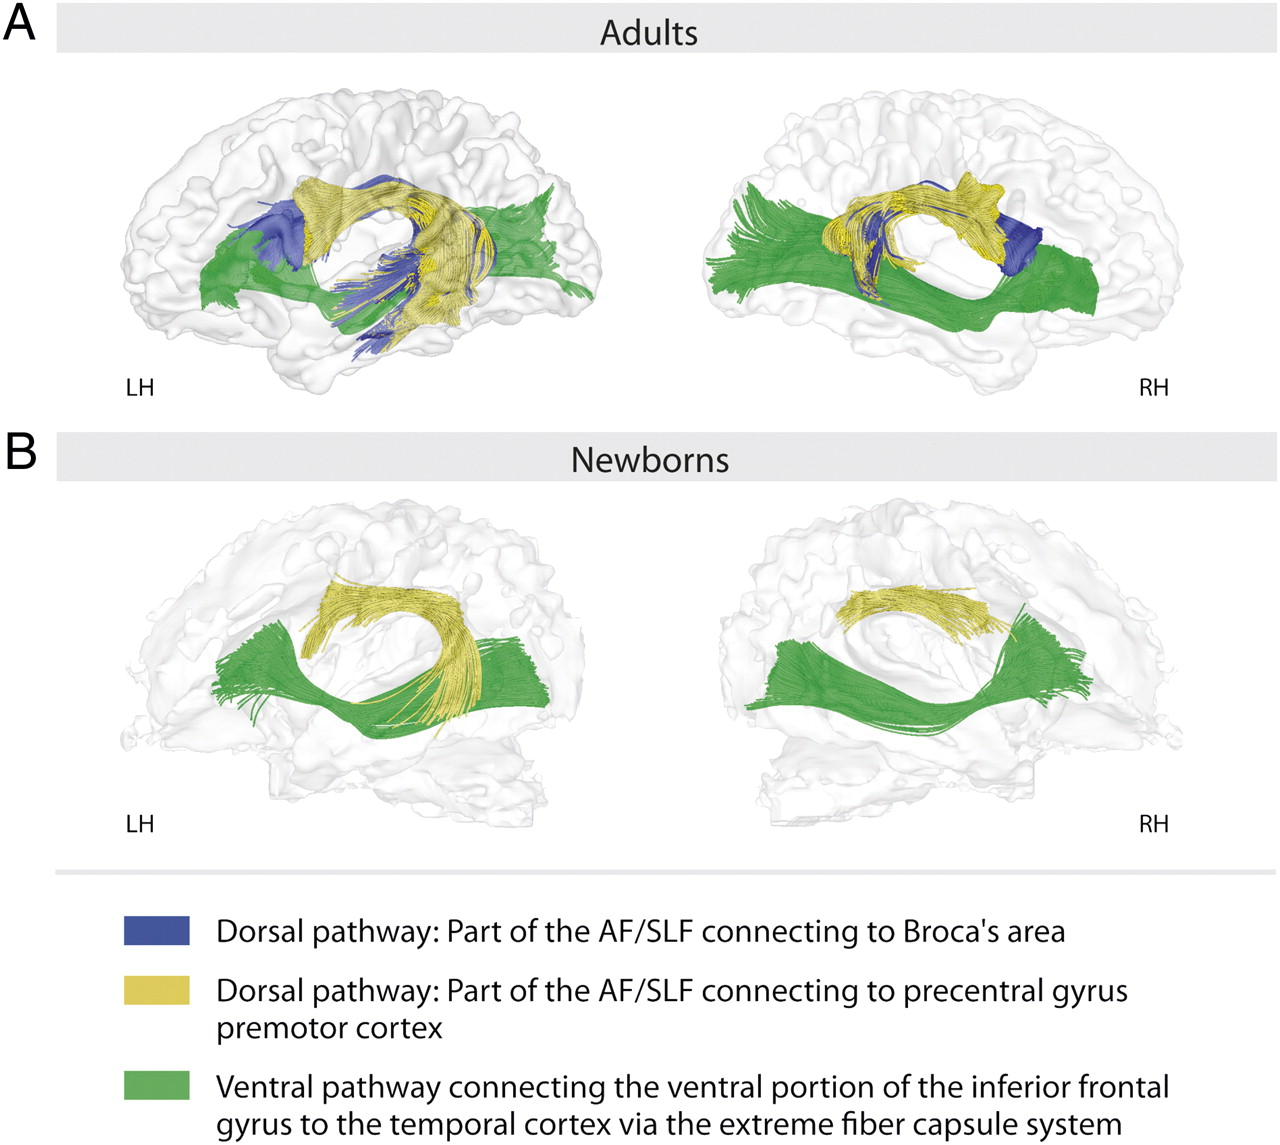
\includegraphics[width=1\textwidth]{Perani(2011)3}
	\caption[Perani(2011)3]{Perani(2011)对比了婴儿和成人听觉中枢的情况,发现婴儿颞叶到额叶见的联系只是初步建立,还不完善,由此推断新生儿只是听声音,但并不明白其含义.}
	\labfig{Perani(2011)3}
\end{figure}

上面这个系列实验是在实验室中通过严格的控制得出的结论,事实上,并不是只有在实验室中的实验才是科学实验,重要的是科学研究的思想。我们先简要说说\textbf{科学研究的思想},随后看看非实验室的研究可以怎样的出科学的结论.

\subsection{科学研究的思想与目标}

\begin{description}
    \item[1.系统的理论框架]
    只有有了系统的理论支持,收集数据才不是盲目的,上述实验中如果不是有Chomsky的理论支持,我们不会新生儿的语言获得情况有所兴趣,如果不是因为有FMRI研究技术的发展,我们不会想到用多功能核磁对新生儿进行研究.毕竟,一个刚出生两天的小婴儿,要其主观报告或者用其行为指标来反应其是否对语言有反应是不可能的.研究不是没有目的收集数据,而是有一定的理论支持,有一定的研究目的;
    \item[2.控制机制]
    主要是说的对无关变量进行控制,这一点和第三条一起说比较方便;
    \item[3.对象之间的因果关系]
    因果关系是心理学研究中最想得到的,想要做到为点需要有严格的控制.最理想的情况是研究者操控自变量在不同水平,并且控制无关变量,再对因变量进行观测,这样获得因变量观测值的差异就是由研究者在实验中让被试产生的,就可以很肯定的说是由自变量的变化导致的.关于这点我们还要再以后自变量的分类上谈,但此处要留个印象:最严格的因果关系是建立在实验中研究者人为造成的使被试形成的差异,比如上实验中输入的语料类型让婴儿由研究者的操作而导致的它们语言加工产生差异,这种差异是在实验室内产生的,是研究者明明白白控制了的,动因明确的.有些被试间的差异不是由研究者引起的,造成这个差异的原因也千奇百怪不得已而知,因此这类自变量往往不能得出严格的因果关系,比如说性别.因为行为学实验个体差异的关系,因此研究者通常用被试内设计,也就是一个被试要接受所有的处理,这样可以有效分离出被试间个体差异,这点我们后面要细谈,此处提及只是因为上实验(Peranti,2011)用的就是被试内实验设计,每个婴儿都听了这三段音频.
\end{description}


接下来我们以“对儿童说谎行为的研究”谈谈\textbf{科学研究目标}:

\begin{description}
    \item[1.描述]:如观察儿童说谎行为的各种不同表现形式、说谎的频率;
    \item[2.理解]:了解儿童说谎的原因(是否为了逃避批评或惩罚、或者为了获得某种利益?).我们知道儿童想要说谎必须有一定的认知机制,说谎不是一个简单的事情, 要有一定的认知能力才能说谎.要知道别人对问题是怎么想的,考虑别人怎么看问题才能说出来看起来比较严密的谎言,认知能力还没成熟的孩子说的谎在成年人看起来往往是可笑的;
    \item[3.预测]:什么样的家庭或学校环境下,什么年龄儿童可能出现说谎行为;
    \item[4.控制]:如果已经知道孩子在青春期喜欢说谎,并且这个现象不利于孩子的发展,那是否可以有合理的控制机制让说谎情况降到最低呢?
\end{description}


\subsection{心理学研究的途径}

下一步,我们继续讨论\textbf{心理学研究的途径},此处不会详细论述某种研究手段,想向各位传达的信息是,不是只有典型的实验研究才是研究,别的研究手段尽管没有对实验条件进行严格的控制,但这些手段都是科学的,都是为了一定的研究目的服务,也会进一步深入问题提供一个基础.额外想提醒的是,研究手段和研究目的紧密相关,有些现象没法用实验的手段,这点我们也放到后面的实验设计中谈.

\textbf{1.观察}

观察法指的是在自然状况下收集数据,描述某种现象包括自然现象,包括自然观察,问卷调查,个案研究.前面我们提到了儿童一岁半左右一个很有趣的词汇暴增现象——\textbf{词汇爆炸(vocabulary spurt)}.Bloom(1985)首先在国外儿童中发现了这个现象,那么中国儿童是否也存在这个现象呢?这就有赖于对汉语母语儿童的观察,我国学者确实发现在汉语母语儿童身上也发现了相同的现象(Li, 2007),下面介绍一下他们的研究.我们没法对6-7个月的儿童进行控制,让他们主观报告自己会说的词汇,因此只能让家长填写词汇问卷,判断哪些词是自己孩子说过的.这个词表数目还挺多的,让一个家长做完整个词表会造成较大的疲劳效应,因此实验中也匹配了一些“平行家长”,不过这都是控制机制,在此我不打算具体介绍.总之,在\reffig{Li(2007)}中我们确实看到,在18个月左右时,确实存在一个词汇量剧增的时间点.

这个实验中,我们不是被动的收集数据,而是有着某种特殊目的收集儿童的词汇量,并且这个实验结果得到了一个漂亮的结果.可见,描述性实验也失为一种有用的科学实验

\begin{figure}
    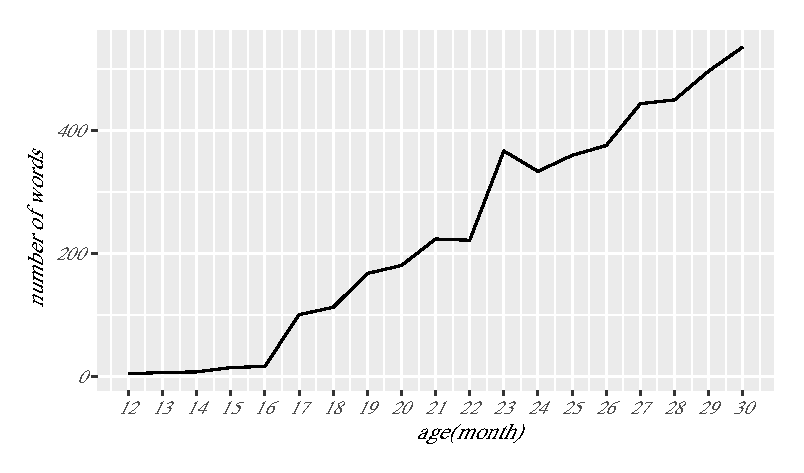
\includegraphics[width=0.8\textwidth]{Li(2007)}
    \caption{Li(2007)对12到30个月的汉语母语儿童进行了词汇量的追踪,结果发现了他们身上也存在词汇爆炸(vocabulary spurt)现象}
    \labfig{Li(2007)}
\end{figure}

\textbf{2.相关研究}
相关研究对两种现象(变量)之间的关系感兴趣,例如:吸烟与肺癌之间的关系.但是没法指因两个变量间引起与被引起的方向(到底吸烟引起肺癌,还是有肺癌基因的人倾向于吸烟不能从显著的相关中推论)

在对儿童语言发展的研究中,我们感兴趣的是孩子抚养人(特别是母亲)的语言使用清空对孩子会有什么样的影响,具体来说,父母寡言是否孩子也会寡言?父母受教育程度高是否导致孩子更喜欢说话?处于伦理道德的限制,我们只能记录孩子和父母的情况,不能对上述两个因素进行严格控制.

这个问题一直不能好好解决,因为要对一段录音中词语数进行统计是相当困难、工作量巨大的事情.不过LENA技术的出现让这种困境得以摆脱.这个程序可以识别婴儿的声音中的语言成分,并把一些非言语部分分离出去,比如哭声、吃东西的声音;它还可以分辨不同人的声音,这样也可以家长的说话情况.

这个实验的结果如\reffig{LENA}所示,我们能非常清楚地看到,父母地寡言和多言确实影响了孩子的与发展,
 
\begin{figure*}
    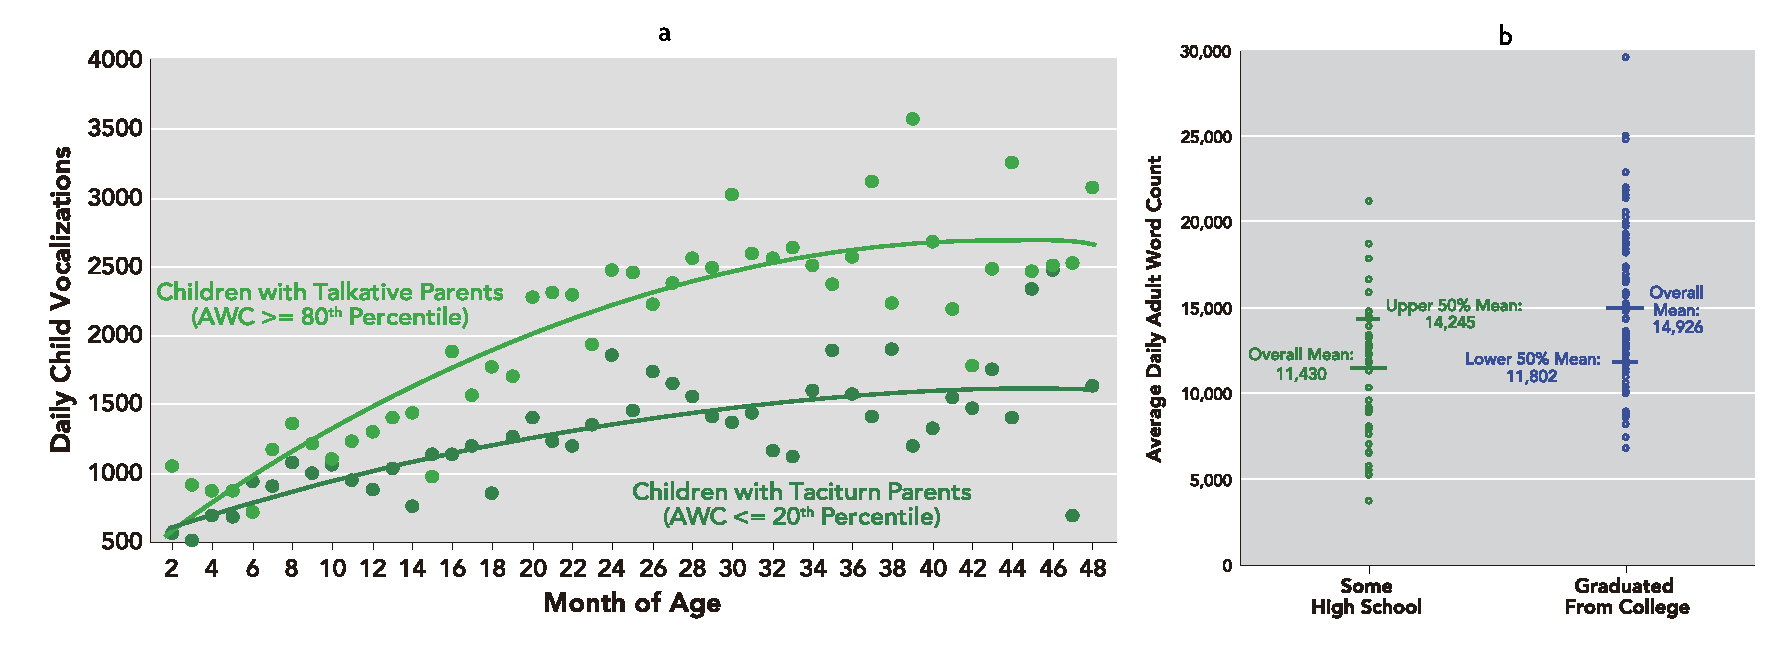
\includegraphics{LENA}
    \caption{用LENA研究父母多言寡言与受教育程度与孩子语言发展情况,结果发现这二者都和孩子的词汇发展成正相关}
    \labfig{LENA}
\end{figure*} 
 
\textbf{3.实验研究}

以Hagoort(2004)的一个研究为例看看他精细的设计.我们已经知道语义违反\sidenote{语义违反(semantic violation),指的是合乎语法要求却不符合词语的意义,如“这本书很咸”,从句法来看这句话是正确的,但是“咸”这个形容词不能修饰不是食物的名词,因此此处属于语义违反句子}会引起N400.还有一类句子错误,虽然语法、语义上都是正确的,但是和我们关于这个世界的认识是相违背的,比如“中国国家主席是位女士”.上述的两类错误涉及两种句子理解过程,一个是语义理解,一个是世界知识理解,以往人们认为这是两个独立的过程.Hagoort指出实际上这两种过程的区别不太好分开,因为很多词语都是不止有一个意思,多义词在特定语境中是什么意思要用世界知识来判断,进而Hagoort判断,世界知识违反(world knowledge violation)也会引起N400.

\begin{marginfigure}
    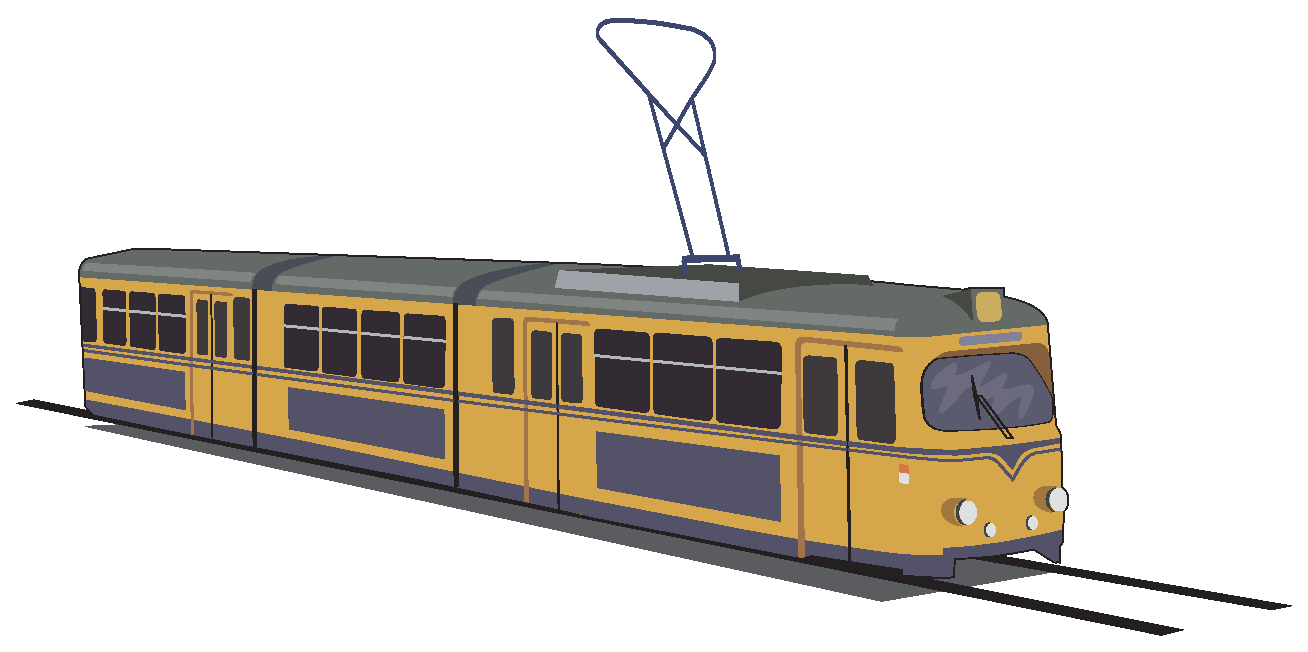
\includegraphics{dutch_train}
    \caption{荷兰火车的配色,实际上的车型并非如此}
    \labfig{dutch_train}
\end{marginfigure}

实验的材料(见\reffig{Hagoort(2004)}中的文字)经过了精心的设计,Hagoort给世界知识违反、语义违反、正确句子下了三个操作定义,这里用了一个非常有意思的操作定义来表示世界知识违反:实验的被试都是荷兰人,荷兰的火车都是黄色为主色调的(配色类似\reffig{dutch_train}),因此“The dutch trans are white”显然不符合荷兰人心中存在的对火车的知识.结果非常证实了Hagoort的猜想,在\reffig{Hagoort(2004)}可以清楚地看到,正确句子没有引起N400,而语义违反和世界知识违反都引起了N400.

\begin{kaobox}[frametitle=问题:如果这个实验只保留世界知识违反和正常条件,可行吗?]
如果顺着这个实验的结果来推理,这么做是看起来是可行的:把这个实验结果上的语义违反条件去掉,世界知识违反也确实引起了N400.但是要注意,实验前研究者并不知道结果是什么.也就是说实验前的假设是:\\
(1)若世界知识违反可以引发N400,说明语义理解与世界知识理解是一个连续的过程;\\
(2)若世界知识违反没有引发N400,说明语义理解与世界知识违反是两个独立的过程.\\
如果没有语义违反条件,(1)的结论还是可以得出,但是(2)中似乎存在了点问题.因为实验结果不显著不一定是处理效应不存在,还可能是检验力低的问题.对于心理学实验,它的处理效应本身就不高,那些不太明显但是确确实实存在的现象才有研究和发掘的价值.因此处理效应的显著需要较高检验力,实验设计一定要尽力精准和敏感.但不是所有实验都可以做到那么精准,想要得到漂亮的结果不是一件容易的事.在本实验中,如果没有语义违反做对照,在世界知识违反不显著时,研究者没法区分这是由实验不敏感导至的,还是由处理效应不存在导致的.因为语义违反已经被无数实验证明一定会引起N400,所以加上语义违反这个条件,就可以对实验的敏感性进行检验.这样(2)就可以拆分为以下两个假设:\\
(1)若世界知识违反没有引起N400,语义违反没有引起N400,则说明实验不够敏感,需要重新设计实验,处理效应是否存在有待继续检验;\\
(2)若世界知识违反没有引起N400,语义违反引起N400,则说明世界知识范围确实不会引起N400,世界知识违反和语义违反是两个独立的过程.
\end{kaobox}

\begin{figure}
    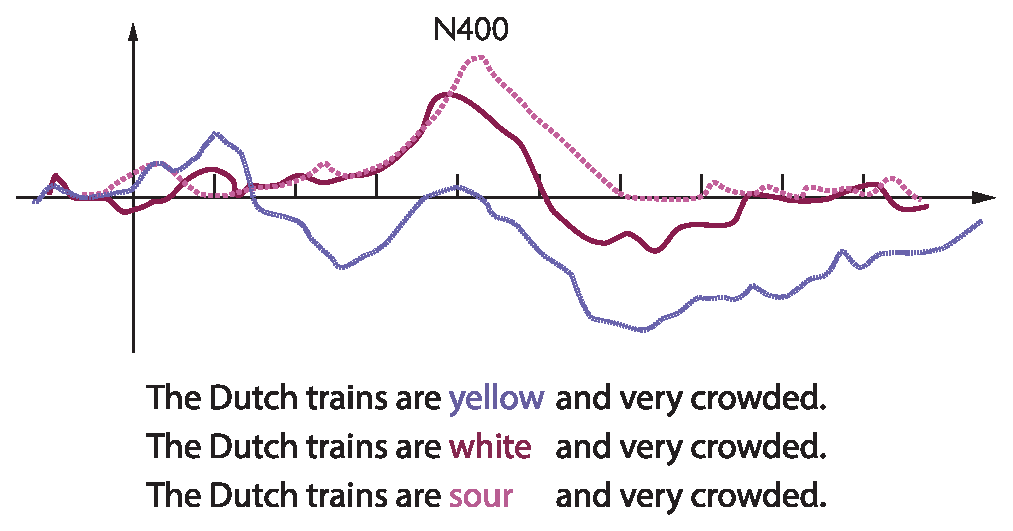
\includegraphics[width=1\textwidth]{Hagoort(2004)}
    \caption[Hagoort(2004)]{Hagoort(2004)给被试看三个句子并记录其脑电,发现世界知识违反的句子也会引起N400,进而说明了语义理解与世界知识理解是一个整体而不可以分割的过程.}
    \labfig{Hagoort(2004)}
\end{figure}

分析一下这个实验为什么是一个好实验.首先在自变量研究者控制了关键词的不同,在无关变量的控制上,除了关键词以外的句子都一摸一样,这样就排除了由于文字本身难度、熟悉度、使用频率带来的无关变异.实验设计上,采用被试内实验设计,每个被试都读了这三个句子,控制了所有的被试间的差异.这样总得来看,操作定义下得很精准、无关变量控制得也很巧妙,是一个值得我们学习的非常典型的实验设计.
%---------------------------------心理学实验设计基本问题
\section{心理学实验设计基本问题}

从上面的实验可以看到,\textbf{心理学实验的特点}是:

(1)影响因素多;(2)因素之间相互关联;(3)无关变量的混淆

研究者在操纵和改变自变量时候,有大量无关变量,有这么多复杂的因素需要控制,行为实验中最复杂的因素,这也是以人研究对象的实验的难点.当然我们也非常自豪地说,这是心理学家最擅长的.

我们接下来讨论什么是\textbf{实验设计}.广义的实验设计涉及的内容比较广泛,此处不予以介绍,我们看看狭义的、典型意义的实验设计要做什么.狭义的实验设计就是做好实验的计划方案、统计分析方案,就像盖房子需要一个蓝图,我们不能在盖房子前什么规划都不做就直接去盖,同样我们也不能没有计划就去进行一个实验.实验之前要做一个详细的规划,这非常重要.如果这个方案没有做好,之后便很难纠正.

\textbf{实验设计的主要目标}有三点,首先,要回答感兴趣的理论问题;其次,要获得更加丰富的信息;最后,要提高的敏感性.我们分别来看看这些目标的具体含义:

\begin{description}
	\item[1.回答感兴趣的理论问题] 
	~\
	前面已经提到了,我们感兴趣的问题是人类心理现象的规律性问题,也是对人类行为和心理现象产生的动因感兴趣.所以首先我们要建立变量之间的关系,在实验中操纵或改变一个或多个变量,并观察其对行为的影响,记录下因变量的观测指标的变化情况.
	
	但是影响某个心理或行为的因素不只有我们感兴趣的自变量那么简单,我们的想法是让不同被试仅仅在自变量上有所不同,并且这个不同是由研究者操纵的,这样结果就确定是由自变量引起的.但由于实验对象的特殊性,我们很难保重不同人在进行实验前是完全相等的,所以我们还要对那些对因变量也产生影响,但是不是为研究者所感兴趣的变量进行控制,也就是要控制无关变量,减小或控制其对因变量影响.
	
	最后,选用复杂的统计方法,在同样的数据量中得到更多有意义的信息.
	
	\item[2.更加丰富的信息]
	~\
	首先,可以选用更好的实验设计的种类,比如在多因素设计中,除了主效应,还有交互作用,而交互作用往往可以提供一些非常有用的信息.在研究中,不同因素间往往存在相互影响,忽略一个因素而研究另一个因素时,难以看到真实的结果,这就是单因素实验设计的局限.
	
	其次,可以选用丰富的因变量,这个等下举个例子说明.
	
	最后,正确选择一些复杂的统计
	
	\begin{kaobox}[frametitle=多因素实验设计的优点]
		~\
		(1)可以同时估计两个或多个实验处理的效应,可以估价实验处理之间的交互作用
		
		(2)因素实验设计可以对数据资源进行更加有效的利用,使同样数量的数据给出丰富的信息
		
		但是要注意的是,多因素实验设计的统计和解释可能会比较复杂,特别是对于一个高次的交互作用,很难解释其意义;并且,过多因素的实验设计可能设计时觉得还挺漂亮的,但是实际做出来交互作用都不显著.这提醒我们研究一个问题的时候要先深入研究该领域,,当有足够了理论支持多因素实验的交互作用显著时,多因素实验设计才可能成功.
	\end{kaobox}

	\item[3.提高实验的敏感性] 
		~\
		前面我们已经提到,处理不显著的时候,可能真的是处理效应不存在,也可能是实验设计不够敏感,我们要尽量减小后一种的可能性.不过大多时候如果处理效应不显著,我们并不能将这两者区分开来.
	
\end{description}



%记得整理一下这个实验=-= 还要自己画图嘤嘤嘤

%舒华(1996)的五张图
%字的类型和年级交互作用
\begin{marginfigure}
	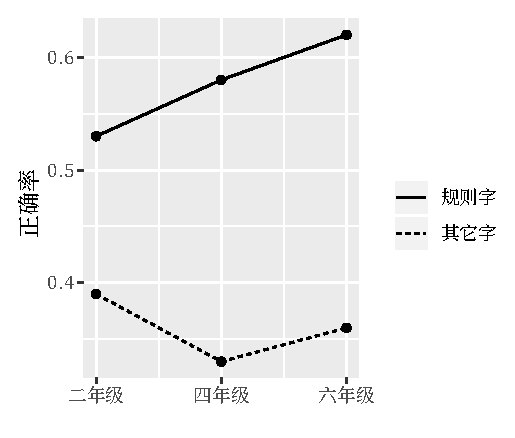
\includegraphics{shu(1996)_grade_type}
	\caption{字的类型$\times$年级}
	\labfig{shu(1996)t_g}
\end{marginfigure}

%字的类型和熟悉性交互作用
\begin{marginfigure}
	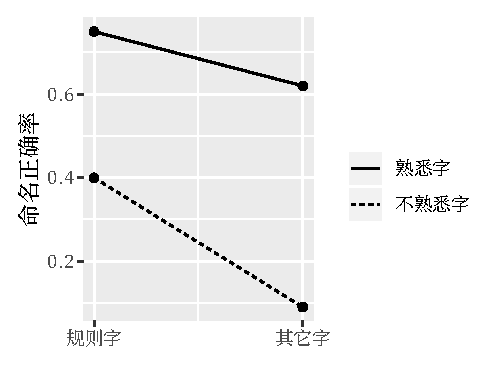
\includegraphics{shu(1996)_type_familiarity}
	\caption{字的类型$\times$熟悉性}
	\labfig{shu(1996)t_f}
\end{marginfigure}

%能力/熟悉性/类型三次交互作用图(重要! 好好解释)
\begin{marginfigure}
	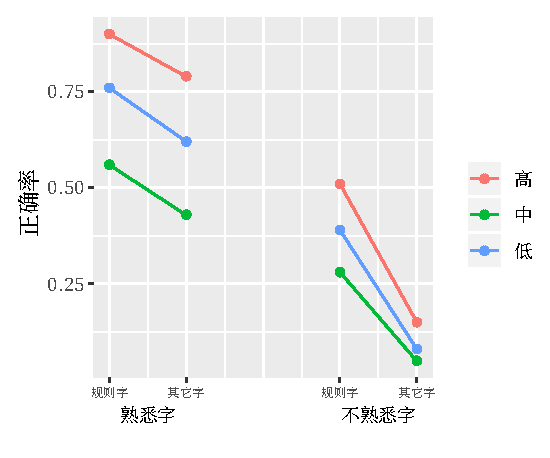
\includegraphics{shu(1996)_familiarity_type_capicity}
	\caption{能力$\times$熟悉性$\times$字的类型}
	\labfig{shu(1996)_t_f}
\end{marginfigure}

%错误分析
\begin{marginfigure}
	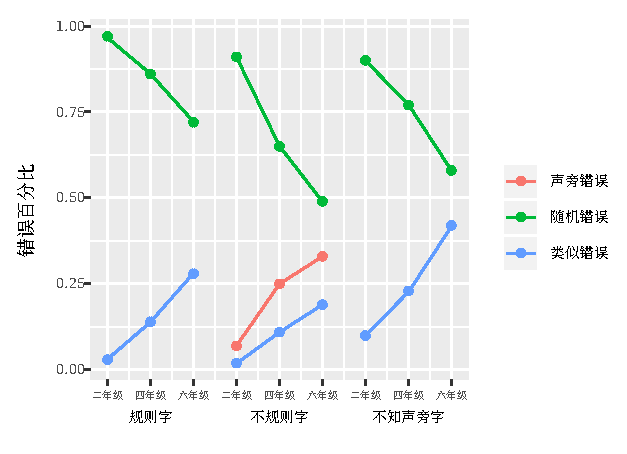
\includegraphics{shu(1996)false}
	\caption{儿童在各类字读音中犯不同类型错误占总错误的百分比}
	\labfig{shu(1996)_false}
\end{marginfigure}


%读音错误分析
\begin{marginfigure}
	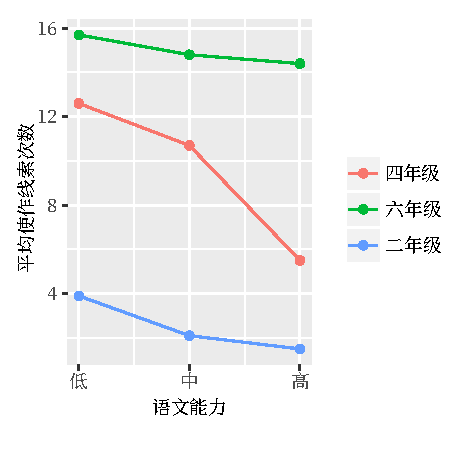
\includegraphics{shu(1996)_grade_capicity}
	\caption{儿童读音中使作线索的平均次数}
	\labfig{shu(1996)_cue}
\end{marginfigure}

舒华(1996)的一项研究中,对孩子读汉字的过程进行研究,特别是不熟悉的汉字.研究者想看到孩子读汉字能力的发展.实验中有一个非常漂亮的三次交互作用,揭示了一下有价值的信息.

这是一个3(年级)$\times$3(语文能力)$\times$2(字的熟悉性)$\times$3(字的类型)的四因素混合设计,其中字的熟悉性和字的类型是被试内变量,语文能力和年级是被试间变量.实验材料是60个单个形声字组成的卷子,所有的字都选自小学语文课本,每个年级的卷中包括30个熟悉的字和30个不有不同的字.熟悉字指学生在课本中已经学过的字,不熟悉字指学生在课本中还未学过的字,例如四年级卷子中的熟悉字选自第五、六册语文课本(三年级用书)后面的生字表,不熟悉字选自第九、十册语文课本(五年级用书)后面的生字表.每种熟悉度的字中有10个规则字,即字的声旁本身是一个儿童熟悉的汉字,且声旁的读音与字的读音相同,如“绘”;10个不规则字,即字的声旁是一个儿童熟悉的汉字,但声旁的读音与字的读音不相同,如“略”;和10个不知声旁的字,即字的声旁不是一个独立的汉字,其读音是一般人所不熟悉的,如“忱”,它的声旁“冘”的读音是“yin2”.不同熟悉度和不同类型的字的笔划数是经过匹配的,平均笔划数为10.实验是在三个自然班中集体进行的,每个学生接受相应年级的卷子,并按要求用拼音给出30个熟悉字和30个不熟悉字的读音,对写不出准确拼音的字,可以写一个与它同音的熟字代替. 

上述几个自变量比较难操作的是熟悉性.熟悉是最熟悉、全部都认识的吗?不熟悉、一定不认识的吗?这样做的话会出现天花板和地板效应,也就是熟悉的字成绩为100\%,不熟悉的字成绩为0.比较好的实验设计是,熟悉是比较熟悉,但也不是百分之百熟悉;不熟悉是相对不熟悉,也不是0.额外,上面提到,不同年级的材料间有一定的重叠这样使用的汉字数量比较少,这就减少了由汉字本身特点带来的无关变异.最后二四六年级的儿童匹配到的熟悉和不熟悉汉字的来源是:

\begin{figure}[hb]
	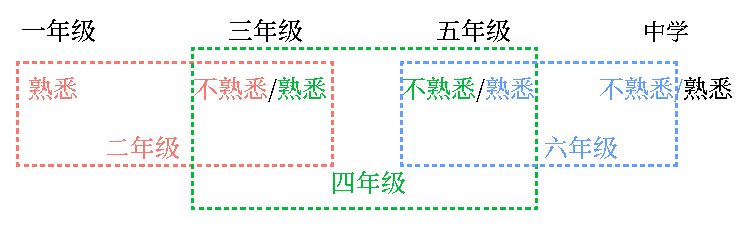
\includegraphics{shu(1996)_meterial}
	%\caption{舒华(1996)对二四六年级儿童熟悉字和不熟悉字的定义}
	\labfig{shu(1996)_meterial}
\end{figure}

年级和字的类型的交互作用显著(见\reffig{},规则字随着年龄增长,不规则字差不多,使用这个规则有一个学习过程

字的类型和熟悉性的交互作用显著,不规则的字更倾向于推理

语文能力三次交互作用显著,不熟悉的字中

对错误的分析中,三类
随机错误三类错误都下降
不规则字声旁错误增加
类似错误也是增加的
儿童对汉字的认知在发展,光读声旁很可能读错,所以在家族中找一个字

使用线索的次数,四年级有一个较大的发展

正确率由前侧,50\%正确率有较大变异

%-----------------------------------------------------------------
想要达到实验设计的目的主要通过以下三种手段:
\begin{description}
	\item[1.加大处理效应]
	有的时候增大处理效应不是一个很好的方法,因为处理效应太大了会没有意义.比如我想研究人的数学能力的发展,我选取3岁、15岁、60岁的人,可是我在实验前就已经知道60岁的人数学能力大于15岁的人大于3岁的人,这就没有研究的必要了.心理学的效应往往是日常生活中本身不太明显,以至于人们一般看不到这个现象,我们的研究就是要发现这个微弱的效应,并说明其探讨其存在意义.
	
	\item[2.减小误差]
	以方差分析为例,方差分析最后判断是否显著构成了一个$F$分布:
	$$
	F=\frac{MS_{effect}}{MS_{error}}
	$$
	
	实验的目的就是想让$F$达到显著水平,也就是$F$越大越好,上面已经否定让分子无限变大的可能性,那么分母是不是可以尽量控制让其减小呢?答案是肯定的,控制实验误差使其很小是实验设计的中心问题.
	
	\begin{kaobox}[frametitle=通过实验设计减小误差的方法]
		(1)区组、拉丁方实验设计\\
		(2)混合、被室内实验设计\\
		(3)嵌套、协方差实验设计
	\end{kaobox}
	
	\item[3.增加被试]简单要地说,在心理实验中,不管效应值多小,只要增加足够的被试量,总能达到接受备择假设的结果.增加样本容量意味着成本的,在有些心理学实验中这很困难,因此要注重别的提高实验敏感兴的方法.
\end{description}


统计在实验中的重要性

汉语阅读障碍儿童的认知缺陷 
Age reading Syslexia control
什么东西导致了阅读障碍?

语素意识、语音意识、命名速度 口语词汇(考察基本认知能力)——描述性
阅读障碍的孩子最基本的认知能力有关

相关

但是不能得到因果
1)追踪
2)训练

我们再来看两个研究,第一个研究室Eron(1972)非常著名的研究美国儿童看暴力电视和攻击性见关系的研究,一个是Lin(2011)对汉语阅读障碍儿童的追踪研究.

基于相关可以得到因果吗?
小学生对暴力电视的偏爱和攻击性Eron(1960)

之前的研究的表明,学校中表现出阅读障碍的孩子主要是三个基本认知能力不太好,分别是语音意识、语素意识和快速命名.这说明阅读障碍的孩子不是由于智力低,问题出在某些生理层面.孩子进入小学后再发现他们的阅读能力有障碍,会导致他们所有学科都不能好好发展,对于学龄儿童的干预也不如学前那么有效,因此研究者们想找到在学前可以预测上学后阅读障碍的指标,这样在学前对他们进行人为干预,哪种认知能力差就进行专门训练.

Lin(2011)发表一个6年的纵向研究,追踪了261名汉语孩子的基本认知能力的发展,用混合增长模型将他们分成四个亚类型:

\begin{itemize}
	\item \textbf{typical}:阅读能力正常发展的孩子
	\item \textbf{catch-up}:一开始基本认知能力比较差,但而后显示出正常的阅读能力的孩子
	\item \textbf{literacy-related-cognitive-delay}:在语音意识、语速意识、快速命名上表现较差的孩子,这些基本认知能力也导致他们的汉字识别量很低
	\item \textbf{language-delay}:所有的认知任务中都发展的相对较慢的孩子
\end{itemize}

结果(见\reffig{Lin(2011)})可以看到,正常发展的孩子(紫色)各项认知能力发展都很好;后来居上的孩子(红色)有一些能力在学前发展不太好,但是上学后有较好的发展;剩下的两组孩子(蓝色和绿色)的总体发展都不太好.额外,在8岁半的进行的文字识别和阅读流畅度测验中,后来居上的孩子\sidenote{研究者发现这些后来居上的孩子其实是因为在学前抚养者不爱说话,导致孩子接受了较少的语言刺激,尽管后来他们的各项基本认知能力有所恢复,但是在后面的两个和阅读和文字的任务中仍然表现的不够好}表现也不是特别好.这样研究者就得到了这样几个可以预测阅读障碍的指标——语音意识、语素意识、快速命名.

\begin{figure*}
	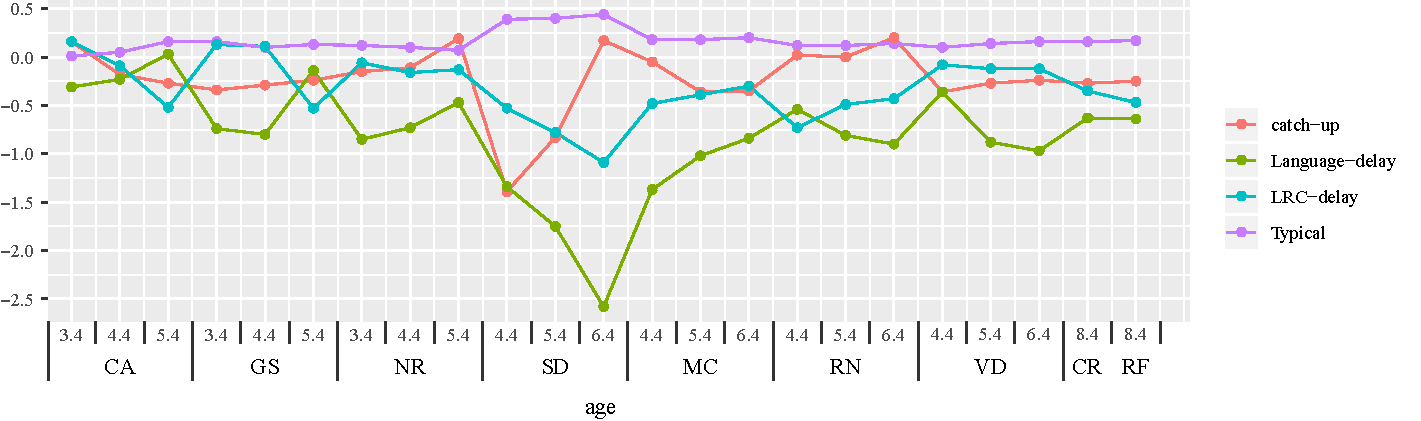
\includegraphics{Lin(2011)}
	\caption{Lin(2011)通过}
	\labfig{Lin(2011)}
\end{figure*}
	
上面的这个实验提到了一种叫混合增长模型的统计技术,我们简要介绍一下它.\reffig{Boscardin(2008)}是Boscardin(2008)的一项研究的结果,这个实验的数据分析就是用的这个模型.最大的图中,可以看到这个数学模型很好地把孩子分成两个亚类型,类型内的孩子比较接近,但是类型间的孩子相差较远;而且这些孩子中,有些孩子斜率相同,起点不同;有些孩子起点相同,斜率不同;也有可能起点不一样斜率也不一样.这就是用到复杂的统计,得到了非常丰富的信息.所以对于数学和统计学习一定要下尽全力,我们不仅要有最精细的实验设计,也要有最复杂的统计分析手段,这样才能做最好的研究,只是大多研究者醒悟的比较晚,若你现在还有心去学数学,那就立马去学吧!

\begin{figure*}
	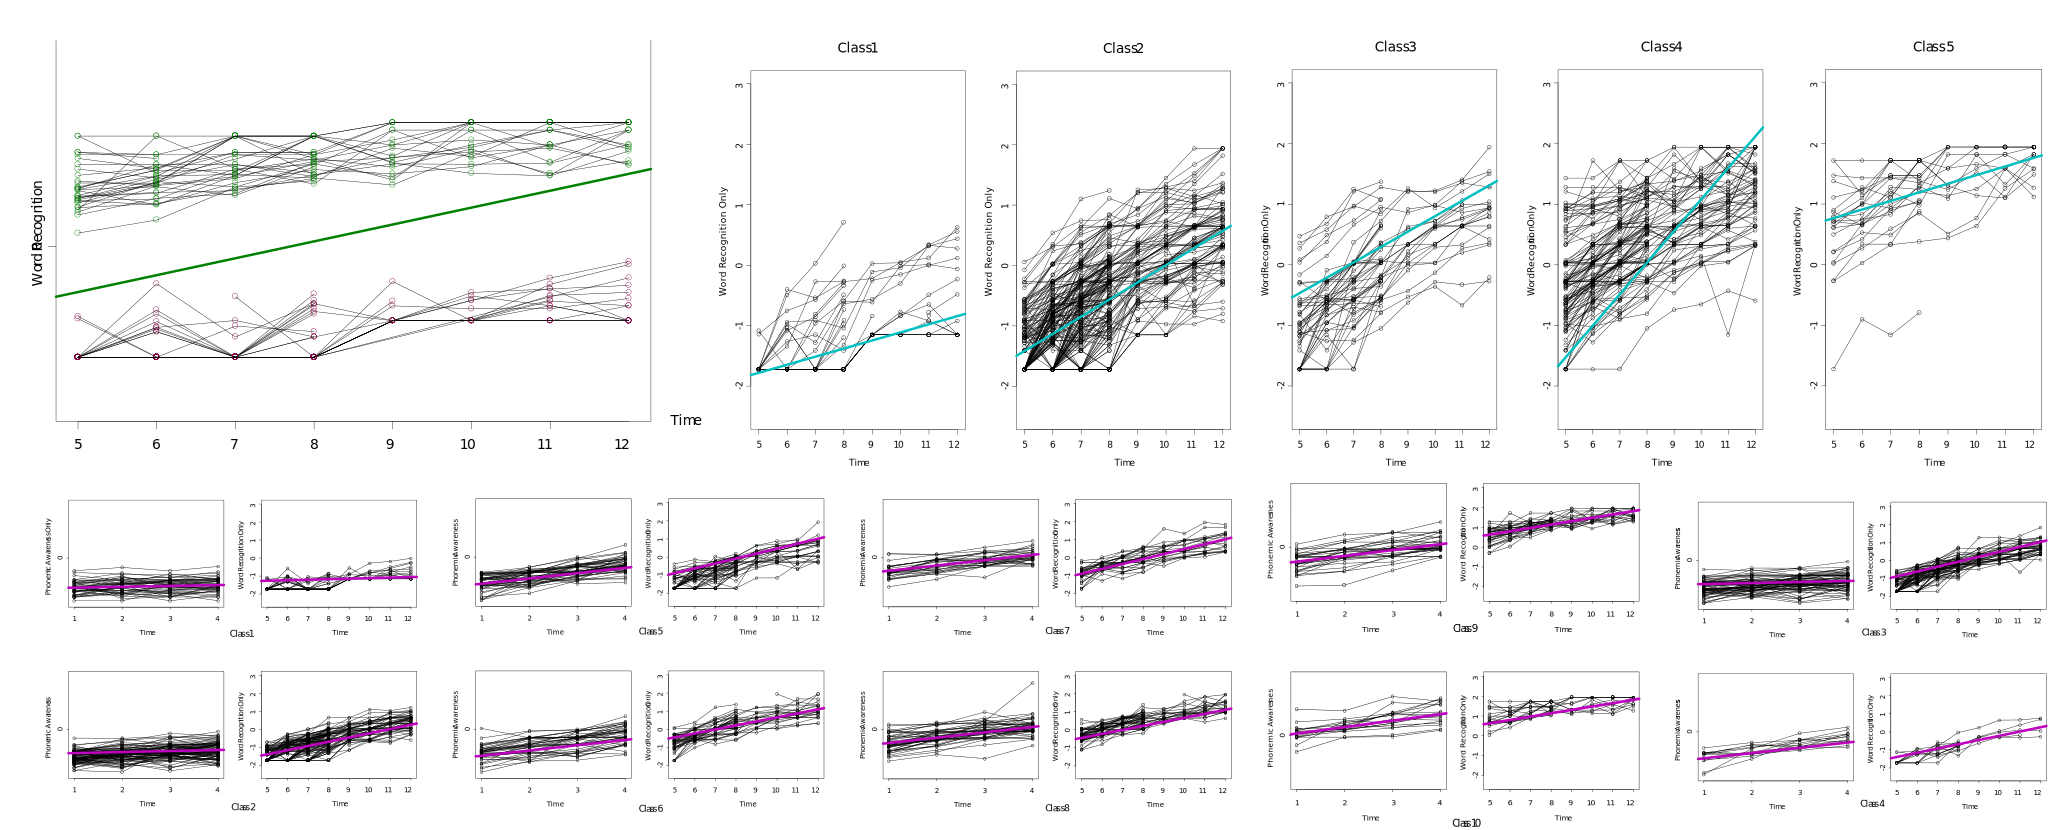
\includegraphics{Boscardin(2008)}
	\caption{Boscardin(2008)}
	\labfig{Boscardin(2008)}
\end{figure*}


前面介绍的部分实验用到了比较新的技术,一方面在工具上,针对于脑研究,像ERP/FMRI/眼动仪都是非常好的研究工具,它们帮助我们从更深层次探讨人脑的奥秘;另一方面,新的统计技术也让研究可以更精确的得出结果,包括已经写入大多课本的多重回归、路径分析、结构方程,也有上面提到的混合增长模型.不论这些手段多么的眼花缭乱,一定要注意,实质仍然是实验设计.比如下面这个实验,虽然仍然是行为学实验,不过实验设计非常有趣,非常漂亮地得到了结论.

\begin{marginfigure}
	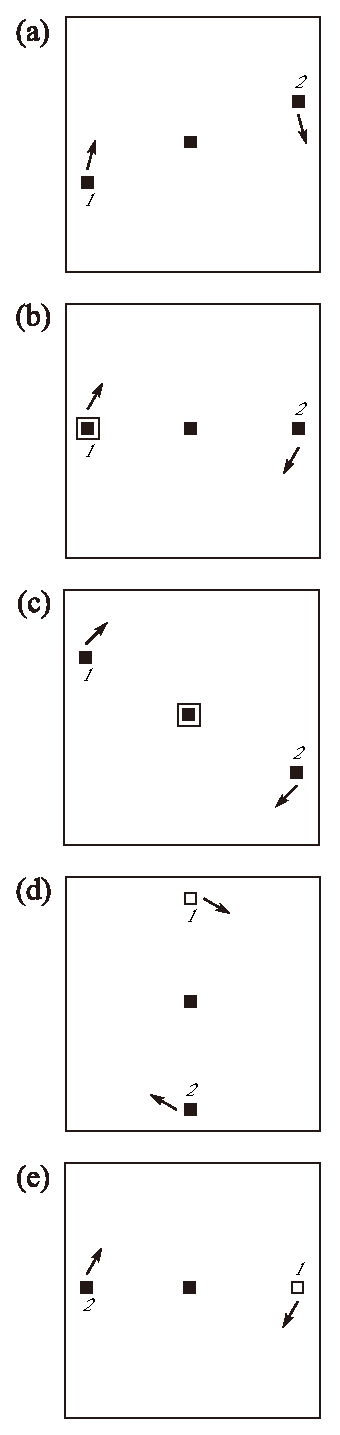
\includegraphics{Tipper(1991)}
	\caption{Tipper(1991)发现了基于物体的注意在返回抑制中相比基于空间的注意更具优势}
	\labfig{Tipper(1991)}
\end{marginfigure}

Tipper(1991)研究了注意中的返回抑制现象(inhibitation of return),所谓返回抑制,大体上是说对于我们注意过空间的某个区域,再次对其注意需要付出更多努力,在行为上的表现就是需要花费更多时间去重新注意.这点在学生看书时表现的很常见,在看完一本书后,我们好像有一种不知道哪里来的抗拒心理让我们不愿意复习.

Tipper想知道的是,我们到底是不愿意再注意注意过的物体,还是不愿意注意注意过的空间位置?若二者都存在抑制效应,哪种注意更占优势呢?\reffig{Tipper(1991)}是他的研究.初始状态a,有三个方块在视野中,方块1、方块2和中间的方块.1和2顺时针旋转到水平时(b),1闪烁,继续旋转到c后中间方块闪烁,然后等到旋转到e,此时1和2的位置和b中正好相反,然后1再次闪烁或者2闪烁,记录这次闪烁到按键间的反应时,发现被试更加难以注意1,说明了基于物体的注意在返回抑制中更有优势.

心理学研究的发展:
实验心理学:拥有严密的实验控制
教育与社会心理学:大样本+统计

复杂实验设计和多元统计的结合

推论统计——从样本推断到总体,不用
1有限的现象:可以观察到全体样本
2可以直接观察:DNA螺旋

统计假说:一种推论形式,可基于不完整的信息检验科学假说的真伪

方差分析的基本思想
对一组数据的描述:集中、离散
X1: 7 5 4 10 4
X2: 10 1 1 15 3
mean:6 6
range:4-10 1-15
var: 26 156

$$
	t=\frac{X_1-X_2}{S_P}
$$

变异是否存在?

施加处理:一致性变化(组内变化没变,组间有变)

随机分配被试来保证实验前被试同质

$$
	F=\frac{MS_{\text{处理效应}}}{MS_{\text{误差效应}}}
$$

下面应该是一个随机误差,所有处理效应要和误差效应相比,
%---------------------------------实验中变异的控制
\section{实验中变异的控制}
所谓变异(variance),就是对数据离散情况的衡量.和方差(variance)是一个词,不过实验中的变异含有三种变异

\textbf{1.使系统变异最大}
	\begin{itemize}
		\item 选取适当的自变量水平,使自变量水平的改变所引起的变异能在因变量中反映出来
		\item 选择对自变量的变化敏感的因变量
	\end{itemize}

这个实验中,一个是10,000条,一个是20,000条
因变量:容易形成正态分布
愿意买哪本?1010的数据,变化不敏感,变异小
%-----------------------------------------------------------------
\textbf{2.控制无关变异}
所有可能做自变量的因素均可能成为因素均可能成为无关变异的来源,无关变量是心理学、教育学、社会学研究中最棘手的问题之一.

上面大:例如研究两种教学条件对成绩的影响,实验选择两个班,但是可能两个班的学生能力不同,使得处理效应变异虚大
下面大:主要是被试带来的个体差异

这个实验中随机分配
指导语的描述一模一样,由不同文字引起的带走了

有五种控制无法变异的基本方法:

\begin{itemize}
	\item 随机化:随机分配被试
	\item 消除:i不是一个好方法,比如性别会影响,就只研究男性
	\item 匹配:基本上都是一样的
	\item 附加自变量
	\item 统计控制
\end{itemize}
%-----------------------------------------------------------------
\textbf{3.使误差变异最小}
误差指的是在实验中没有控制的变异:
主要来自于两个:处理单元内被试间的个体差异,我们知道这个是行为学实验中最主要的差异,
测量误差
尽量在实验设计中控制,实在控制不了的用统计控制 

实验设计的评价:内部效度(稳定性、控制无法变异)、外部效度
%---------------------------------假设检验的基本思想
\section{假设检验的基本思想}

要先说说统计的三大分布,这部分内容在概率中有详细论述,因此我也不打算说的很详细.

1. $\Gamma$函数

$$
\Gamma \left( x \right) =\int_0^{\infty}{e^{-t}t^{x-1}dt\left( x>0 \right)}
$$

性质:

\begin{align*}
    \text{(1) } & \Gamma \left( x+1 \right) =x\Gamma \left( x \right)  \qquad
    \Gamma \left( 1 \right) =1\Rightarrow \Gamma \left( n+1 \right) =n! \\
    \text{(2) } & \Gamma \left( \frac{1}{2} \right) =\sqrt{\pi}
\end{align*}


2.$\beta$函数
$$
\beta \left( x,y \right) =\int_0^1{t^{x-1}\left( 1-t \right) ^{y-1}dt\left( x>0,y>0 \right)}
$$
则有	 
$$
\beta \left( x,y \right) =\frac{\Gamma \left( x \right) \Gamma \left( y \right)}{\Gamma \left( x+y \right)}
$$

1.$\chi ^2$分布(Chi-Square Distribution)
$$
\text{设}X_1, X_2,..., X_n\,\,iid,\sim N\left( 0,1 \right) , \text{令}\chi _{n}^{2}=\sum_{i=1}^n{X_{i}^{2}}
$$

称$\chi _n^2$是自由度为$n$的$chi$方分布,其密度函数为 :
$$
f_n\left( x \right) =\frac{1}{\Gamma \left( \frac{1}{n} \right) 2^{\frac{n}{2}}}\cdot e^{-\frac{x}{2}}\cdot x^{\frac{n-2}{n}}\left( x>0 \right) 
$$

$chi$方分布有一个重要的性质:设$X_1\,\,,X_2$独立,$X_1\sim \chi _{m}^{2}, X\sim \chi _{n}^{2}$,则$X_1+X_2\sim \chi _{m+n}^{2}$ 

2.$t$分布
设$X\sim N\left( 0,1 \right) , Y\sim \chi _{n}^{2}$ ,且$X,Y$独立,于是

$$
t_n=\frac{X}{\sqrt{Y/n}}\left( \frac{N\left( 0,1 \right)}{\sqrt{\chi _{n}^{2}/n}} \right) 
$$

称t服从自由度为$n$的$t$分布,$t$分布的自由度与其分母的¥方自由度相等,其密度函数为: 
$$
f_n\left( t \right) =\frac{\Gamma \left( \frac{n+1}{2} \right)}{\sqrt{n}\pi \Gamma \left( \frac{n}{2} \right)}\left( 1+\frac{t^2}{n} \right) ^{-\frac{n+1}{2}}
$$

$t$分布图像如所示,可以看到$t$分布与正态分布在一起时,$t$分布的形态好像“尾巴非常重,头变轻”,故$t$分布有也被叫做heavy tail(重尾).由图像亦可知,$t$分布随着自由度的变大,“头上的鼓包”渐渐缩小,本来“繁重的尾巴”渐渐变轻,越来越朝着标准正态分布的图像靠近.

3.$F$分布

设$X\sim \chi _{m}^{2},Y\sim \chi _{n}^{2}$,且$X$与$Y$独立,令 ,称$F$为服从自由度$m,n$的$F$分布.
当$m=1$时
$$
F_{1,n}=\frac{\chi _{1}^{2}/1}{\chi _{n}^{2}/n}=\left( \frac{N\left( 0,1 \right)}{\sqrt{\chi _{n}^{2}/n}} \right) ^2=t_{n}^{2}
$$
故
$$
t_{n}^{2}\sim F_{1,n}
$$

F分布的基本假设

因变量观测值大体服从正态分布,如果数据不可能符合正态分布,就不能用F检验
 
变异的同质性:由随机分配保证,是一个最基本的假设,因为我们根本就不做前测,只做后测
	加实验处理只是变了组间变异,实验后的组间变异也反应了处理前的组内变异
 
 独立性:每一个观测值独立于其它观测值 


实验设计模型及其假设:变异的构成
一次观测就只有一个观察值,但是怎么知道这个观察值有哪些组成的?这个模型就是指导这件事,
如:
$$
Y_{ij}=\mu +\alpha_j + \varepsilon_{i(j)}
$$

$$
SS_{total}=SS_{within\_group}+SS_{between\_group}
$$



误差是一个平均数为0的随机变量,不是一个定向的变化


实验设计的基本过程:
1提出问题和假说的形成
问题特征:探索两个或多个变量间的关系
问题的可检验性:研究该问题的方法和手段已经解决或初步解决
Science 290 ,1582-1585(2000) 有意思的问题,在以前是没法做的,婴儿没法报告
问题所包含的变量是可以检验并可以操作化的(操作定义)
怎么操作世界知识违反操作化?非常精巧化
%---------------------------------实验中的变量
\section{实验中的变量}
变量的选择能否回答想解决的问题?
符合:1研究的理论假说/实验设计和统计的要求

\textbf{被试固有特性}:被试在实验前就有的,不太可能改变和操纵,通常分类
严格地来说,追踪的研究能得到严格的因果关系吗?
最严格的因果关系是操纵和改变自变量,引起心理或行为上的变化
有些情况下没有办法做这个
但是又没有办法做,已经是最好的了
通常在实验中还会加一个可以操控的,不会让自变量只有被试固有特性,

\textbf{被试的暂时特性}:心理学严重最丰富,最具特色的自变量.操纵外部刺激引起心理变化,不是完全外部,引起的心理变化正好是想研究的问题,但是比较难以操纵,需要找到非常好的操作定义.

可操作、可改变的
不可操作、不可改变的

自变量的数量:与问题、统计方法有关
水平的数量:动机的那个例子

主要意义次要次要意义,定SOA,43
主要意义一直维持激活,次要意义有一个上升下降的曲线


因变量:可以看到的
必须随着自变量的变化而变化
可以转化为数据

1)对自变量的变化最敏感:字典中
2)实验中选取的观测量应该可靠,得出稳定的结果
3)大体上正态分布,人的行为、生理大体上都符合正态分布,但是如果数据就不可能服从正态分布就不要用方差分析
4)可行性上考虑

Keenan(2001)自我面孔实别

无关变量

操作定义:变量必须用测量或操作它们的步骤来定义
用事物可观察、可测量的特征把研究变量具体化,它清楚地讲明与栽些现象独特联系的可观测的准则

意义:
1、对研究结果评价:同意研究结果必须先接受操作定义
2、有利于研究间交流:在前人基础上重复或修改实验
3、保障可重复性

获得方式:
1、使用现有信息:性别、教育程度、智力
2、操作创建一种形态:让被试进入实验后让其脑子发生变化,最重要
3、通过前测、评定、记录获得信息,如语义相关

Rosler(2001)

Loftus(1974)看相同的视频, 只是问题的词不同
The possible speed when the two cars
%---------------------------------实验的诚信问题
%\input{chapters/design/.tex}








%\setchapterpreamble[u]{\margintoc}
\chapter{单因素实验设计}
\labch{options}

\subsection{良好实验在统计上的体现}
以往在论述实验设计时,我们称随机区组设计和被试内可以带走使实验更加数来宝这样一个事实,但这只是描述性的话,没有数据的前后对比无法让人真的信服随机区组和被试内设计的好处.所以,现在要从数据上看到$F$怎样更容易显著.

所谓$F$更容易显著无非就是$F$更大了($F=MSA/MSE$),想让$F$变大有两个手段,让处理效应($MSA$)变大,或者让误差效应($MSE$)变小,这件事情在前面已经介绍过.我说过心理学家感兴趣的那些现象往往都不太大\sidenote{也可以说是效应量(effect size)总是不太大},而且人为加大处理效应有时没有什么意义.从实验设计的角度上,减小误差才是关键.

\begin{marginfigure}
	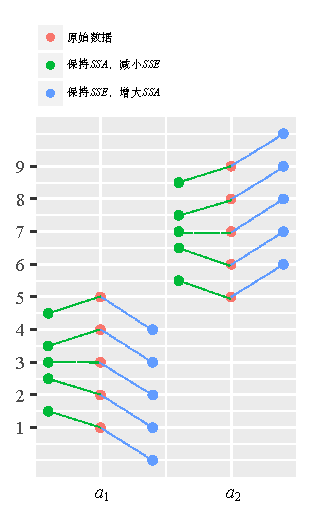
\includegraphics{SSA_SSE}
	\caption{红色是原始数据,蓝色代表组内误差不变,加大处理效应;绿色代表组间变异不变,改变组内误差}
	\labfig{SSA_SSE}
\end{marginfigure}

这就好比用天文望远镜观测外太空,我想发现人们不曾发现过的行星,我透过天文望远镜可以看到一些噪音——没有规律发亮的光点,但是那颗星星好像也在发光,我想鉴别这个星星是否真实存在,但是这件事情不是那么容易,因为星星发的光和噪音总是同时出现,故只有星星发出的光足够大,大到和周围的噪音是那么的与众不同,我再将这个星星是噪音有很大几率犯错,我才敢认定那是星星.我们清楚地知道,想要更加清楚地观察到星星无非有两种手段,其一是让星星在原有基础上多发电光;其二是让周围的噪音降低点.

方差分析模型中的$MSA$和$MSE$是相互独立的,它们俩可以独立地变化.随机误差指的是由随机因素导致数据在理想值周围随机晃动的偏差,它要是和处理不独立那就不能叫随机误差了.

\begin{kaobox}[frametitle=思考]
假定我们有一组分数,分别计算出$MSA$和$MSE$.\\
(1)我们可以改变$AS$\sidenote[*5][]{$AS$中A代表因素$A$的处理效应,$S$代表被试个体误差,具体是什么后面再说}分数,保持处理平均数恒定.即保持$MSA$不变而改变$MSE$.\\
(2)如果我们改变组平均数,处理组内分数关系不就,$MSA$会变化,而$MSE$不就.表明两个均方是独立变化的.



\end{kaobox}

我们看一组数据
\begin{align*}
    a_1:1, 2, 3, 4, 5\\
    a_2:5, 6, 7, 8, 9
\end{align*}

(1)调整原始数据,保持$SSA$不变,而$SSE$改变(减小$SSE$) (通常加大处理效应实现)

(2)调整原始数据,改变$SSA$不变(增大$SSA$),而$SSE$不变

我直接给出我的思路,\reffig{SSA_SSE}中红色是原始数据,它有两个水平,$a_1$的各个值围绕其均值3波动,$a_2$的各个值围绕其均值7波动.

绿色是我写的符合(1)的一组数据,可以看到红色数据$a_1$处理的每个数据都围绕着3波动,现在绿色的值在$a_1$内还是围绕3波动,但是数据间的距离更短了,它们显得更加紧密.虽然从组内均值上来看(3和7)两组数据的平均值之差不变,但是由于$a_1$的数据更集中于3,$a_2$的数据更集中于7,故实际上这样两组间的差异其实增大了.

蓝色是我写的符合(2)的一组数据,可以看到数据间的紧密程度不变,$a_1$整体向下移动,$a_2$整体向上移动,这样组间的差距被拉大.

原始数据方差分析结果是.

\begin{table}[h]
	\centering
	\caption{原始数据方差分析}
	\labtab{RAW_ANOVA}
	{
		\begin{tabular}{cccccc}
			\toprule
			变异来源 & $SS$ & $df$ & $MS$ & $F$ & $p$  \\
			\midrule
			组间变异 & 40.000 & 1.000 & 40.000 & 16.000 & 0.004  \\
			组内变异 & 20.000 & 8.000 & 2.500 &  &    \\
			\bottomrule
			% \addlinespace[1ex]
			% \multicolumn{6}{p{0.5\linewidth}}{\textit{Note.} Type I Sum of Squares} \\
		\end{tabular}
	}
\end{table}

\begin{margintable}
    \caption{保持$SSA$不变,减小$SSE$}
    \labtab{lower_SSE}
    \raggedright
    \begin{tabular}{cccccc}
        \hline
        $a_1$ & 1.5 & 2.5 & 3 & 3.5 & 4.5\\
        $a_2$ & 5.5 & 6.5 & 7 & 7.5 & 8.5\\
        \hline
    \end{tabular}
\end{margintable}

绿色数据见\vreftab{lower_SSE}.


其方差分析结果是,可以看到相比\vreftab{RAW_ANOVA}中的数据,处理效应没变,误差效应减小了,$F$值变大,$p$值减小.

\begin{table}[h]
	\centering
	\caption{绿色数据方差分析}
	\label{tab:aNOVA-Score}
	{
		\begin{tabular}{cccccc}
			\toprule
			变异来源 & $SS$ & $df$ & $MS$ & $F$ & $p$  \\
			\midrule
			组间变异 & 40.000 & 1.000 & 40.000 & 32.000 & $<$ .001  \\
			组内变异 & 10.000 & 8.000 & 1.250 &  &    \\
			\bottomrule
			% \addlinespace[1ex]
			% \multicolumn{6}{p{0.5\linewidth}}{\textit{Note.} Type III Sum of Squares} \\
		\end{tabular}
	}
\end{table}

\begin{margintable}
    \caption{保持$SSE$不变,增大$SSA$}
    \labtab{UPPER_SSA}
    \raggedright
    \begin{tabular}{cccccc}
        \hline
        $a_1$ & 1 & 1 & 2 & 3 & 4\\
        $a_2$ & 6 & 7 & 8 & 8 & 10\\
        \hline
    \end{tabular}
\end{margintable}

蓝色数据见\vreftab{UPPER_SSA}.

其方差分析结果是,可以看到相比\vreftab{RAW_ANOVA}中的数据,处理效应变大,组内误差减没变,$F$值变大,$p$值减小.

\begin{table}[h]
	\centering
	\caption{蓝色数据方差分析}
	\label{tab:aNOVA-Score}
	{
		\begin{tabular}{cccccc}
			\toprule
			变异来源 & $SS$ & $df$ & $MS$ & $F$ & $p$  \\
			\midrule
			组间变异 & 90.000 & 1.000 & 90.000 & 36.000 & $<$ .001  \\
			组内变异 & 20.000 & 8.000 & 2.500 &  &    \\
			\bottomrule
			% \addlinespace[1ex]
			% \multicolumn{6}{p{0.5\linewidth}}{\textit{Note.} Type III Sum of Squares} \\
		\end{tabular}
	}
\end{table}




\section{单因素完全随机实验设计}
\subsection{基本特点}

完全随机设计(completely randomized design)的假定是,由于被试是从总体中随机选取,处理也是随机分配给被试,那么被试间的差异也是随机、在统计上无差异的.

\begin{margintable}
	\centering
	\caption{单因素完全随机实验设计中被试的分配}
	\labtab{one_way_ANOVA_data}
	{
		\begin{tabular}{cccc}
			\toprule
			$a_1$ & $a_2$ & $a_3$ & $a_4$ \\
			\midrule
			$S_1$ & $S_2$ & $S_3$ & $S_4$ \\
			$S_5$ & $S_6$ & $S_7$ & $S_8$ \\
			$S_9$ & $S_{10}$ & $S_{11}$ & $S_{12}$ \\
			$S_{13}$ & $S_{14}$ & $S_{15}$ & $S_{16}$ \\
			\bottomrule
			% \addlinespace[1ex]
			% \multicolumn{6}{p{0.5\linewidth}}{\textit{Note.} Type III Sum of Squares} \\
		\end{tabular}
	}
\end{margintable}

单因素完全随机设计中分配被试的图解例子如\vreftab{one_way_ANOVA_data},
个因素$A$有4个水平,每个处理下有4个被试.完全随机设计是一种被试间设计,这意味着每一个被试只接受一种处理或处理的组合
\sidenote[*-5][]{处理的组合是多因素实验中会遇到的,后面遇到了再说}
,故对于本例而言需要16个被试.

对按下来要描述的模型的字母进行一下简要的说明:

(1)假设因素$A$有$p$个水平,用$\alpha _j$表示其第$j$个水平($1 \leq j \leq p$),也就是说$A$的水平分别是$\alpha _1,\cdots,\alpha _j,\cdots, \alpha _p$,

(2)$p$个处理下的被试数都相等,均为$n$个,用$i$表示每个处理下第$i$个被试($1 \leq i \leq n$)

(3)假设被试在没有施加处理的时候,无限次实验结果的平均数是$\mu$.该值是个理想值,其实意思是被试测量值在理论上的基线,不过这么说只是表达了概念.虽然说明了更加明确的定义不过可以充分的感受到,这个理论基线值是无法获得的,毕竟无限次是个极限,不是一个具体的数,所以$\mu$是个理论值.

(4)假设实验中的误差是$\varepsilon _{i\left(j\right)}$
\sidenote{关于为什么它的下标是带括号的现在不便解释.}
,其平均数为0,方差为$\sigma _e^2$,我们进一步假设它服从正态分布

(4)观察值$Y_{ij}$指第$j$个处理水平下,第$i$个被试的观测值

后现的章节因素多了会加入一些新字母和下标,和上述符号已经没有本质区别,故以后我不打算再介绍新符号了.

单因素完全随机设计的原假说是:多个处理水平上的总体平均数相等,即
$$
H_0: \mu _{.1}=\mu _{.2}=\cdots=\mu _{.p}
$$

或处理效应等于为0,即
$$
\alpha _j=0
$$


单因素完全随机实验设计模型
\begin{equation}
    Y_{ij}=\mu +\alpha _j+\varepsilon _{i\left( j \right)}
\end{equation}

其中:

\begin{tabular}{lcl}
    $Y_{ij}$ & - & 被试$i$在处理水平$j$上的分数 \\
    $\mu$ & - & 总体平均数 \\
    $\alpha _j$ & - & 水平$j$的处理效应 \\
    $\varepsilon_{i \left( j \right)}$ & - & 误差效应 \\
\end{tabular}



\subsection{实验设计与计算举例}

\subsubsection{研究的问题}
我想研究文章的生字密度对学生阅读理解的影响.我的假设是:阅读理解随着文章中生字密度的增加而下降。因此,该实验有一个自变量——生字密度,通过研究前人文献我感兴趣的是四种生字密度
(1)$5:1\left(a_1\right)$、
(2)$10:1\left(a_2\right)$、
(3)$15:1\left(a_3\right)$、
(4)$20:1\left(a_4\right)$
因变量是被试的阅读理解分数。实施实验时,我将32名被试随机分成四组,每组被试阅读一种生字密度的文章,并回答阅读理解测验中有关文章内容的问题。这是一个典型的单因素完全随机设计。虽然我不再检验实验中其他因素的影响,但实际上存在着诸多对因变量影响的无关变量,比如文章的长度、文章的主题熟悉性、文章类型等,还有被试的年龄、受教育程度、阅读能力等。这时,控制无关变量可做的工作之一是在选取四篇文章时,使它们在除生字密度以外的其他方面尽量匹配。

\subsubsection{新的计算模型的引入以及数据的计算}
我将引入一种新的计算模式,这种模式主要是为了手算.为了理解愿意,我们必须手算一次每种实验设计的简单数据,但是用统计教材上的算法根本无法实现一个较为精确的估算,其原因是,和方的计算公式选用:

$$
    SS =
        \sum\limits_{i=1}^{n}
        \left( 
            X_i -\bar{X} 
        \right)^2
$$

式子中$\bar{X}$很大可能是小数,且可能是循环小数,所以每次相减都会四舍五入,然后平方后进一步放大误差,这样算到最后误差不断累记.所以应当最后一步再做除法,把上面的式子改写一下:

\begin{align*}
SS= & \sum\limits_{i=1}^n{\left( X_i-\bar{X} \right) ^2}
\\
    & =\sum\limits_{i=1}^n{\left( X_{i}^{2}+\underset{\text{常数}}{\underbrace{\bar{X}^2}}-\underset{\text{常数}}{\underbrace{2\bar{X}}}X_i \right)}
\\
    & =\sum\limits_{i=1}^n{X_{i}^{2}}+n\bar{X}^2-\underset{2n\bar{X}^2}{\underbrace{2\bar{X}\sum\limits_{i=1}^n{X_i}}}
\\
    & =\sum\limits_{i=1}^n{X_{i}^{2}}-n\left( \frac{\sum\limits_{i=1}^n{X_i}}{n} \right) ^2
\\
    &= \underset{\text{离散+集中+可能个体差异}}{\underbrace{\sum\limits_{i=1}^n{X_{i}^{2}}}}-\underset{\text{集中}}{\underbrace{\frac{\left( \sum\limits_{i=1}^n{X_i} \right) ^2}{n}}}
\end{align*}

这样除法只进行了一次(上式“集中”那里算了一次除法,产生误差),其余的都是乘法和加法.那么在方差分析中,大量求$SS$,用这样的方法就可以利于手算,以便更好了解方差分析原理.


\textbf{1.计算表}

\begin{margintable}
	\centering
	\caption{单因素完全随机实验的$AS$表}
	\labtab{one_way_ANOVA_AS_TAB}
	{
		\begin{tabular}{cccccc}
			\toprule
    			     & $a_1$ &  $a_2$ &  $a_3$ &  $a_4$ & \\
    			     \midrule
                              & \cellcolor[rgb]{ .949,  .949,  .949}3 & \cellcolor[rgb]{ .949,  .949,  .949}4 & \cellcolor[rgb]{ .949,  .949,  .949}8 & \cellcolor[rgb]{ .949,  .949,  .949}9 &  \\
                              & \cellcolor[rgb]{ .949,  .949,  .949}6 & \cellcolor[rgb]{ .949,  .949,  .949}6 & \cellcolor[rgb]{ .949,  .949,  .949}9 & \cellcolor[rgb]{ .949,  .949,  .949}8 &  \\
                              & \cellcolor[rgb]{ .949,  .949,  .949}4 & \cellcolor[rgb]{ .949,  .949,  .949}4 & \cellcolor[rgb]{ .949,  .949,  .949}8 & \cellcolor[rgb]{ .949,  .949,  .949}8 &  \\
                              & \cellcolor[rgb]{ .949,  .949,  .949}3 & \cellcolor[rgb]{ .949,  .949,  .949}2 & \cellcolor[rgb]{ .949,  .949,  .949}7 & \cellcolor[rgb]{ .949,  .949,  .949}7 &  \\
                              & \cellcolor[rgb]{ .949,  .949,  .949}5 & \cellcolor[rgb]{ .949,  .949,  .949}4 & \cellcolor[rgb]{ .949,  .949,  .949}5 & \cellcolor[rgb]{ .949,  .949,  .949}12 &  \\
                              & \cellcolor[rgb]{ .949,  .949,  .949}7 & \cellcolor[rgb]{ .949,  .949,  .949}5 & \cellcolor[rgb]{ .949,  .949,  .949}6 & \cellcolor[rgb]{ .949,  .949,  .949}13 &  \\
                              & \cellcolor[rgb]{ .949,  .949,  .949}5 & \cellcolor[rgb]{ .949,  .949,  .949}3 & \cellcolor[rgb]{ .949,  .949,  .949}7 & \cellcolor[rgb]{ .949,  .949,  .949}12 &  \\
                              & \cellcolor[rgb]{ .949,  .949,  .949}2 & \cellcolor[rgb]{ .949,  .949,  .949}3 & \cellcolor[rgb]{ .949,  .949,  .949}6 & \cellcolor[rgb]{ .949,  .949,  .949}11 &  \\
                              \midrule
                        总     & \cellcolor[rgb]{ .886,  .937,  .855}35 & \cellcolor[rgb]{ .886,  .937,  .855}31 & \cellcolor[rgb]{ .886,  .937,  .855}56 & \cellcolor[rgb]{ .886,  .937,  .855}80 & \cellcolor[rgb]{ .867,  .922,  .969}202 \\
			\bottomrule
		\end{tabular}
	}
\end{margintable}

\vreftab{one_way_ANOVA_AS_TAB}中的数据被我标了3个颜色,不同颜色的区域反映了不同的变异,一个一个来看.灰色数据可以看到集中趋势、离散趋势,包含个体差异;绿色数据看不到个体差异,但是能看到组间差异;蓝色数据只能看到集中趋势.

某个区域的颜色为$L$,定义这个区域反应的变异$[\text{因素}]$的算法:

\[
\left[ A?B?C?\cdots S? \right] =\frac{\sum{\left( \text{某颜色区域的数据}^2 \right)}}{\text{该颜色一个单元格内被试数}}
\]

公式中的$?$表示的是前面的因素可有可无.如果你感觉有些抽象,不妨直接看一下下面是在单因素完全随机实验设计中是怎么计算的.
以后所有的$SS$都是这样的算法.列表算$SS$的好处在多因素实验设计中会充分展现,现在可能还是显得麻烦.

\textbf{2.各种基本量的计算}
    \[
        \sum\limits_{i=1}^{n} \sum\limits_{j=1}^{p}Y_{ij} = 3+6+4+\cdots=202.000\\
    \]
    \begin{align*}
        %----------------------------------------------------------
        %[Y]
            \frac{
                \left(
        	\sum\limits_{i=1}^{n} \sum\limits_{j=1}^{p}Y_{ij}
                \right)^2}
            {np}=& \colorbox[rgb]{ .867,  .922,  .969}{$[Y]$} = 
            \frac{
                \left(
        	    202
                \right)^2}
                {
                    \left(
        	           8
                    \right)^2
                    \left(
                        4
                    \right)^2
                }&=1275.125\\
        %----------------------------------------------------------
        %[AS]
            \sum\limits_{i=1}^{n} \sum\limits_{j=1}^{p}Y_{ij}^2=
            & \colorbox[rgb]{ .949,  .949,  .949}{$[AS]$} = 
            \left(
            	3
            \right)^2 +
            \left(
            	6
            \right)^2    +\cdots &=1544.000\\
        %----------------------------------------------------------
        %[A]    
            \sum\limits_{i=1}^{n}
            \frac
                {\left(
	            \sum\limits_{j=1}^{p}Y_{ij}
                \right)^2}
                {n}=
            &\colorbox[rgb]{ .886,  .937,  .855}{$[A]$}=
            \frac{\left(35\right)^2}{8}+\frac{\left(31\right)^2}{8}+\cdots&=1465.250            
    \end{align*}

其中,$[Y]$仅仅用了右下角的数据,这里的数据只有集中趋势,不体现个体差异,也不体现离散趋势,用字母$Y$表示集中趋势;$[A]$用到了下方绿色的数据,这部分数据由于合并了组内的数据,所以不体现个体差异,不过还能体现离散趋势和集中趋势.用字母$A$表示因素$A$的集中和离散趋势,要得到纯粹的$A$的离散趋势还要减去$[Y]$这个集中趋势;$[AS]$用到了中间灰色区域的数据,体现了集中趋势,也体现了离散趋势,而且每个个体的数据都用到了,故也能体现个体差异,$[AS]$中各个符号前面都出现过,其中$A$代表了因素$A$的集中和离散趋势,$S$表示是个体差异.

由上面的分析可以看出,只有原始数据可以反映个体差异$S$,只要合并了数据就损失了个体差异;
离散趋势只要有多组数据都可以反映;
所有的数据都一定会反映集中趋势,故在所有式子都不再加入$Y$,否则过于麻烦.

\textbf{3.平方和分解与计算}
\begin{alignat*}{3}
& SS_{\text{总}}       && = SS_{\text{组间}}+SS_{\text{组内}}\\
& SS_{\text{总}}       && = [AS]-[Y]        &&  =268.875\\
& SS_{\text{组间}}     && = SSA=[A]-[Y]     &&  =190.125\\
& SS_{\text{组内}}     && = SSE=SS_{\text{总}}-SS_{\text{组间}}  && =78.750
\end{alignat*}

\textbf{4.方差分析表及结果的解释}

\begin{table}[h]
	\centering
	\caption{单因素完全随机设计的方差分析表}
	\labtab{one_way_ANOVA_Tab}
	{
		\begin{tabular}{lrrcrrr}
			\toprule
			\multicolumn{1}{c}{变异源} & \multicolumn{1}{c}{$SS$} & \multicolumn{1}{c}{$df$} & \multicolumn{1}{c}{$MS$} & \multicolumn{1}{c}{$F$} & \multicolumn{1}{c}{$p$} \\
			\midrule
			组间(生字密度) & 190.125 & $p-1=3$ & 63.375 & 22.533 & $<$ .001  \\
			组内(个体误差) & 78.750 & $p(n-1)=28$ & 2.813 &  &    \\
			\midrule
			总计 & 268.875 & $np-1=31$ & & &\\
			\bottomrule
			% \addlinespace[1ex]
			% \multicolumn{6}{p{0.5\linewidth}}{\textit{Note.} Type III Sum of Squares} \\
		\end{tabular}
	}
\end{table}

方差分析结果表明,生字密度的效应是显著的($F(3,28)=22.53(p<0.01)$),生字不同的文章对学生的学生阅读理解有显著的影响。从阅读理解的四种生字密度文章的平均数可以初步看出

\textbf{5.平方和与自由度分解图}
\begin{equation}
    SS_{\text{总}} \begin{cases}
    SS_{\text{组间}}\\
    SS_{\text{组内}}
\end{cases}
\end{equation}
\[
    SS_\text{总} \quad df=np-1=31\\
    SS_{\text{组间}} \quad df=p-1=3\\
    SS_{\text{组内}} \quad df=p(n-1)=28
\]

\subsection{一些解释}

\textbf{1.各种平方和的意义}

\begin{description}
\item[$SS_{\text{总变异}}$] ——总平方和或总变异,带有实验数据中所有的变异,包括实验处理效应、无关变异和误差变异.
\item[$SS_{\text{组间}}$]——组间平方和,或处理平方和,指所有由于实验处理引起的变异,在单因素设计中指$A$因素的处理效应.
\item[$SS_{\text{组内}}$]——组内平方和,或误差平方和,指所有不能用实验处理解释的变异,它可能包括被试个体差异、其他无关变异和实验误差.在单因素完全随机实验中,不再对组内平方和做进一步分离,因此在总变异中减去组间平方和就是组内平方和.
\end{description}

完全随机实验中$F$值的计算是:
\[
F=\frac{MS_{\text{组间}}}{MS_{\text{组内}}}
\]

$F$值的实质是两个卡方商的分布,而$(n-1)S^2/\sigma ^2 \sim \chi ^2_{n-1}$
,故$F$值可以比较两个方差是否存在显著差异,在方差分析中就是检验实验处理带来的效应是否不同于实验误差,如果差异达互一定统计显著水平,表明处理的效应是存在的.

\textbf{2.方差显著的意义}

方差分析显著表明,从整体来看组间的平均数是有差异的,即$\alpha _1 \dots \alpha _p$不完全相等
\sidenote{即:$\exists \,\, 1 \leq u,v \leq p, \alpha _u \neq \alpha _v $}
,但是具体那些存在差异不知道.想检验到底是哪些平均数间存在差异要进行比较和对比,这不是本章的内容,因此不介绍了.

\textbf{3.同质性检查}

\begin{margintable}
	\centering
	\caption{计算单元内误差}
	\labtab{one_way_ANOVA_WITHIN_ERROR}
	{
		\begin{tabular}{cccc}
			\toprule
    			     $a_1$ &  $a_2$ &  $a_3$ &  $a_4$ \\
    			     \midrule
                            \rowcolor[rgb]{ .949,  .949,  .949} 3     & \cellcolor[rgb]{ .867,  .922,  .969}4 & \cellcolor[rgb]{ .886,  .937,  .855}8 & \cellcolor[rgb]{ .988,  .894,  .839}9 \\
                            \rowcolor[rgb]{ .949,  .949,  .949} 6     & \cellcolor[rgb]{ .867,  .922,  .969}6 & \cellcolor[rgb]{ .886,  .937,  .855}9 & \cellcolor[rgb]{ .988,  .894,  .839}8 \\
                            \rowcolor[rgb]{ .949,  .949,  .949} 4     & \cellcolor[rgb]{ .867,  .922,  .969}4 & \cellcolor[rgb]{ .886,  .937,  .855}8 & \cellcolor[rgb]{ .988,  .894,  .839}8 \\
                            \rowcolor[rgb]{ .949,  .949,  .949} 3     & \cellcolor[rgb]{ .867,  .922,  .969}2 & \cellcolor[rgb]{ .886,  .937,  .855}7 & \cellcolor[rgb]{ .988,  .894,  .839}7 \\
                            \rowcolor[rgb]{ .949,  .949,  .949} 5     & \cellcolor[rgb]{ .867,  .922,  .969}4 & \cellcolor[rgb]{ .886,  .937,  .855}5 & \cellcolor[rgb]{ .988,  .894,  .839}12 \\
                            \rowcolor[rgb]{ .949,  .949,  .949} 7     & \cellcolor[rgb]{ .867,  .922,  .969}5 & \cellcolor[rgb]{ .886,  .937,  .855}6 & \cellcolor[rgb]{ .988,  .894,  .839}13 \\
                            \rowcolor[rgb]{ .949,  .949,  .949} 5     & \cellcolor[rgb]{ .867,  .922,  .969}3 & \cellcolor[rgb]{ .886,  .937,  .855}7 & \cellcolor[rgb]{ .988,  .894,  .839}12 \\
                            \rowcolor[rgb]{ .949,  .949,  .949} 2     & \cellcolor[rgb]{ .867,  .922,  .969}3 & \cellcolor[rgb]{ .886,  .937,  .855}6 & \cellcolor[rgb]{ .988,  .894,  .839}11 \\
                            \midrule
                            35 & 31 &  56 & 80\\
                        \bottomrule
		\end{tabular}
	}
\end{margintable}

$F$检验要求被试在观测值上的变异是相同的,这靠随机化完成,检验是否真的做到了同质性就要进行同质性检验.
同质性的要求是处理前被试同质,在心理学实验中通常不进行前测,因为我们假定实验处理不影响随机因素,故处理后处理内被试的差异也反映了处理前被试间的个体差异,比如在\reffig{SSA_SSE}中红色点在不同处理水平的分散水平都一样,$a_1$下它们离各个相近的点相差1,$a_2$下它们还是这样.

严格的因果关系要求让因变量的差异仅由自变量不同水平造成,研究者操纵自变量在不同水平上变化,除了自变量不同之外,其余的变量都是无关变量,需要全部保持恒定.不过这点在以人为研究对象的实验中无法达到,不同人在进入实验室前就已经历了他/她自己独一无二的人生,因此实验即使控制地再严密,接受相同的被试之间在因变量的观测值上仍然存在差异,这种误差叫单元内误差.
这些误差在今后我们将看到,从性质上只有两种,这里我们只能介绍其中的单元内误差.

同质性检验计算的方法是比较各组中,最大的误差和最小的误差间是否存在差异:

\begin{align*}
    & SS_{1\text{组}} = (3^2+6^2+\cdots)-\frac{(35)^2}{8}=19.875\\
    & SS_{2\text{组}} = (4^2+6^2+\cdots)-\frac{(31)^2}{8}=10.875\\    
    & SS_{3\text{组}} = (8^2+9^2+\cdots)-\frac{(56)^2}{8}=12.000\\
    & SS_{4\text{组}} = (9^2+8^2+\cdots)-\frac{(80)^2}{8}=36.000\\
    & F=\frac{SS_{\text{最大}}}{SS_{\text{最小}}}=\frac{36.000}{10.875}=3.31
\end{align*}

$F(8,8)=3.31(p>.05)$表明接受不同实验处理的四组被试是统计上无差异的.


\textbf{4.误差平方和的计算}

完全随机实验中,误差平方和的计算有两种方法。一种是相减法,如上所述,在单因素完全随机实验中,用总平方和减去组间平方和,即可得误差变异。从这种意义上说,误差变异是指不能被实验处理所解释的变异.

另一种是直接计算法。在单因素完全随机实验中,误差平方和还可以通过先计算各处理组内的平方和,再将各组平方和相加而获得。利用同质性检查中所得到的,可直接计算误差平方和,组内平方和如下:
\[ SS_{\text{组内}}=SS_{1\text{组}}+SS_{2\text{组}}+SS_{3\text{组}}+SS_{4\text{组}}=78.750 \]

\begin{marginfigure}
    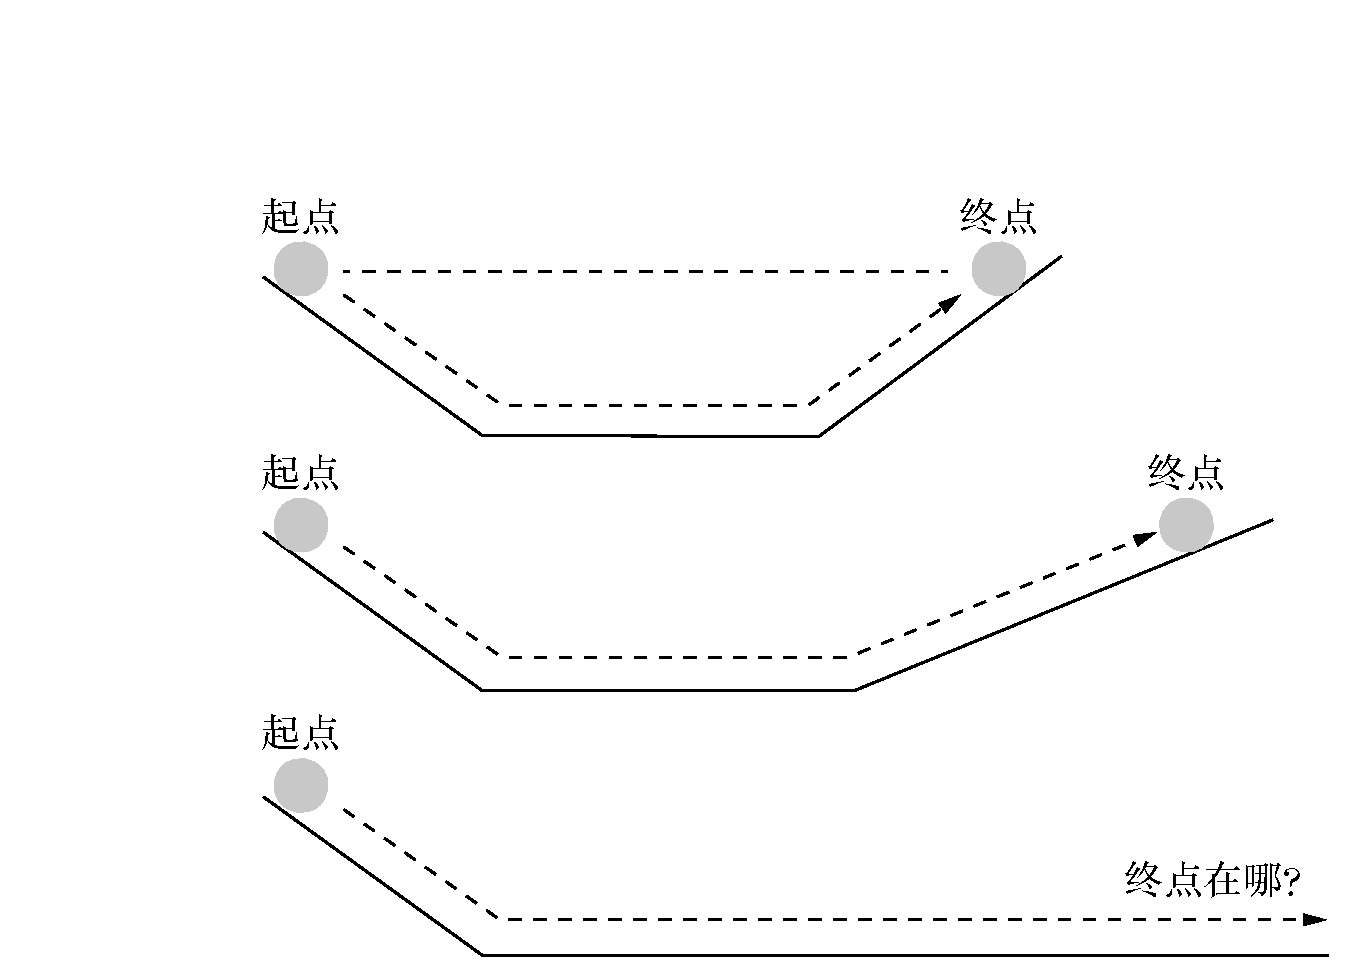
\includegraphics{Galileo}
    \caption{Galileo斜面实验}
    \labfig{Galileo_slope_experiment}
\end{marginfigure}

这个误差就是上面提到的单元内误差.这种误差在是心理学中的一种非常特殊的误差,在物理实验中就不存在这样误差,比如在Galileo的斜面实验(slope experiment),可以看到\reffig{Galileo_slope_experiment}中每个圆球都会上升到同一个高度,不同的球在各种属性上都是完全相同的,所以重复实验对物理属性匹配了的圆球就会有相同效果.但是对于人而言,每个人都不一样,都带着性别、性格、年龄、教育程度等进入实验室,而这些因素会影响行为,我们无法做到匹配完全相同的两个人.
这个变异在完全随机设计中给我们提供了一个随机误差的估计,所有的处理效应都是和它相比,尽管这部分变异不完全是随机的,不过对于完全随机设计而言已经没有更好的办法了.

从这个角度上来说,任何实验中每一组内都不可能只用一个被试,如果只有一个被试就没有变异了,起码两个人才有变异.

\subsection{评价}

完全随机实验设计的\textbf{优点}是,实验设计和实施简单,接受每个处理水平的被试数量可以不相等,不需要匹配被试,每个被试公接受一个处理水平.完全随机实验的统计分析和对结果的解释简单,并且与它的误差平方和相对应的自由度最大。因此,如果在不同的实验设计中得到的误差平方和相等,那么完全随机实验设计比其他实验设计更敏感.

完全随机实验设计的\textbf{缺点}是,它的组内变异并非全部由随机误差组成,其中还包括了被试的个体差异.虽然完全随机设计假设随机分配的各组被试在统计上是无差异的,但实际上被试的个体差异带来的无关变异是存在的,并且混杂在组内变异中,导致$F$比率的分母项加大, 从而使实验较为不敏感.另外,当实验中含多个处理水平时,需要的被试量也会较大.



\section{单因素随机区组实验设计}

\subsection{基本特点}
行为科学研究中,被试的个体差异是误差变异的重要来源.它常常会混淆实验处理效应,因此是无关变异.

方差分析用随机误差代表一些随机发生的因素带来的影响,如果某个效应带来的变异显著大于随因素带来的变异,我们认为这个效应不同于随机因素,是个在统计上有显著意义的效应.然而,在完全随机实验设计中,这个误差的衡量方式是所有被试间的个体差异,但是被试间的个体误差不能完全代表随机误差,因变量对其中某些因素是敏感的.在这些个体差异带来的无关变异中,随机区组设计找出影响因变量最大的,分离这个无关变量带来的变异,使误差效应变小,使这部分无关变异既不出现在处理效应中混淆处理作用的大小,也不出现在误差中降低检验力.这样在$F$检验中:
\[F=\frac{MSA}{MS_{\text{组内}}}\]

将$MSE$中由无关变量$B$带来的无关变异减去,得到
\[MSE=MS_{组内}-MSB\]

使误差效应更小,$F$更容易显著.

单因素随机区组设计适用于这样的情境:研究中有一个自变量,自变量有两个或多个水平$\left( P \geq 2 \right)$,研究中还有一个无关变量,也有两个或多个水平$\left( n \geq 2 \right)$,并且自变量的水平与无关变量的水平之间没有交互作用.

当无关变量是\textbf{被试变量}时, 一般首先将被试在这个无关变量上进行匹配,然后将他们随机分配给不同的实验处理.这样,区组内的被试在此无关变量上更加同质,他们接爱不同的处理水平时,可看作不受无关变量的影响,主要受处理的影响而区组之间的变异反映了无关变量的影响,我们可以利用方差分析技术区分出这一部分变异,经减少误差变异,获得对应效应的更精确估价.

另外环境因素也是潜在可考虑的区组变量,例职,每天的时间、每年的季节、地点、仪器等方面的因素也可以进行区组,经减少误差变异,\textbf{时间}是一个特别有效的区组变量,因为它常常还会带来一些附加自变量,如身体的生理周期、疲劳等.



\begin{margintable}
	\centering
	\caption{单因素随机区组实验设计中被试的分配}
	\labtab{one_way_ANOVA_block_subject}
	{
			\begin{tabular}{ccccc}
			\toprule
			 & $a_1$ & $a_2$ & $a_3$ & $a_4$ \\
			\midrule
			区组1 & $S_1$ & $S_2$ & $S_3$ & $S_4$ \\
			区组2 & $S_5$ & $S_6$ & $S_7$ & $S_8$ \\
			区组3 & $S_9$ & $S_{10}$ & $S_{11}$ & $S_{12}$ \\
			区组4 & $S_{13}$ & $S_{14}$ & $S_{15}$ & $S_{16}$ \\
			\bottomrule
		\end{tabular}	
	}
\end{margintable}

单因素随机区组实验设计中被试与处理的分配如\vreftab{one_way_ANOVA_block_subject},图中可以看出实验中有一个自变量,该自变量有4个水平.实验中还有一个无关变量,将16个被试在无关变量上进行匹配,分为4个区组,每个区组内4个同质被试,随机分配每个被试接受一个处理水平.

单因素随机区组的下标字母与单因素完全随机差不多,不同的是,完全随机设计中,每个处理内被试有多个,故$i$表示的是处理内第$i$个被试,每个处理都有$n$个被试;而在随机区组设计中,不存在这种处理内的被试,我们看到\vreftab{one_way_ANOVA_block_subject}中$a_1$下的4个被试又属于不同的区组.因此,现在的处理内的被试换成了区组,故一共有$n$个区组,$i$表示第$i$个区组.

\subsubsection{单因素随机区组实验设计模型}

\begin{definition}[单因素随机区组设计模型]
\labdef{one_way_ANOVA_block_model}
\begin{align*}
    Y_{ij} = \mu + \alpha _j +  & \pi _i + \varepsilon _{i\left(j\right)}\\
                                & \left( j=1,2,\cdots , p;i = 1,2,\cdots,n \right)
\end{align*}
其中

\begin{tabular}{lcl}
    $Y_{ij}$ & - & 被试在区组$i$和处理水平$j$上的分数 \\
    $\mu$ & - & 总体平均数 \\
    $\alpha _j$ & - & 水平$j$的处理效应 \\
    $\pi _i ^2$ & - & 区组效应,且$\pi _i ^2\sim N\left(0,\sigma _\pi ^2\right)$\\
    $\varepsilon_{i \left( j \right)}$ & - & 误差效应 \\
\end{tabular}
\end{definition}


%
%
%
%
\subsubsection{单因素随机区组实验设计检验的假说}



1.处理水平的总体平均数相等
\[ \mu _{.1} = \mu _{.2} = \cdots = \mu _{.p} \]

或处理效应等于0,即
\[ \alpha _j = 0 \]

2.区组的总体平均数相等
\[ \mu _{1.} = \mu _{2.} = \cdots = \mu _{n.} \]

或区组效应等于0,即
\[ H_0 : \pi _i ^2 = 0\]

因随机区组设计中假设区组变量和自变量间没有交互作用,所以在假设中就没有关于交互作用假设.

\subsection{实验设计和计算举例}
\subsubsection{研究问题}
我们仍利用第一节中文章的生字密度对阅读理解影响的研究做例子,由于考虑到学生的智力可能对阅读理解测验分数产生影响,但它又不是该实验中感兴趣的因素,我决定把学生的智力作为一个无关变量,通过实验设计将它的效应分离出去,以更好地探讨生字密度对阅读理解的影响.我选用了单因素随机区组实验设计.这时,我的研究假说、实验的自变量、因变量都是不变的,只是增加了一个无关变量.在实验实施前,我首选要给32个学生做智力测验,并按智力将学生分为8个区组,然后随机分配每个区组内的4个同质被试分别阅读一种生字密度的文章.

\subsubsection{数据计算}

\textbf{1.计算表}
%----------------------------单因素随机区组设计计算表
\begin{margintable}
	\centering
	\caption{单因素随机区组实验的$AS$表}
	\labtab{one_way_ANOVA_AS_TAB}
	{
		\begin{tabular}{ccccc|c}
			\toprule
    			 & $a_1$ &  $a_2$ &  $a_3$ &  $a_4$ & $\sum$ \\
    			     \midrule
                        区组1 & \cellcolor[rgb]{ .949,  .949,  .949}3 & \cellcolor[rgb]{ .949,  .949,  .949}4 & \cellcolor[rgb]{ .949,  .949,  .949}8 & \cellcolor[rgb]{ .949,  .949,  .949}9 & \cellcolor[rgb]{ .988,  .894,  .839}24 \\
                        区组2 & \cellcolor[rgb]{ .949,  .949,  .949}6 & \cellcolor[rgb]{ .949,  .949,  .949}6 & \cellcolor[rgb]{ .949,  .949,  .949}9 & \cellcolor[rgb]{ .949,  .949,  .949}8 & \cellcolor[rgb]{ .988,  .894,  .839}29 \\
                        区组3 & \cellcolor[rgb]{ .949,  .949,  .949}4 & \cellcolor[rgb]{ .949,  .949,  .949}4 & \cellcolor[rgb]{ .949,  .949,  .949}8 & \cellcolor[rgb]{ .949,  .949,  .949}8 & \cellcolor[rgb]{ .988,  .894,  .839}24 \\
                        区组4 & \cellcolor[rgb]{ .949,  .949,  .949}3 & \cellcolor[rgb]{ .949,  .949,  .949}2 & \cellcolor[rgb]{ .949,  .949,  .949}7 & \cellcolor[rgb]{ .949,  .949,  .949}7 & \cellcolor[rgb]{ .988,  .894,  .839}19 \\
                        区组5 & \cellcolor[rgb]{ .949,  .949,  .949}5 & \cellcolor[rgb]{ .949,  .949,  .949}4 & \cellcolor[rgb]{ .949,  .949,  .949}5 & \cellcolor[rgb]{ .949,  .949,  .949}12 & \cellcolor[rgb]{ .988,  .894,  .839}26 \\
                        区组6 & \cellcolor[rgb]{ .949,  .949,  .949}7 & \cellcolor[rgb]{ .949,  .949,  .949}5 & \cellcolor[rgb]{ .949,  .949,  .949}6 & \cellcolor[rgb]{ .949,  .949,  .949}13 & \cellcolor[rgb]{ .988,  .894,  .839}31 \\
                        区组7 & \cellcolor[rgb]{ .949,  .949,  .949}5 & \cellcolor[rgb]{ .949,  .949,  .949}3 & \cellcolor[rgb]{ .949,  .949,  .949}7 & \cellcolor[rgb]{ .949,  .949,  .949}12 & \cellcolor[rgb]{ .988,  .894,  .839}27 \\
                        区组8 & \cellcolor[rgb]{ .949,  .949,  .949}2 & \cellcolor[rgb]{ .949,  .949,  .949}3 & \cellcolor[rgb]{ .949,  .949,  .949}6 & \cellcolor[rgb]{ .949,  .949,  .949}11 & \cellcolor[rgb]{ .988,  .894,  .839}22 \\
                        \midrule
                              $\sum$ & \cellcolor[rgb]{ .886,  .937,  .855}35 & \cellcolor[rgb]{ .886,  .937,  .855}31 & \cellcolor[rgb]{ .886,  .937,  .855}56 & \cellcolor[rgb]{ .886,  .937,  .855}80 & \cellcolor[rgb]{ .867,  .922,  .969}202 \\

			\bottomrule
		\end{tabular}
	}
\end{margintable}
%----------------------------------------------------------------------------
\textbf{2.各种基本量的计算}
    \begin{align*}
        %----------------------------------------------------------
        %[Y]
            \frac{
                \left(
        	\sum\limits_{i=1}^{n} \sum\limits_{j=1}^{p}Y_{ij}
                \right)^2}
            {np}=& \colorbox[rgb]{ .867,  .922,  .969}{$[Y]$} = 
            \frac{
                \left(
        	    202
                \right)^2}
                {
                    \left(
        	           8
                    \right)^2
                    \left(
                        4
                    \right)^2
                }&=1275.125\\
        %----------------------------------------------------------
        %[AS]
            \sum\limits_{i=1}^{n} \sum\limits_{j=1}^{p}Y_{ij}^2=
            & \colorbox[rgb]{ .949,  .949,  .949}{$[AS]$} = 
            \left(
            	3
            \right)^2 +
            \left(
            	6
            \right)^2    +\cdots &=1544.000\\
        %----------------------------------------------------------
        %[A]    
            \sum\limits_{i=1}^{n}
            \frac
                {\left(
	            \sum\limits_{j=1}^{p}Y_{ij}
                \right)^2}
                {n}=
            &\colorbox[rgb]{ .886,  .937,  .855}{$[A]$}=
            \frac{\left(35\right)^2}{8}+\frac{\left(31\right)^2}{8}+\cdots&=1465.250\\
        %---------------------------------------------------------
        %[S]
            \sum\limits_{i=1}^{n}
            \frac
            {
                \sum\limits_{j=1}^{p}\left(Y_{ij} \right)^2
            }
            {
                p            
            }            
            =&\colorbox[rgb]{ .988,  .894,  .839}{$[S]$}
            =\frac{\left( 24 \right)^2}{4} + \frac{\left( 29 \right)^2}{4} + \cdots &= 1301.000
    \end{align*}
%---------------------------------------------
\textbf{3.平方和的分解}

\begin{definition}[单因素随机区组设计平方和的分解]
\labdef{one_way_ANOVA_block_variance_breakthrough}
\begin{alignat*}{2}
   & SS_{\text{总变异}} &&= SS_{\text{处理间}} + SS_{\text{处理内}}\\
   &                    &&= SSA + (SS_{\text{区组}} + SS_{\text{残差}})
\end{alignat*}
\end{definition}
\begin{alignat*}{3}
    &    SS_{\text{总变异}} &&     =[AS]-[Y]                                 && =268.875\\
    &    SSA                &&    =[A]-[Y]                                  && =190.125\\
    &    SS_{\text{区组}}   &&    =[S]-[Y]                                   && =25.750\\
    &    SS_{\text{残差}}   &&    =SS_{\text{总变异}}-SSA-SS_{\text{区组}}    &&=52.875
\end{alignat*}
%----------------------
\textbf{4.方差分析表及结果解释}
\begin{table}[h]
	\centering
	\caption{单因素随机区组实验的方差分析表}
	\labtab{one_way_block_ANOVA_Tab}
	{
		\begin{tabular}{lrrcrrr}
			\toprule
			\multicolumn{1}{c}{变异源} & \multicolumn{1}{c}{$SS$} & \multicolumn{1}{c}{$df$} & \multicolumn{1}{c}{$MS$} & \multicolumn{1}{c}{$F$} & \multicolumn{1}{c}{$p$} \\
			\midrule
			$A$(生字密度) & 190.125 & $p-1=3$ & 63.375 & 25.170 & $<$ .001  \\
			区组(智力) & 25.850 & $n-1=7$ & 3.696 & 1.47 & 0.23   \\
			残差 & 52.875 & $(n-1)(p-1)=21$ & 2.518\\
			\midrule
			总计 & 268.875 & $np-1=31$ & & &\\
			\bottomrule
			% \addlinespace[1ex]
			% \multicolumn{6}{p{0.5\linewidth}}{\textit{Note.} Type III Sum of Squares} \\
		\end{tabular}
	}
\end{table}

方差分析可以看出,实验中的自变量——生字密度的效应是统计显著的$\left( F(3,21)=25.170, p < .001 \right)$,说明学生对生字密度不同的文章的阅读理解有显著差别.实验中无关变量——智力的效应是统计上不显著的$\left( F \left( 7,21 \right) = 1.47, p > .05 \right)$,表明本实验中智力不同的学生的阅读理解 没有明显差异.方差分析表中还可以看出,生字密度和智力的$F$检验都使用了同一个误差项$MSE=2.518$.

\textbf{5.平方和与自由度分解图}


\subsection{一些解释}
\textbf{1.各种平方和的意义}

\begin{description}
\item[$SS_{\text{总变异}}$]——在随机区组实验中,总平方和应首先分解为处理间平方和处理内平方和应首先分解 为处理间平方和处理内平方和.
\item[$SS_{\text{处理间}}$]——处理间平方和指所有由实验处理引起的变异,在单因素设计中指$A$因素的处理效应$SSA$
\item[$SS_{\text{处理内}}$]——在随机区组实验中,处理内平方和可进一步分解为两部分:区组平方和和误差平方和.
\item[$SS_{\text{区组}}$]——区组效应,在该实验中指总变异中由被试的智力引起的变异.
\item[$SS_{\text{残差}}$]——残差指总变异中不能被实验处理和区组效应解释的变异.在随机区组实验设计中,接受同实验条件的同质被试只有一个,因此,不能计算单元内误差,而残差作为误差变异的估计.残差的计算是从总变异中减去处理效应和区组变异.
\end{description}

\textbf{2.做区组的方法}

除了感兴趣的自变量外,还有很多无关就量都影响因变量.如果发现一个变量特别影响因变量,但对其效应不感兴趣,可以考虑将其作一个区组.本例中区组变量是智力,我们知道一个孩子的智力情况会影响他的阅读理解,如果一个组里都是智力低的孩子,一个组里都是智力高的孩子.若智力高的组分配的是低生字密度,生字密度和智力都会促进阅读理解,处理效应被加大,当本身处理效应不显著时,会面临错误判定处理效应显著的失误;若智力高的组分配的是高生字密度,自变量效应方向和无关变量方向相反,它们抵消后会使处理效应被掩盖,造成处理效应不显著.

\textbf{3.随机区组提高实验敏感性的体现}

前面我提到从$F$值的大小思考实验的敏感性,单因素完全随机的$F$值:
\[ F=\frac{MSA}{MS_{\text{组内}}} \]

单因素随机区组设计将$SS_{组内}$进一步分解为$SS_{\text{区组}}$和$SS_{\text{残差}}$,既然区组变量带来的变异不是随机误差,因此将其从组内误差中分离出来,这样误差项就减小了,从而单因素随机区组的$F$值就是:
\[ F = \frac{MSA}{MS_{\text{残差}}} \]

而$MS_{\text{残差}} < MS_{\text{组内}}$,因而提升了实验的敏感性.从数据上,我们可以看到,在\vreftab{one_way_ANOVA_Tab}中,组内误差是78.750,在同样的数据用了随机区组的算法后,\vreftab{one_way_block_ANOVA_Tab}中可以看出,将组内误差分解成了区组带来的无关变异25.850,和剩余的残差52.875.完全随机的$F$是22.533,在随机区组中$F$是25.170,这看上去没有提升多少,原因是这组数据中区组变量的效应是不显著的,可以看到残差项还是很大,说明这个随机区组变量并不是特别有效.

那么什么是有效的随机区组设计呢?
在\vreftab{one_way_ANOVA_AS_TAB}中右边红色的数据是对把自变量处理水平$a_1,a_2,a_3,a_4$合并起来的数据,这样这个数据只和集中趋势和区组无关变量带来的变异相关,我们把它按小到大排个序:
\[ 19,22,24,24,26,27,29,21 \]

这和绿色的数据:
\[ 31,35,56,80 \]

相比,变异就小了很多.一个好的区组设计应该让红色的那部分数据呈现一个明显的梯度,让它们之间相差得大一点,这样就可以带走更多变异.这点不是实验操作上可以保证的,主要是要看这个区组变量是不是一个有效的区组变量,是否对因变量有较大影响.

\textbf{4.残差的实质}

从方差分析中的自由度(见\vreftab{one_way_block_ANOVA_Tab})知,残差的自由度是$(p-1)(n-1)$,这个形式表明这个残差本质是个交互作用.现在还不是时候从根本上揭示残差的实质.

随机区组中,用残差来估价随机误差,今后我们将看到,所有的误差项只有两种形式,一种是单元内误差(当有同质被试接受相同的处理时产生),一种是残差(实验是交互作用).在随机区组设计中,由于没有接受相同处理的同质被试,故不存在单元内误差.

\subsection{评价}
随机区组的\textbf{优点}是,在许多研究情境中,它比完全随机实验设计更加有效.这是由于它使研究者从总变异中分离出了一个无关变量的效应,从而减小了实验误差,可获得对处理效应的更加精确的估价.随机区组实验设计可使用于含任何处理水平数的实验中,并且区组的数量也不受限制,因而有较好的灵活性.

随机区组实验设计的\textbf{缺点}是,如实验中含有多处理水平,可能给形成同质区组、寻找同质被试带来困难.另外,使用随机区组设计比使用完全随机设计有更多的限定,例如使用随机区组实验设计的前提假设是,实验中的自变量与无关变量之间没有交互作用.如果交互作用是存在的,使用随机区组实验设计是不合适的.这在一定程度上限制了随机区组实验设计的应用.但由于无法对该残差的显著性进行检验,故对于这个误差的估计是否合理就没有检验的方法.

\subsection{经典随机区组设计的改进}
\subsubsection{基本思想}
经典随机区组设计中,误差用残差衡量,它的实质是区组变量与自变量间的交互作用,问题是我们无法保证它们间一定不存在交互作用,我们甚至没有检验这个交互作用显著性的手段.

单元内误差是一定是一个可靠的误差估计,不过在经典随机区组设计中没有接受相同处理的同质被试,那对其进行改进即可,让区组内人数扩大,使接受同一个处理和在同一个区组内的被试有多个,这样可以算出单元内误差,检验残差是否显著.

\subsubsection{评价}
我们力求区组内被试同质,但是实际上很难做到.本例来说,区组变量是智力,这是一个连续变量.增加区组内被试时,有很大可有使区组内的变异变大,很有可能让区组间的变小.

所以随机区组设计不会用这种方式.

\section{单因素拉丁方实验设计}

拉丁方设计最大特色是同时计算了残差和单元内误差,扩展了区组实验设计.对于完全随机方差分析中的$F$检验而言:
\[ F=\frac{MSA}{MS_{\text{组内}}} \qquad MS_{\text{组内}}=\text{无关变异}+\text{随机误差} \]

由于完全随机设计中误差项$MSE$中混入了个体差异和一些其它的无关变异,所以随机区组设计找到一个影响较大的无关变异,计算其大小并从$MSE$中分离,这样新的$MSE$就等于$MSE_{\text{组内}}-MS_{\text{区组}}$,误差项减小,可以提高实验的精度.
不过这样还不够,首先,对于影响因变量的无关变量不止有一个,也许除了生字密度学、生的智力外,还有别的无关变量对阅读理解有较大影响.故我们希望可以再分离出一个无关变量的效应;
其次,随机区组的误差是否是一个合理的误差也不清楚
所以我还希望在每一个区组内加入多个被试,以检验残差的是否显著.

总的来说,拉丁方实验设计同时分离两个无关变量的效应,同时通过分配多个被试给同一自变量水平和无关变量水平的结合,使得可以计算出单元内误差来检验残差是否显著.不过该设计对两个无关变量有较大要求.拉丁方实验设计适合下列条件:

\begin{description}
\item[1.自变量和无关变量的水平限制] 自变量的水平和两个无关变量的水平相等,即自变量水平是$p$ $(p\geq 2)$,两个无关变量水平都是$p$ $(p\geq 2)$;
\item[2.自变量与无关变量无交互作用] 如果这个假设不能满足峄实验中的一个或多个效应的检验可能有偏差
\item[3.拉丁方限制]随机分配处理立平给$p^2$个方格单元,每个处理水平仅在每行、每列中出现一次
\end{description}

%-----------begin连续的拉丁方快
\begin{margintable}
  \caption{$2\times 2$拉丁方快}
  \labtab{lantin_square_2_2}
    \begin{tabular}{cc}
    A     & B \\
    B     & A \\
    \end{tabular}
\end{margintable}

\begin{margintable}
  \caption{$3\times 3$拉丁方快}
  \labtab{lantin_square_3_3}
    \begin{tabular}{ccc}
    A  &  B  &  C\\
    B  &  C  &  A\\
    C  &  A  &  B\\
    \end{tabular}
\end{margintable}

\begin{margintable}
  \caption{$4\times 4$拉丁方快}
  \labtab{lantin_square_4_4}
    \begin{tabular}{cccc}
    A     & B     & C     & D \\
    B     & C     & D     & A \\
    C     & D     & A     & B \\
    D     & A     & B     & C \\
    \end{tabular}
\end{margintable}

\begin{margintable}
  \caption{$5\times 5$拉丁方快}
  \labtab{lantin_square_5_5}
    \begin{tabular}{ccccc}
    A     & B     & C     & D     & E \\
    B     & C     & D     & E     & A \\
    C     & D     & E     & A     & B \\
    D     & E     & A     & B     & C \\
    E     & A     & B     & C     & D \\
    \end{tabular}
\end{margintable}
%---------------------end连续的拉丁方快

我列出了五个拉丁方格:\vreftab{lantin_square_2_2},\vreftab{lantin_square_3_3},\vreftab{lantin_square_4_4},\vreftab{lantin_square_5_5},从列子中可以看到拉丁方格每一行每一列每一个字母只出现一次,下面以$4\times 4$拉丁方表格介绍一下拉丁方格随机化的方法:

\begin{table}[h]
  \caption{拉丁方格标准化方块的随机化}
  \labtab{lantin_square_norm}
    \begin{tabular}{ccccccccccc}
          & \multicolumn{4}{c}{标准块}       &       &       & \multicolumn{4}{c}{随机化行} \\
          & 1     & 2     & 3     & 4     &       &       & 1     & 2     & 3     & 4 \\
    1     & \cellcolor[rgb]{ .851,  .882,  .949}A & \cellcolor[rgb]{ .851,  .882,  .949}B & \cellcolor[rgb]{ .851,  .882,  .949}C & \cellcolor[rgb]{ .851,  .882,  .949}D &       & 3     & \cellcolor[rgb]{ .886,  .937,  .855}C & \cellcolor[rgb]{ .886,  .937,  .855}D & \cellcolor[rgb]{ .886,  .937,  .855}A & \cellcolor[rgb]{ .886,  .937,  .855}B \\
    2     & \cellcolor[rgb]{ 1,  .949,  .8}B & \cellcolor[rgb]{ 1,  .949,  .8}C & \cellcolor[rgb]{ 1,  .949,  .8}D & \cellcolor[rgb]{ 1,  .949,  .8}A &       & 1     & \cellcolor[rgb]{ .851,  .882,  .949}A & \cellcolor[rgb]{ .851,  .882,  .949}B & \cellcolor[rgb]{ .851,  .882,  .949}C & \cellcolor[rgb]{ .851,  .882,  .949}D \\
    3     & \cellcolor[rgb]{ .886,  .937,  .855}C & \cellcolor[rgb]{ .886,  .937,  .855}D & \cellcolor[rgb]{ .886,  .937,  .855}A & \cellcolor[rgb]{ .886,  .937,  .855}B &       & 2     & \cellcolor[rgb]{ 1,  .949,  .8}B & \cellcolor[rgb]{ 1,  .949,  .8}C & \cellcolor[rgb]{ 1,  .949,  .8}D & \cellcolor[rgb]{ 1,  .949,  .8}A \\
    4     & \cellcolor[rgb]{ .929,  .929,  .929}D & \cellcolor[rgb]{ .929,  .929,  .929}A & \cellcolor[rgb]{ .929,  .929,  .929}B & \cellcolor[rgb]{ .929,  .929,  .929}C &       & 4     & \cellcolor[rgb]{ .929,  .929,  .929}D & \cellcolor[rgb]{ .929,  .929,  .929}A & \cellcolor[rgb]{ .929,  .929,  .929}B & \cellcolor[rgb]{ .929,  .929,  .929}C \\
          &       &       &       &       &       &       &       &       &       &  \\
          & \multicolumn{4}{c}{随机化行}      &       &       & \multicolumn{4}{c}{随机化列} \\
          & 1     & 2     & 3     & 4     &       &       & 4     & 3     & 1     & 2 \\
    3     & \cellcolor[rgb]{ .851,  .882,  .949}C & \cellcolor[rgb]{ .988,  .894,  .839}D & \cellcolor[rgb]{ .929,  .929,  .929}A & \cellcolor[rgb]{ .886,  .937,  .855}B &       & 3     & \cellcolor[rgb]{ .886,  .937,  .855}B & \cellcolor[rgb]{ .929,  .929,  .929}A & \cellcolor[rgb]{ .851,  .882,  .949}C & \cellcolor[rgb]{ .988,  .894,  .839}D \\
    1     & \cellcolor[rgb]{ .851,  .882,  .949}A & \cellcolor[rgb]{ .988,  .894,  .839}B & \cellcolor[rgb]{ .929,  .929,  .929}C & \cellcolor[rgb]{ .886,  .937,  .855}D &       & 1     & \cellcolor[rgb]{ .886,  .937,  .855}D & \cellcolor[rgb]{ .929,  .929,  .929}C & \cellcolor[rgb]{ .851,  .882,  .949}A & \cellcolor[rgb]{ .988,  .894,  .839}B \\
    2     & \cellcolor[rgb]{ .851,  .882,  .949}B & \cellcolor[rgb]{ .988,  .894,  .839}C & \cellcolor[rgb]{ .929,  .929,  .929}D & \cellcolor[rgb]{ .886,  .937,  .855}A &       & 2     & \cellcolor[rgb]{ .886,  .937,  .855}A & \cellcolor[rgb]{ .929,  .929,  .929}D & \cellcolor[rgb]{ .851,  .882,  .949}B & \cellcolor[rgb]{ .988,  .894,  .839}C \\
    4     & \cellcolor[rgb]{ .851,  .882,  .949}D & \cellcolor[rgb]{ .988,  .894,  .839}A & \cellcolor[rgb]{ .929,  .929,  .929}B & \cellcolor[rgb]{ .886,  .937,  .855}C &       & 4     & \cellcolor[rgb]{ .886,  .937,  .855}C & \cellcolor[rgb]{ .929,  .929,  .929}B & \cellcolor[rgb]{ .851,  .882,  .949}D & \cellcolor[rgb]{ .988,  .894,  .839}A \\
    \end{tabular}%
\end{table}

单因素拉丁方实验设计被试分配到处理上的例子如\vreftab{latin_subject_treatment}.从表中可以看出,实验中的自变量$A$有4个水平,无关变量$B$和无关变量$C$也各有4个水平,形成$4\times 4$的拉丁方格,32个被试参加了实验,每个方格内有2个被试,每个被试只接受一种独特的实验条件处理.

\begin{margintable}
  \centering
  \caption{单因素拉丁方实验设计中被试的分配}
    \begin{tabular}{ccccc}
          & $c_1$ & $c_2$ & $c_3$ & $c_4$ \\
    \multirow{3}[0]{*}{$b_1$} & \cellcolor[rgb]{ .851,  .882,  .949}$a_1$ & \cellcolor[rgb]{ .851,  .882,  .949}$a_2$ & \cellcolor[rgb]{ .851,  .882,  .949}$a_3$ & \cellcolor[rgb]{ .851,  .882,  .949}$a_4$ \\
          & \cellcolor[rgb]{ .886,  .937,  .855}$S_1$ & \cellcolor[rgb]{ .886,  .937,  .855}$S_9$ & \cellcolor[rgb]{ .886,  .937,  .855}$S_{17}$ & \cellcolor[rgb]{ .886,  .937,  .855}$S_{25}$ \\
          & \cellcolor[rgb]{ .886,  .937,  .855}$S_2$ & \cellcolor[rgb]{ .886,  .937,  .855}$S_{10}$ & \cellcolor[rgb]{ .886,  .937,  .855}$S_{18}$ & \cellcolor[rgb]{ .886,  .937,  .855}$S_{26}$ \\
    \multirow{3}[0]{*}{$b_2$} & \cellcolor[rgb]{ .851,  .882,  .949}$a_2$ & \cellcolor[rgb]{ .851,  .882,  .949}$a_3$ & \cellcolor[rgb]{ .851,  .882,  .949}$a_4$ & \cellcolor[rgb]{ .851,  .882,  .949}$a_1$ \\
          & \cellcolor[rgb]{ .886,  .937,  .855}$S_3$ & \cellcolor[rgb]{ .886,  .937,  .855}$S_{11}$ & \cellcolor[rgb]{ .886,  .937,  .855}$S_{19}$ & \cellcolor[rgb]{ .886,  .937,  .855}$S_{27}$ \\
          & \cellcolor[rgb]{ .886,  .937,  .855}$S_4$ & \cellcolor[rgb]{ .886,  .937,  .855}$S_{12}$ & \cellcolor[rgb]{ .886,  .937,  .855}$S_{20}$ & \cellcolor[rgb]{ .886,  .937,  .855}$S_{28}$ \\
    \multirow{3}[0]{*}{$b_3$} & \cellcolor[rgb]{ .851,  .882,  .949}$a_3$ & \cellcolor[rgb]{ .851,  .882,  .949}$a_4$ & \cellcolor[rgb]{ .851,  .882,  .949}$a_1$ & \cellcolor[rgb]{ .851,  .882,  .949}$a_2$ \\
          & \cellcolor[rgb]{ .886,  .937,  .855}$S_5$ & \cellcolor[rgb]{ .886,  .937,  .855}$S_{13}$ & \cellcolor[rgb]{ .886,  .937,  .855}$S_{21}$ & \cellcolor[rgb]{ .886,  .937,  .855}$S_{29}$ \\
          & \cellcolor[rgb]{ .886,  .937,  .855}$S_6$ & \cellcolor[rgb]{ .886,  .937,  .855}$S_{14}$ & \cellcolor[rgb]{ .886,  .937,  .855}$S_{22}$ & \cellcolor[rgb]{ .886,  .937,  .855}$S_{30}$ \\
    \multirow{3}[0]{*}{$b_4$} & \cellcolor[rgb]{ .851,  .882,  .949}$a_4$ & \cellcolor[rgb]{ .851,  .882,  .949}$a_1$ & \cellcolor[rgb]{ .851,  .882,  .949}$a_2$ & \cellcolor[rgb]{ .851,  .882,  .949}$a_3$ \\
          & \cellcolor[rgb]{ .886,  .937,  .855}$S_7$ & \cellcolor[rgb]{ .886,  .937,  .855}$S_{15}$ & \cellcolor[rgb]{ .886,  .937,  .855}$S_{23}$ & \cellcolor[rgb]{ .886,  .937,  .855}$S_{31}$ \\
          & \cellcolor[rgb]{ .886,  .937,  .855}$S_8$ & \cellcolor[rgb]{ .886,  .937,  .855}$S_{16}$ & \cellcolor[rgb]{ .886,  .937,  .855}$S_{24}$ & \cellcolor[rgb]{ .886,  .937,  .855}$S_{32}$ \\
    \end{tabular}%
  \labtab{latin_subject_treatment}
\end{margintable}

\begin{definition}[单因素拉丁方设计模型]
\labdef{one_way_latin_model}
\begin{align*}
    Y_{ijkl} = \mu + \alpha _j + \beta _k & + \gamma _l + \varepsilon _{pooled}\\
                                          &(j=1,2,\cdots,p;i=1,2,\cdots,n)\\
                                          &(k=1,2,\cdots,p;l=1,2,\cdots,p)
\end{align*}

其中

\begin{tabular}{ccl}
    $Y_{ijkl}$     & - &    两无关变量在第$j,k$个水平上,被试$i$的分数\\ 
    $\mu$          & - &    总体平均值或真值\\
    $\alpha _j$    & - &    自变量水平$j$的处理效应\\
    $\beta _k$     & - &    无关变量$B$水平$k$的变异\\
    $\gamma _l$    & - &    无关变量$C$水平$l$的变异\\
    $\varepsilon _{pooled}$ &-& 合并误差
\end{tabular}

\end{definition}

模型中的$\varepsilon _{pooled}$,pooled指的是“集合的,集中的”,这是两项误差的合并,这点我在后面会介绍.

拉丁方实验设计适合检验的假说是:

(1)处理水平的总体平均数相等,即:
\[ H_0 : \mu _{1..} = \mu _{2..} = \cdots = \mu _{p..}\]

或因素$A$效应等于0,即:
\[ H_0 : \alpha _j = 0 \]

(2)无关变量(横行)的总体平均数相等,即
\[ H_0 : \mu _{.1.} = \mu _{.2.} = \cdots = \mu _{.p.} \]

或无关变量$B$的效应等于0,即
\[ \beta _k = 0 \]

(3)无关变量(纵行)的总体平均数相等,即
\[ H_0 : \mu _{..1} = \mu _{..2} = \cdots = \mu _{..p} \]

或无关变量$C$的效应等于0,即
\[ \gamma _l = 0 \]




 \subsection{实验设计与计算举例}
 
 \subsubsection{研究的问题与实验设计}
 
 \subsubsection{实验数据及其计算}

\textbf{计算表}

%---ABCS表--------------------------------------------------------------
\begin{margintable}
  \centering
  \caption{拉丁方设计$ABCS$表}
    \begin{tabular}{ccccc}
    \toprule
          & $c_1$ & $c_2$ & $c_3$ & $c_4$ \\
    \midrule
          & $a_1$ & $a_2$ & $a_3$ & $a_4$ \\
    \multirow{2}[0]{*}{$b_1$} & \cellcolor[rgb]{ .949,  .949,  .949}3 & \cellcolor[rgb]{ .949,  .949,  .949}2 & \cellcolor[rgb]{ .949,  .949,  .949}6 & \cellcolor[rgb]{ .949,  .949,  .949}9 \\
          & \cellcolor[rgb]{ .949,  .949,  .949}4 & \cellcolor[rgb]{ .949,  .949,  .949}3 & \cellcolor[rgb]{ .949,  .949,  .949}5 & \cellcolor[rgb]{ .949,  .949,  .949}8 \\
          & $a_2$ & $a_3$ & $a_4$ & $a_1$ \\
    \multirow{2}[0]{*}{$b_2$} & \cellcolor[rgb]{ .949,  .949,  .949}8 & \cellcolor[rgb]{ .949,  .949,  .949}3 & \cellcolor[rgb]{ .949,  .949,  .949}4 & \cellcolor[rgb]{ .949,  .949,  .949}7 \\
          & \cellcolor[rgb]{ .949,  .949,  .949}7 & \cellcolor[rgb]{ .949,  .949,  .949}2 & \cellcolor[rgb]{ .949,  .949,  .949}3 & \cellcolor[rgb]{ .949,  .949,  .949}6 \\
          & $a_3$ & $a_4$ & $a_1$ & $a_2$ \\
    \multirow{2}[0]{*}{$b_3$} & \cellcolor[rgb]{ .949,  .949,  .949}8 & \cellcolor[rgb]{ .949,  .949,  .949}12 & \cellcolor[rgb]{ .949,  .949,  .949}5 & \cellcolor[rgb]{ .949,  .949,  .949}6 \\
          & \cellcolor[rgb]{ .949,  .949,  .949}9 & \cellcolor[rgb]{ .949,  .949,  .949}13 & \cellcolor[rgb]{ .949,  .949,  .949}6 & \cellcolor[rgb]{ .949,  .949,  .949}4 \\
          & $a_4$ & $a_1$ & $a_2$ & $a_3$ \\
    \multirow{2}[0]{*}{$b_4$} & \cellcolor[rgb]{ .949,  .949,  .949}5 & \cellcolor[rgb]{ .949,  .949,  .949}8 & \cellcolor[rgb]{ .949,  .949,  .949}12 & \cellcolor[rgb]{ .949,  .949,  .949}7 \\
          & \cellcolor[rgb]{ .949,  .949,  .949}4 & \cellcolor[rgb]{ .949,  .949,  .949}7 & \cellcolor[rgb]{ .949,  .949,  .949}11 & \cellcolor[rgb]{ .949,  .949,  .949}5 \\
        \bottomrule
    \end{tabular}
  \labtab{latin_square_ABCS_tab}
\end{margintable}

%-----------------------------------------------------------------

%---ABC表
\begin{margintable}
  \centering
  \caption{拉丁方设计$ABC$表}

    \begin{tabular}{ccccc|c}
    \toprule
          & $c_1$ & $c_2$ & $c_3$ & $c_4$ & $\sum$ \\
    \midrule
          & $n=2$ &       &       &       &  \\
          & $a_1$ & $a_2$ & $a_3$ & $a_4$ &  \\
    $b_1$ & \cellcolor[rgb]{ .886,  .937,  .855}7 & \cellcolor[rgb]{ .886,  .937,  .855}5 & \cellcolor[rgb]{ .886,  .937,  .855}11 & \cellcolor[rgb]{ .886,  .937,  .855}17 & \cellcolor[rgb]{ 1,  .949,  .8}40 \\
          & $a_2$ & $a_3$ & $a_4$ & $a_1$ &  \\
    $b_2$ & \cellcolor[rgb]{ .886,  .937,  .855}15 & \cellcolor[rgb]{ .886,  .937,  .855}5 & \cellcolor[rgb]{ .886,  .937,  .855}7 & \cellcolor[rgb]{ .886,  .937,  .855}13 & \cellcolor[rgb]{ 1,  .949,  .8}40 \\
          & $a_3$ & $a_4$ & $a_1$ & $a_2$ &  \\
    $b_3$ & \cellcolor[rgb]{ .886,  .937,  .855}17 & \cellcolor[rgb]{ .886,  .937,  .855}25 & \cellcolor[rgb]{ .886,  .937,  .855}11 & \cellcolor[rgb]{ .886,  .937,  .855}10 & \cellcolor[rgb]{ 1,  .949,  .8}63 \\
          & $a_4$ & $a_1$ & $a_2$ & $a_3$ &  \\
    $b_4$ & \cellcolor[rgb]{ .886,  .937,  .855}9 & \cellcolor[rgb]{ .886,  .937,  .855}15 & \cellcolor[rgb]{ .886,  .937,  .855}23 & \cellcolor[rgb]{ .886,  .937,  .855}12 & \cellcolor[rgb]{ 1,  .949,  .8}59 \\
    $\sum$ & \cellcolor[rgb]{ .839,  .863,  .894}48 & \cellcolor[rgb]{ .839,  .863,  .894}50 & \cellcolor[rgb]{ .839,  .863,  .894}52 & \cellcolor[rgb]{ .839,  .863,  .894}52 & \cellcolor[rgb]{ .867,  .922,  .969}202 \\
    \bottomrule
    \end{tabular}

  \labtab{latin_square_ABC_tab}
\end{margintable}


%---------A表
\begin{margintable}
  \centering
  \caption{拉丁方设计$A$表}
    \begin{tabular}{cccc}
    \toprule
    \multicolumn{1}{c}{$a_1$} & \multicolumn{1}{c}{$a_2$} & \multicolumn{1}{c}{$a_3$} & \multicolumn{1}{c}{$a_4$} \\
    \midrule
    \multicolumn{1}{l}{$np=8$} &       &       &  \\
    \rowcolor[rgb]{ .957,  .69,  .518} 35    & 31    & 56    & 80 \\
    \bottomrule
    \end{tabular}
  \labtab{latin_square_A_tab}
\end{margintable}

\textbf{2.各种基本量的计算}

\begin{align*}
    \sum\limits_{i=1}^{n}\sum\limits_{k=l}^{p}\sum\limits_{l=1}^{p}Y_{ijkl}&=3+4+\cdots=202.000\\
    \frac{\sum\limits_{l=1}^p{\sum\limits_{k=1}^p{\sum\limits_{i=1}^n{Y_{ijkl}}}}}{np^2}=\left[ Y \right] &=\frac{\left( 202 \right) ^2}{\left( 2 \right) \left( 4 \right) ^2}\\
    \sum\limits_{l=1}^p{\sum\limits_{k=1}^p{\sum\limits_{i=1}^n{\left( Y_{ijkl}^{2} \right)}}}&=\left[ ABCS \right] =\left( 3 \right) ^2+\left( 4 \right) ^2+\cdots =1544.000\\
    \sum\limits_{l=1}^p{\sum\limits_{k=1}^p{\frac{\left( \sum\limits_{i=1}^n{Y_{ijkl}} \right) ^2}{n}}}&=\left[ ABC \right] =\frac{\left( 7 \right) ^2}{2}+\frac{\left( 5 \right) ^2}{2}+\cdots =1533.000\\
     &=\left[ A \right] =\frac{\left( 35 \right) ^2}{8}+\frac{\left( 31 \right) ^2}{8}+\cdots =1465.250\\
    \sum\limits_{k=1}^p{\frac{\left( \sum\limits_{l=1}^p{\sum\limits_{i=1}^n{Y_{ijkl}}} \right) ^2}{np}}&=\left[ B \right] =\frac{\left( 40 \right) ^2}{8}+\frac{\left( 40 \right) ^2}{8}+\cdots =1331.250\\
    \sum\limits_{l=1}^p{\frac{\left( \sum\limits_{k=1}^p{\sum\limits_{i=1}^n{Y_{ijkl}}} \right) ^2}{np}}&=\left[ C \right] =\frac{\left( 48 \right) ^2}{8}+\frac{\left( 50 \right) ^2}{8}+\cdots =1276.500\\
\end{align*}


\texfbf{3.平方和分解与计算}
\begin{alignat*}{4}
   & SS_{\text{总变异}} & &= SS_{\text{处理间}} & & +SS_{\text{处理内}}\\
   &                    & &= SSA               & & +\left( SSB + SSC + SS_{\text{单元内}} + SS_{\text{残差}}  \right)
\end{alignat*}


\begin{alignat*}{3}
    & SS_{\text{总变异}} && =[ABCS]-[Y] && =268.875\\
    & SSA               &&  =[A]   - [Y] && =190.125\\
    &SSB               && =[B] -[Y]&&=56.125\\
    & SSC              && =[C]-[Y] &&= 1.375\\
    & SS_{\text{残差}} && = {[ABC]-[Y]}-SSA-SSB-SSC && =10.250\\
    & SS_{\text{单元内}} && = SS_{\text{总变异}}-SSA-SSB-SSC-SS_{\text{残差}} && = 11.000
\end{alignat*}


\textbf{4.方差分析表及对结果的解释}

\begin{table}[h]
	\centering
	\caption{单因素拉丁方实验的方差分析表}
	\labtab{one_way_latin_ANOVA_Tab}
	{
		\begin{tabular}{lrrcrrr}
			\toprule
			\multicolumn{1}{c}{变异源} & \multicolumn{1}{c}{$SS$} & \multicolumn{1}{c}{$df$} & \multicolumn{1}{c}{$MS$} & \multicolumn{1}{c}{$F$} & \multicolumn{1}{c}{$p$} \\
			\midrule
			A(生字密度) & 190.125 & $p-1=3$ & 63.375 & 25.170 & $<$.001  \\
			B(班级) & 56.125 & $p-1=3$ & 18.708 & 27.19 & $<$.001   \\
			C(实验时间) & 1.375 & $p-1=3$ & 0.458 & 0.67 &  0.58  \\
			残差 & 52.875 & $(p-1)(p-2)=6$ & 1.708 & 2.48 & 0.18\\
			单元内误差 & 11.000 & $p^2(n-1)=16$ & 0.688\\
			\midrule
			总计 & 268.875 & $np^2-1=31$ & & &\\
			\bottomrule
			% \addlinespace[1ex]
			% \multicolumn{6}{p{0.5\linewidth}}{\textit{Note.} Type III Sum of Squares} \\
		\end{tabular}
	}
\end{table}

\textbf{5.平方和与自由度的分解}

\subsection{一些解释}

\subsection{评价}

\section{单因素被试内实验设计}

拉丁方实验设计模型
\[ Y_{ij} = \mu + \alpha _j + \pi _i + \varepsilon _{ij} \]

%----------------------------单因素被试内设计计算表
\begin{margintable}
	\centering
	\caption{单因素被试内设计的$AS$表}
	\labtab{one_way_repeated_ANOVA_AS_TAB}
	{
		\begin{tabular}{cccccc}
			\toprule
    			 & $a_1$ &  $a_2$ &  $a_3$ &  $a_4$ & $\sum$ \\
    			     \midrule
                        被试1 & \cellcolor[rgb]{ .949,  .949,  .949}3 & \cellcolor[rgb]{ .949,  .949,  .949}4 & \cellcolor[rgb]{ .949,  .949,  .949}8 & \cellcolor[rgb]{ .949,  .949,  .949}9 & \cellcolor[rgb]{ .988,  .894,  .839}24 \\
                        被试2 & \cellcolor[rgb]{ .949,  .949,  .949}6 & \cellcolor[rgb]{ .949,  .949,  .949}6 & \cellcolor[rgb]{ .949,  .949,  .949}9 & \cellcolor[rgb]{ .949,  .949,  .949}8 & \cellcolor[rgb]{ .988,  .894,  .839}29 \\
                        被试3 & \cellcolor[rgb]{ .949,  .949,  .949}4 & \cellcolor[rgb]{ .949,  .949,  .949}4 & \cellcolor[rgb]{ .949,  .949,  .949}8 & \cellcolor[rgb]{ .949,  .949,  .949}8 & \cellcolor[rgb]{ .988,  .894,  .839}24 \\
                        被试4 & \cellcolor[rgb]{ .949,  .949,  .949}3 & \cellcolor[rgb]{ .949,  .949,  .949}2 & \cellcolor[rgb]{ .949,  .949,  .949}7 & \cellcolor[rgb]{ .949,  .949,  .949}7 & \cellcolor[rgb]{ .988,  .894,  .839}19 \\
                        被试5 & \cellcolor[rgb]{ .949,  .949,  .949}5 & \cellcolor[rgb]{ .949,  .949,  .949}4 & \cellcolor[rgb]{ .949,  .949,  .949}5 & \cellcolor[rgb]{ .949,  .949,  .949}12 & \cellcolor[rgb]{ .988,  .894,  .839}26 \\
                        被试6 & \cellcolor[rgb]{ .949,  .949,  .949}7 & \cellcolor[rgb]{ .949,  .949,  .949}5 & \cellcolor[rgb]{ .949,  .949,  .949}6 & \cellcolor[rgb]{ .949,  .949,  .949}13 & \cellcolor[rgb]{ .988,  .894,  .839}31 \\
                        被试7 & \cellcolor[rgb]{ .949,  .949,  .949}5 & \cellcolor[rgb]{ .949,  .949,  .949}3 & \cellcolor[rgb]{ .949,  .949,  .949}7 & \cellcolor[rgb]{ .949,  .949,  .949}12 & \cellcolor[rgb]{ .988,  .894,  .839}27 \\
                        被试8 & \cellcolor[rgb]{ .949,  .949,  .949}2 & \cellcolor[rgb]{ .949,  .949,  .949}3 & \cellcolor[rgb]{ .949,  .949,  .949}6 & \cellcolor[rgb]{ .949,  .949,  .949}11 & \cellcolor[rgb]{ .988,  .894,  .839}22 \\
                              $\sum$ & \cellcolor[rgb]{ .886,  .937,  .855}35 & \cellcolor[rgb]{ .886,  .937,  .855}31 & \cellcolor[rgb]{ .886,  .937,  .855}56 & \cellcolor[rgb]{ .886,  .937,  .855}80 & \cellcolor[rgb]{ .867,  .922,  .969}202 \\

			\bottomrule
		\end{tabular}
	}
\end{margintable}
%----------------------------------------------------------------------------


    \begin{align*}
        %----------------------------------------------------------
        %[Y]
            \frac{
                \left(
        	\sum\limits_{i=1}^{n} \sum\limits_{j=1}^{p}Y_{ij}
                \right)^2}
            {np}=& \colorbox[rgb]{ .867,  .922,  .969}{$[Y]$} = 
            \frac{
                \left(
        	    202
                \right)^2}
                {
                    \left(
        	           8
                    \right)^2
                    \left(
                        4
                    \right)^2
                }&=1275.125\\
        %----------------------------------------------------------
        %[AS]
            \sum\limits_{i=1}^{n} \sum\limits_{j=1}^{p}Y_{ij}^2=
            & \colorbox[rgb]{ .949,  .949,  .949}{$[AS]$} = 
            \left(
            	3
            \right)^2 +
            \left(
            	6
            \right)^2    +\cdots &=1544.000\\
        %----------------------------------------------------------
        %[A]    
            \sum\limits_{i=1}^{n}
            \frac
                {\left(
	            \sum\limits_{j=1}^{p}Y_{ij}
                \right)^2}
                {n}=
            &\colorbox[rgb]{ .886,  .937,  .855}{$[A]$}=
            \frac{\left(35\right)^2}{8}+\frac{\left(31\right)^2}{8}+\cdots&=1465.250\\
        %---------------------------------------------------------
        %[S]
            \sum\limits_{i=1}^{n}
            \frac
            {
                \sum\limits_{j=1}^{p}\left(Y_{ij} \right)^2
            }
            {
                p            
            }            
            =&\colorbox[rgb]{ .988,  .894,  .839}{$[S]$}
            =\frac{\left( 24 \right)^2}{4} + \frac{\left( 29 \right)^2}{4} + \cdots &= 1301.000
    \end{align*}
\begin{alignat*}{3}
    & SS_{\text{总变异}}      &&  = SS_{\text{被试间}}  && + SS_{\text{被试内}}\\ 
    &                         && = SS_{\text{被试间}}  && + (SSA + SS_{\text{残差}})
\end{alignat*}
%不让有间隙嘤嘤嘤
\begin{alignat*}{3}
    &    SS_{\text{总变异}}    & & =[AS]-[Y]                               && =268.875\\
    &    SS_{\text{被试间}}     & & =[S]-[Y]                                &&   =25.750\\
    &    SS_{\text{被试内}}     & & =SS_{\text{总变异}}-SS_{\text{被试间}}  &&   =243.00\\
    &    SSA                  & & =[A]-[Y]                                && =190.125\\
    &    SS_{\text{残差}}     & & =SS_{\text{被试内}}-SSA              &&  =52.875
\end{alignat*}

结果上可知单因素被试内和随机区组的结果是一样的,不过它们的思路其实完全不同,后面我们将看到,在多因素实验设计中,随机区组设计和被试内设计计算完全不一样,单因素仅是一个巧合.现在要来对比一下单因素中随机区组和被试内设计的计算上的区别.

实验设计模型对比

\[
\begin{array}{lllll}
    \toprule
          & \multicolumn{2}{c}{\text{单因素随机区组}} & \multicolumn{2}{c}{\text{单因素被试内}} \\
          \midrule
    \multicolumn{1}{l}{\text{实验设计模型}} & \multicolumn{2}{c}{Y_{ij} = \mu + \alpha _j + \pi _i^2 + \varepsilon _{i\left(j\right)}} & \multicolumn{2}{c}{Y_{ij} = \mu + \alpha _j + \pi _i + \varepsilon _i}  \\
    \multirow{2}[0]{*}{\text{平方和分解}} & \multicolumn{1}{r}{SS_{\text{总变异}} \newline{}    } & = SS_{\text{处理间}} + SS_{\text{处理内}} & \multicolumn{1}{r}{SS_{\text{总变异}} \newline{}    } & = SS_{\text{被试间}}   + SS_{\text{被试内}} \\
          &       & = SSA + (SS_{\text{区组}} + SS_{\text{残差}}) &       & = SS_{\text{被试间}}   + (SSA + SS_{\text{残差}}) \\
    \bottomrule
\end{array}
\]


\begin{table}[h]
	\centering
	\caption{单因素被试内实验的方差分析表}
	\labtab{one_way_repeatedB_ANOVA_Tab}
	{
		\begin{tabular}{lrrcrrr}
			\toprule
			\multicolumn{1}{c}{变异源} & \multicolumn{1}{c}{$SS$} & \multicolumn{1}{c}{$df$} & \multicolumn{1}{c}{$MS$} & \multicolumn{1}{c}{$F$} & \multicolumn{1}{c}{$p$} \\
			\midrule
			被试 & 25.850 & $n-1=7$ & 3.696    \\
			A(生字密度) & 190.125 & $p-1=3$ & 63.375 & 25.170 & $<$ .001  \\
			残差 & 52.875 & $(n-1)(p-1)=21$ & 2.518\\
			\midrule
			总计 & 268.875 & $np-1=31$ & & &\\
			\bottomrule
			% \addlinespace[1ex]
			% \multicolumn{6}{p{0.5\linewidth}}{\textit{Note.} Type III Sum of Squares} \\
		\end{tabular}
	}
\end{table}
\setchapterpreamble[u]{\margintoc}
\chapter{两因素被试间实验设计}
\labch{options}

%------------------------------------两因素完全随机实验设计
%\section{两因素完全随机设计}

\subsection{基本特点}
我在考查两种不同的教学方法对学生的影响时,发现它对学生的影响不显著,可我对这种教学方法还挺有自信的,于是我去调查了其原因.结果发现,学生的智力有不同,对于那些智力不太高的学生,他们接受新事物的能力不太高,在我换用新的教学方法后,他们的成绩反而下降.于是下接下的实验我同时考查这两个因素,结果发现教学方法的主效应还是不显著,不过学生的智力主效应倒是显著了,并且交互作用显著.这说明不同的教学方法适合不同的学生.

多因素实验设计的好处在上例中可以充分体现,自变量对因变量的关系有时因为别的变量的影响而被掩盖了,所以想要揭示变量间的真实关系需要做同时纳入多个变量.

最简单的因素实验设计是完全随机因素设计.一个两因素完全随机实验设计适合用于这样的研究条件:

(1)研究中有两个自变量,每个自变量有两个或多水平
(2)如果一个自变量有$p$个水平,另一个自变量有$q$个水平,实验中含有$p \times q$个处理的结合,研究者感兴趣于所有处理水平的结合的效应.

这种实验设计的基本方法是,随机分配被试接受实验处理的结合,每个被试接受一个实验处理的结合.与单因素完全随机设计不同,在两因素完全随机设计中,每个被试接受的是一个处理的结合,而不是一个处理水平.

\begin{margintable}
    \centering
    \caption{两因素完全随机被试分配到处理}
    \labtab{two_random_sub_teat}
    \begin{tabular}{cccccc}
    \toprule
        $a_1$ & $a_1$ & $a_1$ & $a_2$ & $a_2$ & $a_2$ \\
    \midrule
        $b_1$ & $b_2$ & $b_3$ & $b_1$ & $b_2$ & $b_3$ \\
        $S_1$ & $S_2$ & $S_3$ & $S_4$ & $S_5$ & $S_6$ \\
        $S_7$ & $S_8$ & $S_9$ & $S_{10}$ & $S_{11}$ & $S_{12}$ \\
        $S_{13}$ & $S_{14}$ & $S_{15}$ & $S_{16}$ & $S_{17}$ & $S_{18}$ \\
        $S_{19}$ & $S_{20}$ & $S_{21}$ & $S_{22}$ & $S_{23}$ & $S_{24}$ \\
    \bottomrule    
    \end{tabular}
\end{margintable}

两因素完全随机设计被试分配到处理上的情况如\reftab{two_random_sub_treat}

\subsubsection{两因素完全随机实验设计模型}

\begin{definition}[两因素完全随机实验设计模型]
    \labdef{two_way_random_model}
    \begin{align*}
        Y_{ijk} & = \mu + \alpha _j + \beta _k  + \left( \alpha \beta \right) _{jk}  + \varepsilon _{i\left( jk \right)}\\
                  & \left( j=1,2,\cdots ,p;  k=1,2,\cdots ,q;  i=1,2,\cdots ,n \right)
    \end{align*}
    
    其中
    
    {
        \renewcommand\arraystretch{1.25}
        \begin{tabular}{ccl}
            $Y_{ijk}$            & - &    两个自变量在第$j,k$个水平上,被试$i$的分数\\ 
            $\mu$                & - &    总体平均值或真值\\
            $\alpha _j$          & - &    自变量$A$水平$j$的处理效应\\
            $\pi _i$             & - &    自变量$B$水平$k$的处理效应\\
            $\left( \alpha \beta \right)_{jk}$ &-& 水平$\alpha _j$和$\beta _k$的交互作用\\
            $\varepsilon _i{jk}$  & - &   被试的误差变异
        \end{tabular}
    }  

\end{definition}

\subsubsection{两因素完全随机实验设计检验的假说}
(1)$A$因素的处理效应为0,即
\[ \alpha _j =0 \]

或$A$因素各水平总体均数相等,即
\[ \mu _{.1.} = \mu _{.2.} = \cdots = \mu _{.p.} \]


(2)$B$因素的处理效应为0,即
\[ \beta _k = 0 \]

或$B$因素各水平总体平均数相等,即
\[ \mu _{..1} = \mu _{..2} = \cdots = \mu _{..1} \]

(3)$AB$的交互作用为0,即
\[ \left( \alpha \beta \right) _{jk} = 0 \]


\subsection{实验设计与计算举例}
\subsubsection{研究的问题}

\textbf{1.计算表}

\begin{margintable}
  \centering
  \caption{两因素完全随机设计$ABS$表}
  \label{two_random_ABS}
    \begin{tabular}{cccccc}
    \toprule
        $a_1$ & $a_1$ & $a_1$ & $a_2$ & $a_2$ & $a_2$ \\
        $b_1$ & $b_2$ & $b_3$ & $b_1$ & $b_2$ & $b_3$ \\
    \midrule
        \rowcolor[rgb]{ .867,  .922,  .969} 3     & 4     & 5     & 4     & 8     & 12 \\
        \rowcolor[rgb]{ .867,  .922,  .969} 6     & 6     & 7     & 5     & 9     & 13 \\
        \rowcolor[rgb]{ .867,  .922,  .969} 4     & 4     & 5     & 3     & 8     & 12 \\
        \rowcolor[rgb]{ .867,  .922,  .969} 3     & 2     & 2     & 3     & 7     & 11 \\
    \bottomrule
    \end{tabular}
\end{margintable}

\begin{margintable}
  \centering
  \caption{两因素完全随机设计$AB$表}
  \label{two_random_AB}
    \begin{tabular}{c|cc|c}
    \toprule
          & $a_1$ & $a_2$ & $\sum$ \\
    \midrule
          & $n=4$ &       &  \\
    $b_1$ & \cellcolor[rgb]{ 1,  .949,  .8}16 & \cellcolor[rgb]{ 1,  .949,  .8}15 & \cellcolor[rgb]{ .886,  .937,  .855}31 \\
    $b_2$ & \cellcolor[rgb]{ 1,  .949,  .8}16 & \cellcolor[rgb]{ 1,  .949,  .8}32 & \cellcolor[rgb]{ .886,  .937,  .855}48 \\
    $b_3$ & \cellcolor[rgb]{ 1,  .949,  .8}19 & \cellcolor[rgb]{ 1,  .949,  .8}48 & \cellcolor[rgb]{ .886,  .937,  .855}67 \\
    \midrule
    $\sum$ & \cellcolor[rgb]{ .929,  .929,  .929}51 & \cellcolor[rgb]{ .929,  .929,  .929}95 & \cellcolor[rgb]{ .851,  .882,  .949}146 \\
    \bottomrule
    \end{tabular}
\end{margintable}


\textbf{2.各种基本量的计算}
\begin{alignat*}{4}
    &\frac{\left( \sum_{k=1}^q{\sum_{j=1}^p{\sum_{i=1}^n{Y_{ijk}}}} \right) ^2}{npq}
    &&=\left[ Y \right] 
    &&=\frac{\left( 146 \right) ^2}{\left( 4 \right) \left( 2 \right) \left( 3 \right)}
    &&= 888.167\\
    %---------------------------------------------------------------------------------------------------
    &\sum_{k=1}^q{\sum_{j=1}^p{\sum_{i=1}^n{Y_{ijk}^{2}}}}
    &&=\left[ ABS \right] 
    &&=\left( 3 \right) ^2+\left( 6 \right) ^2+\cdots 
    &&=1140.000\\
    %---------------------------------------------------------------------------------------------------
    &\sum_{j=1}^p{\frac{\left( \sum_{k=1}^q{\sum_{i=1}^n{Y_{ijk}}} \right) ^2}{nq}}
    &&=\left[ A \right] 
    &&=\frac{\left( 51 \right) ^2}{\left( 4 \right) \left( 3 \right)}+\frac{\left( 95 \right) ^2}{\left( 4 \right) \left( 3 \right)}
    &&=968.833\\
     %---------------------------------------------------------------------------------------------------
    &\sum_{k=1}^q{\frac{\left( \sum_{j=1}^p{\sum_{i=1}^n{Y_{ijk}}} \right) ^2}{np}}
    &&=\left[ B \right] 
    &&=\frac{\left( 31 \right) ^2}{\left( 4 \right) \left( 2 \right)}+\frac{\left( 48 \right) ^2}{\left( 4 \right) \left( 2 \right)}+\frac{\left( 67 \right) ^2}{\left( 4 \right) \left( 2 \right)}
    &&=969.250\\
    %---------------------------------------------------------------------------------------------------
    &\sum_{k=1}^q{\sum_{j=1}^p{\frac{\left( \sum_{i=1}^n{Y_{ijk}} \right) ^2}{n}}}
    &&=\left[ AB \right] 
    &&=\frac{\left( 16 \right) ^2}{4}+\frac{\left( 15 \right) ^2}{4}+\cdots 
    &&=1106.500
\end{alignat*}


\textbf{3.平方和分解与计算}

\begin{definition}[两因素完全随机平方和分解]
\labdef{two_way_random_variance}
\begin{alignat*}{3}
    &    SS_{\text{总变异}}     &&=    SS_{\text{处理间}}    &&+    SS_{\text{处理内}}\\
    &                           &&=    \left( SSA + SSB + SSAB \right) &&+ SS_{\text{单元内}}
\end{alignat*}
\end{definition}

\begin{alignat*}{3}
    &    SS_{\text{总变异}}    &&=    [ABS] - [Y]                              &&=    251.833\\
    &    SSA                   &&=    [A]   - [Y]                              &&=    80.666\\
    &    SSB                   &&=    [B] - [Y]                                &&=     81.083\\
    &    SSAB                  &&=    [AB] - [Y] - SSA - SSB                   &&=    56.584\\
    &    SS_{\text{单元内}}    &&=     SS_{\text{总变异}} - SSA -SSB - SSAB     &&= 33.500
\end{alignat*}

\textbf{4.方差分析表及结果的解释}


\begin{table}[htbp]
	\centering
	\caption{两因素完全随机方差分析表}
	\labtab{two_way_random_ANOVA}
	{
		\begin{tabular}{lrrrrrr}
			\toprule
			\multicolumn{1}{c}{变异源} & \multicolumn{1}{c}{$SS$} & \multicolumn{1}{c}{$df$} & \multicolumn{1}{c}{$MS$} & \multicolumn{1}{c}{$F$} & \multicolumn{1}{c}{$p$} \\
			\midrule
			$A$(主题熟悉性) & 80.667 & 1.000 & 80.667 & 43.343 & $<$ .001  \\
			$B$(生字密度) & 81.083 & 2.000 & 40.542 & 21.784 & $<$ .001  \\
			$A \times B$ & 56.583 & 2.000 & 28.292 & 15.201 & $<$ .001  \\
			单元内误差 & 33.500 & 18.000 & 1.861 &  &    \\
			\bottomrule
		\end{tabular}
	}
\end{table}


\textbf{5.平方和与自由度分解图}

\subsection{一些解释}
\textbf{1.各种平方和的意义}

\textbf{2.同质性检查}
\begin{alignat*}{3}
    & SS_{\text{1组}} &&= \left( 3^2+6^2+\cdots \right) -\frac{\left( 16 \right) ^2}{4}    &&=    6\\
    & SS_{\text{2组}} &&= \left( 4^2+6^2+\cdots \right) -\frac{\left( 16 \right) ^2}{4}    &&=    8\\
    & SS_{\text{3组}} &&= \left( 5^2+7^2+\cdots \right) -\frac{\left( 19 \right) ^2}{4}    &&=    12.75\\
    & SS_{\text{4组}} &&= \left( 4^2+5^2+\cdots \right) -\frac{\left( 15 \right) ^2}{4}    &&=    2.75\\
    & SS_{\text{5组}} &&= \left( 8^2+9^2+\cdots \right) -\frac{\left( 32 \right) ^2}{4}    &&=    2\\
    & SS_{\text{6组}} &&= \left( 12^2+13^2+\cdots \right) -\frac{\left( 48 \right) ^2}{4}  &&=    2\\
    & F               &&=\frac{SS_{\text{最大}}}{SS_{\text{最小}}}=\frac{12.75}{2}         &&=6.375
\end{alignat*}

计算$F(3,3)=6,375$对应的概率,得到$p>.05$,表明6组被试是同质的.如果把上述6个组的平方和相加,可以得到直接计算单元内误差,这和前面用相减法得到的结果相同.
\[ SS_{\text{单元内}} = SS_{\text{1组}}+SS_{\text{2组}}+\cdots+SS_{\text{6组}}=33.500 \]
%------------------------------------两因素交互作用的探讨
%\input{chapters/two_between/cross.tex}

\section{两因素交互作用的进一步探讨}

\subsection{交互作用含义}

前面我用教学方法和智力的例子大体说明了这个问题,教学方法对阅读成绩的成绩不仅与其本身是新教学方法还是旧教学方法有关,也受到学生智力的影响.换句话说,高智力学生可以接受到新教学方法的好处,相反低智力学生不仅不能体会其好处,而且可能因为他们不适应新的教学方法导致成绩不增反降.因此我们得到交互作用的定义:

\begin{definition}[交互作用]
\labdef{cross_effect}
    指的是一个因素的的效应在一个或多个因素不同的水平上不同.
\end{definition}

\vreffig{two_cross}展示了两因素交互作用可能存在8种情况,我将单因素时得到的结果用蓝色线段加粗标出来,可以看到,$A$因素主效应不显著会对应(1)~(4)四种情况,而只有(1)和(2)是真的可以说明因素$A$对因变量没有影响;(3)和(4)这种情况下,$A$因素的效应在$B$因素的两个水平下是相反的,而且总体上恰好抵消了,显得好像$A$因素对因变量没有效应似的,在多因素解释效应时要小心.

在交互作用显著的(3)(4)(7)(8)中,(3)(4)(7)表示的交互作用中两条线段交叉,表明$A$的效应在不同$B$的水平上相反,称为\textbf{非同序交互作用(disordinal interaction)}
\marginnote{\textbf{非同序交互作用(disordinal interaction}指的是在因素$B$不同组上,因素$A$的效应方向相反}.
(8)表示的交互作用中,$B$不同组中$A$的效应还是一个方向的,称之为\textbf{同序交互作用(ordinal interaction)}.
\marginnote[*2]{\textbf{同序交互作用(ordinal interaction)}指的是在因素$B$不同组上,因素$A$的效应方向相同}

\begin{figure*}
    \includegraphics{cross}
    \caption{两因素交互作用可能的8种情况,中间蓝色的加粗线为$A$因素的简单主效应,可以看到只考虑一种因素会掩盖很多信息。(1)和(5)中三条线本是重合的,但是为了可以看得清楚故将其稍微拉开了一点,(8)中绿色的虚线和实线表示$b_1$这两种状况都属于这种情况}
    \labfig{two_cross}
\end{figure*}

\subsection{交互作用图解}
当方差分析表明两个因素的交互作用是显著的时候,研究者常常需要进一步了解交互作用的含义是什么.一种简单的方法是画出交互作用的图解,以观察一个因素的各水平在另一个因素的每个水平上的变化.作图解时,应首先计算出每个处理水平结命中所得到的平均数,然后以平均数作图.我们仍举上面两因素完全随机设计的例子,列出它的$AB$表(\reftab{two_random_AB_2}和\reftab{two_random_AB_avg})

\begin{margintable}
  \centering
  \caption{两因素完全随机设计$ABS$表}
  \labtab{two_random_AB_2}
    \begin{tabular}{ccc}
    \toprule
          & $a_1$ & $a_2$ \\
    \midrule
          & $n=4$ &  \\
    $b_1$ & 16    & 15 \\
    $b_2$ & 16    & 32 \\
    $b_3$ & 19    & 48 \\
    \bottomrule
    \end{tabular}%
\end{margintable}

\begin{margintable}
  \centering
  \caption{两因素完全随机设计$AB$平均数表}
  \labtab{two_random_AB_avg}
    \begin{tabular}{ccc}
        \toprule
              & $a_1$ & $a_2$ \\
        \midrule
        $b_1$ & 4     & 3.75 \\
        $b_2$ & 4     & 8 \\
        $b_3$ & 4.75  & 12 \\
        \bottomrule
    \end{tabular}
\end{margintable}

根据$AB$平均数表,可双两个方向作用(\reffig{AB_cross_two_directions})

\begin{figure}
    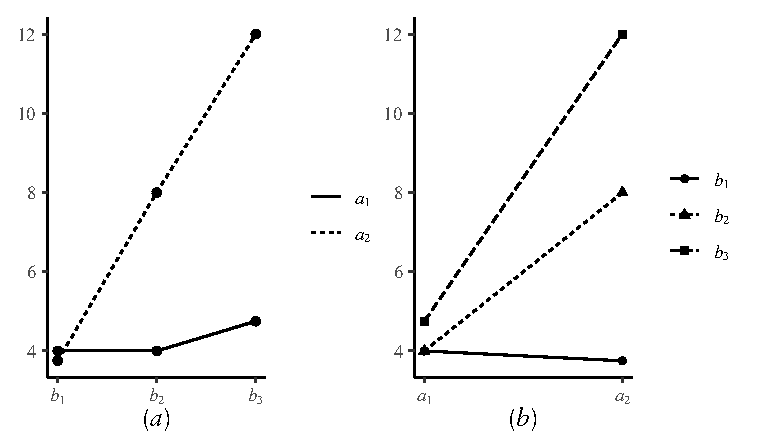
\includegraphics{cross_effect_two_directions}
    \caption{$AB$交互作用两个方向的图}
    \labfig{AB_cross_two_directions}
\end{figure}



对两个图的解释是不一样的,\reffig{AB_cross_two_directions}(a)表明,$B$因素在$A$因素的两个水平上影响趋势是不一致的.$B$因素的三个水平在$a_1$水平似乎没有明显差别,而在$a_2$水平有较大差异.
\reffig{AB_cross_two_directions}(b)表明,$A$因素在$B$因素的三个水平上的影响趋势也不一致.$A$因素的两个水平在$b_1$水平没有明显差异,而在$b_2,b_3$水平存在较大差异.

图解法的优点是简单、直观.直接利用各处理水平结合所得的平均观测值作图,可以使读者对结果模式有一个非常直观的了解.它的弱点是,解释是主观的,有时不同的研究者可能会对同一结果作出不同的解释,尤其是当出现复杂的交互作用时,研究者单靠经验、直观进行解释是很困难的.因此,图解一般只能作为检查交互作用的第一步,它需要同统计检验结合起来,以便进一步用数据对交互作用的意义作出更精确可靠的解释.

\subsection{简单效应检验}
\subsubsection{基本特点}

检查交互作用含义的另一个方法是简单效应检验,简单效应检验与主效应检验不大相同.主效应检验是在忽略其它因素的情况下检验一个因素的处理效应,我们比较一下主效应和简单效应的不同之处.

设观测值为$Y_{ijk}$,$i$是处理组合内的第$i$个被试,$j$是因素$A$的的水平$j$,$k$是因素$B$的水平$k$

1. $A$因素和$B$因素的\textbf{主效应}用组内平均数与真值的差估计,组内平均数忽略了被试和其它因素,可表示为
\[ \begin{array}{cc}
    \alpha _1 = \mu _{.1.} - \mu    &    \beta _1 = \mu _{..1} - \mu\\ 
    \alpha _2 = \mu _{.2.} - \mu    &    \beta _2 = \mu _{..2} - \mu\\
    \vdots                          &     \vdots \\
    \alpha _j = \mu _{.j.} - \mu    &    \beta _k = \mu _{..k} - \mu\\
    
    \alpha _p = \mu _{.p.} - \mu    &    \beta _q = \mu _{..q} - \mu
\end{array}\]

可检验的假说是:

(1)$A$因素处理水平上的总体平均数相等,即:
\[H_0 : \mu _{.1.} = \mu _{.2.} = \cdots = \mu _{.p.}\]

或$A$因素处理效应为0,即:
\[ \alpha _j = 0 \]

(2)$B$因素处理水平上的总体平均数相等,即:
\[ H_0 : \mu _{..1} = \mu _{..2} = \cdots = \mu _{..q} \]

或$B$因素处理效应为0,即:
\[ \beta _k =0 \]

2.\textbf{简单效应}

%这段话没写好

本例中,对于因素$A$,我们分别计算它的效应在$b_1,b_2,b_3$上的变异,
\reffig{AB_cross_two_directions}(b)上三条线段因为斜率不一样所以我们怀疑可能存在交互作用,而上述拆分的三个变异的显著性正好反应这条线在统计上是显著的平还是显著的斜
如果$A$在$b1$上的变异不显著,而在$b_2,b_3$上的变异显著,则说明确实存在交互作用.

所以说简单效应的计算也就是将一个因素对因变量的效应拆分成多组,有另一个因素有多少水平就拆分成多少个组,我们检验它在另一个因素不同水平上的显著性.

\[\begin{array}{cc}
    \alpha _{1\left( \text{在}b_1\text{水平上} \right)} = \mu _{.11} - \mu _{..1} & \beta _{1\left( \text{在}a_1\text{水平上} \right)} = \mu _{.11} - \mu _{.1.}\\
    \alpha _{2\left( \text{在}b_1\text{水平上} \right)} = \mu _{.21} - \mu _{..1}& \beta _{2\left( \text{在}a_1\text{水平上} \right)} = \mu _{.12} - \mu _{.2.}\\
    \vdots                                              & \vdots\\
    \alpha _{j\left( \text{在}b_1\text{水平上} \right)} = \mu _{.j1} - \mu _{..1}&\beta _{k\left( \text{在}a_1\text{水平上} \right)}= \mu _{.1k} - \mu _{.1.}\\
    \vdots                                              & \vdots\\
    \alpha _{j\left( \text{在}b_k\text{水平上} \right)} = \mu _{.jk} - \mu _{..k}& \beta _{k\left( \text{在}a_j\text{水平上} \right)}= \mu _{.jk} - \mu _{j.}\\
    \vdots                                              & \vdots\\
    \alpha _{p\left( \text{在}b_q\text{水平上} \right)} = \mu _{.pq} - \mu _{..q}& \beta _{q\left( \text{在}a_p\text{水平上} \right)}= \mu _{.pq} - \mu _{.p.}
\end{array}\]




\subsubsection{计算举例}


\subsubsection{使用}
%------------------------------------两因素随机区组实验设计
\section{两因素随机机区组实验设计}




%\setchapterpreamble[u]{\margintoc}
\chapter{两因素重复测量实验设计}
\labch{options}


\subsection{基本特点}

\begin{margintable}
  \centering
  \caption{Add caption}
    \begin{math}    
        \begin{array}{cccc}
        \toprule
               & b_1 & b_2 & b_3\\
        \midrule
        \multirow{4}[0]{*}{$a_1$} & S_1    & S_1    & S_1 \\
               & S_2    & S_2    & S_2 \\
               & S_3    & S_3    & S_3 \\
               & S_4    & S_4    & S_4 \\
        \midrule
        \multirow{4}[0]{*}{$a_2$} & S_5    & S_5    & S_5 \\
               & S_6    & S_6    & S_6 \\
               & S_7    & S_7    & S_7 \\
               & S_8    & S_8    & S_8 \\
        \bottomrule
        \end{array}
    \end{math}
  \label{tab:addlabel}
\end{margintable}

\subsubsection{两因素混合实验设计模型}

\begin{definition}[两因素混合实验设计模型]
\labdef{two_way_mixed_model}

\begin{align*}
    Y_{ijk} = \mu + \alpha _j + \pi _{i \left( j \right)} + \beta _k + \left( \alpha \beta \right) _{jk} +  \left( \beta \pi \right) _{ki \left( j \right)} + \varepsilon _{ijk}\\
    \left( j=1,2,\cdots ,p; k=1,2,\cdots,q; i=1,2,\cdots,n \right)
\end{align*}

其中

\begin{tabular}{lcl}
    $\mu$                                              & - & 总体平均数,或真值\\
    $\alpha _j$                                        & - & $A$因素的水平$j$的处理效应\\
    $\pi _{i \left( j \right)}$                        & - & 嵌套在$\alpha _j$水平内的被试$i$的效应\\
    $\beta _k$                                         & - & $B$因素的水平$k$的处理效应\\
    $\left( \alpha \beta \right) _{jk}$                & - & 水平$\alpha _j$和水平$\beta _k$的交互作用\\
    $\left( \beta \pi \right) _{ki \left( j \right) }$ & - & 嵌套在$\beta _k$水平和被试$i$的交互作用的残差\\
    $\varepsilon _{ijk}$                               & - & 误差\\
\end{tabular}

\end{definition}

\subsubsection{两因素混合实验设计检验的假说}

\subsection{实验设计与计算举例}
\subsubsection{研究的问题}

\textbf{1.计算表}

\textbf{2.各种基本量的计算}

\textbf{3.平方和分解与计算}
\begin{definition}[两因素混合实验设计平方和分解]
\labdef{two_way_mixed_variance}
\begin{alignat*}{3}
    &  SS_{\text{总变异}}    &&=    SS_{\text{被试间}} &&+    SS_{\text{被试内}} \\
    &                       &&=    \left( SSA + SS_{\text{被试} \left( A \right) } \right)  &&+    \left( SSB + SSAB + SS_{B\times \text{被试} \left( A \right) } \right)
\end{alignat*}
\end{definition}

\begin{alignat*}{4}
    &  SS_{\text{总变异}}    &&=    [ABS] - [Y]    &&=    251.833\\
    &  SS_{\text{被试间}}    &&=    [AS]  - [Y]    &&=    111.166\\
    &  SSA                   &&=    [A]   - [Y]   &&=    80.667\\
    &  SS_{\text{被试}\left( A \right)}    &&=    SS_{\text{被试间}} - SSA     &&= 30.500\\
    &  SS_{\text{被试内}}    &&=    SS_{\text{总变异}} - SS_{\text{被试间}}    &&= 140.667\\
    &  SSB                   &&=    [B] - [Y]     &&=    81.083\\
    &  SSAB                  &&=    [AB]- [Y] -SSA -SSB     &&=56.584\\
    &  SS_{B \times \text{被试} \left( A \right)}    &&=    SS_{\text{被试内}} - SSB - SSAB    &&=    3.000
\end{alignat*}

\textbf{4.方差分析表及结果的解释}

\begin{table*}
	\centering
	\caption{两因素混合实验设计方差分析表}
	\label{two_way_mixed_ANOVA_tab}
	{
                    \begin{tabular}{lrrrrrr}
		    \toprule
			\multicolumn{1}{c}{变异源} & \multicolumn{1}{c}{$SS$} & \multicolumn{1}{c}{$df$} & \multicolumn{1}{c}{$MS$} & \multicolumn{1}{c}{$F$} & \multicolumn{1}{c}{$p$} \\
		    \midrule
		    	$A$(主题熟悉性) & 80.667 & $p-1=1$ & 80.667 & 15.869 & 0.007  \\
			被试间($A$) & 30.500 & $p(n-1)=6$ & 5.083 &  &    \\
		    \midrule
			$B$(生字密度) & 81.083 & $q-1=2$ & 40.542 & 162.167 & $<$ .001  \\
			$AB$ & 56.583 & $(p-1)(q-1)=2$ & 28.292 & 113.167 & $<$ .001  \\
			$B\times$被试$(A)$ & 3.000 & $p(n-1)(q-1)=12$ & 0.250 &  &    \\
		    \bottomrule
		\end{tabular}
	}
\end{table*}

\textbf{5.平方和与自由度分解图}

\subsection{一些解释}
\textbf{1.各种平方和的意义}


\textbf{2.$SS_{\text{被试}\left( A \right)}$的实质}

忽略$B$因素,将其各个水平的值求和,得到\reftab{two_way_omit_B_AS_tab}的计算表,观察这个表的被试分配到处理的模式可以看到,因素$A$的两个水平下,$a_1$水平下有4个被试,每个被度仅接受一种处理;$a_1$水平下有4个被试,每个被度仅接受一种处理.这样就好像是一个单因素完全随机设计.接下来我们计算这个完全随机设计的单元内误差,注意算的时候要忘记$B$当成完全随机,但是被试数要带上$B$因素的被试数,否则平方和会拉大.

(1)基本量的计算

\begin{margintable}
  \centering
  \caption{忽略$B$因素(被试内变量)的$AS$表}
    \[\begin{array}{crr}
        \toprule
              & \multicolumn{1}{c}{a_1}   & \multicolumn{1}{c}{a_2} \\
        \midrule
              & \multicolumn{1}{l}{n=3} &  \\
              & S_1=12 & S_5=24 \\
              & S_2=19 & S_6=27 \\
              & S_3=13 & S_7=23 \\
              & S_4=7 & S_8=21 \\
        \midrule
            \sum  & \multicolumn{1}{c}{51}    & \multicolumn{1}{c}{95} \\
        \bottomrule
    \end{array}\]
  \labtab{two_way_omit_B_AS_tab}
\end{margintable}

\begin{alignat*}{3}
    &\left[ Y \right]  &&=  \frac{\left( 146 \right) ^2}{24}                                         &&=888.167\\
    &\left[ AS \right] &&=  \frac{\left( 12 \right) ^2}{3}+\frac{\left( 19 \right) ^2}{3}+\cdots     &&=999.333\\
    &\left[ A \right]  && = \frac{\left( 51 \right) ^2}{12}+\frac{\left( 95 \right) ^2}{12}          &&=968.833
\end{alignat*}

(2)平方和的计算
\begin{alignat*}{3}
    & SS_{\text{总变异}} &&=     [AS] - [Y]                             &&= 111.166\\
    & SS_{\text{组间}}   &&=     [A] - [Y]                              &&= 80.667\\
    & SS_{\text{组内}}   &&=     SS_{\text{总变异}} - SS_{\text{组间}}  &&= 30.500
\end{alignat*}

所以在混合因素设计中的
\[ F=\frac{MSA}{MS_{\text{被试}\left( A \right)}}=\frac{SSA/\left( p-1 \right)}{SS_{\text{被试}\left( A \right)}/\left( n-1 \right) p} \]

类似于完全随机设计中的

\[ F=\frac{MS_{\text{组间}}}{MS_{\text{组内}}}=\frac{SS_{\text{组间}}/\left( p-1 \right)}{SS_{\text{组内}}/p\left( n-1 \right)} \]

上面$SS_{\text{组内}}$是用相减法算得,因其实质是单元内误差,也可以直接计算,其算法我们也已知晓,即每个处理内的被试间的变异.

\begin{alignat*}{3}
    &    SS_{\text{1组}}    &&=    \frac{\left( 12 \right) ^2}{3}+\frac{\left( 19 \right) ^2}{3}+\frac{\left( 13 \right) ^2}{3}+\frac{\left( 7 \right) ^2}{3}-\frac{\left( 51 \right) ^2}{12}    &&=    24.25\\
    &    SS_{\text{2组}}    &&=    \frac{\left( 24 \right) ^2}{3}+\frac{\left( 27 \right) ^2}{3}+\frac{\left( 23 \right) ^2}{3}+\frac{\left( 21 \right) ^2}{3}-\frac{\left( 95 \right) ^2}{12}    &&=    6.25\\
    &    SS_{\text{组内}}    &&=24.25+6.25                                    &&=    30.5
\end{alignat*}

\textbf{3.$SS_{B\times \text{被试}\left( A \right)}$的实质}



\begin{margintable}
  \centering
  \caption{在$a_1$水平的$BS$表}
    \begin{tabular}{ccccc}
          & $b_1$ & $b_2$ & $b_3$ & $\sum$ \\
    $S_1$ & \cellcolor[rgb]{ .886,  .937,  .855}3 & \cellcolor[rgb]{ .886,  .937,  .855}4 & \cellcolor[rgb]{ .886,  .937,  .855}5 & \cellcolor[rgb]{ 1,  .949,  .8}12 \\
    $S_2$ & \cellcolor[rgb]{ .886,  .937,  .855}6 & \cellcolor[rgb]{ .886,  .937,  .855}6 & \cellcolor[rgb]{ .886,  .937,  .855}7 & \cellcolor[rgb]{ 1,  .949,  .8}19 \\
    $S_3$ & \cellcolor[rgb]{ .886,  .937,  .855}4 & \cellcolor[rgb]{ .886,  .937,  .855}4 & \cellcolor[rgb]{ .886,  .937,  .855}5 & \cellcolor[rgb]{ 1,  .949,  .8}13 \\
    $S_4$ & \cellcolor[rgb]{ .886,  .937,  .855}3 & \cellcolor[rgb]{ .886,  .937,  .855}2 & \cellcolor[rgb]{ .886,  .937,  .855}2 & \cellcolor[rgb]{ 1,  .949,  .8}7 \\
    $\sum$ & \cellcolor[rgb]{ .929,  .929,  .929}16 & \cellcolor[rgb]{ .929,  .929,  .929}16 & \cellcolor[rgb]{ .929,  .929,  .929}19 & \cellcolor[rgb]{ .867,  .922,  .969}51 \\
    \end{tabular}%
  \labtab{two_way_mixed_a1}
\end{margintable}



\begin{alignat*}{3}
    &    \colorbox[rgb]{ .867,  .922,  .969}{$[Y_1]$}
    &&   =\frac{\left( 51 \right) ^2}{12}
    &&   =216.75\\
    &    \colorbox[rgb]{ .886,  .937,  .855}{$[B_1S_1]$}
    &&   = \left( 3 \right) ^2+\left( 4 \right) ^2+\cdots 
    &&   =245.000\\
    &    \colorbox[rgb]{ 1,  .949,  .8}{$[S_1]$}
    &&   =\frac{\left( 12 \right) ^2}{3}+\frac{\left( 19 \right) ^2}{3}+\frac{\left( 13 \right) ^2}{3}+\frac{\left( 7 \right) ^2}{3}
    &&   =241\\
    &    \colorbox[rgb]{ .929,  .929,  .929}{$[B_1]$}
    &&   = \frac{\left( 16 \right) ^2}{4}+\frac{\left( 16 \right) ^2}{4}+\frac{\left( 19 \right) ^2}{4}
    &&   = 218.25
\end{alignat*}




\begin{alignat*}{3}
    &    \colorbox[rgb]{ .867,  .922,  .969}{$[Y_2]$}
    &&   =\frac{\left( 95 \right) ^2}{12}
    &&   =752.803\\
    &    \colorbox[rgb]{ .886,  .937,  .855}{$[B_2S_2]$}
    &&   = \left( 4 \right) ^2+\left( 8 \right) ^2+\cdots 
    &&   =888.250\\
    &    \colorbox[rgb]{ 1,  .949,  .8}{$[S_2]$}
    &&   =\frac{\left( 24 \right) ^2}{3}+\frac{\left( 27 \right) ^2}{3}+\frac{\left( 23 \right) ^2}{3}+\frac{\left( 21 \right) ^2}{3}
    &&   =758.333\\
    &    \colorbox[rgb]{ .929,  .929,  .929}{$[B_2]$}
    &&   = \frac{\left( 15 \right) ^2}{4}+\frac{\left( 32 \right) ^2}{4}+\frac{\left( 48 \right) ^2}{4}
    &&   = 888.25
\end{alignat*}

\begin{alignat*}{3}
    & SS_{总_1}
    &&=\left[ B_1S_1 \right] -\left[ Y_1 \right] 
    &&=28.25\\
    & SSB_1
    &&=\left[ B_1 \right] -\left[ Y_1 \right] 
    &&=1.5\\
    & SS_{\text{被试}_1}
    &&=\left[ S_1 \right] -\left[ Y_1 \right] 
    &&=24.25\\
    & SS\left( B_1S_1 \right) 
    &&=\left[ B_1S_1 \right] -\left[ Y_1 \right] -SSB_1-SS_{\text{被试}_1}
    &&=2.5 
\end{alignat*}
\begin{alignat*}{3}
    & SS_{总_2}
    &&=\left[ B_2S_2 \right] -\left[ Y_2 \right] 
    &&=142.917\\
    & SSB_2
    &&=\left[ B_2 \right] -\left[ Y_2 \right] 
    &&=136.167\\
    & SS_{\text{被试}_2}
    &&=\left[ S_2 \right] -\left[ Y_2 \right] 
    &&=6.25\\
    & SS\left( B_2S_2 \right) 
    &&=\left[ B_2S_2 \right] -\left[ Y_2 \right] -SSB_2-SS_{\text{被试}_2}
    &&=0.5
\end{alignat*}

然后合并两个残差

\begin{align*}
    MS_{\text{残差} \left( pooled\right) } &= \frac{SSB_1S_1+SSB_2S_2}{(n-1)(q-1)+(n-1)(q-1)}\\
                                           &= \frac{2.5+0.5}{12}\\
                                           &= 0.25
\end{align*}

\begin{margintable}
  \centering
  \caption{在$a_2$水平的$BS$表}
    \begin{tabular}{ccccc}
          & $b_1$ & $b_2$ & $b_3$ & $\sum$ \\
    $S_5$ & \cellcolor[rgb]{ .886,  .937,  .855}4 & \cellcolor[rgb]{ .886,  .937,  .855}8 & \cellcolor[rgb]{ .886,  .937,  .855}12 & \cellcolor[rgb]{ 1,  .949,  .8}24 \\
    $S_6$ & \cellcolor[rgb]{ .886,  .937,  .855}5 & \cellcolor[rgb]{ .886,  .937,  .855}9 & \cellcolor[rgb]{ .886,  .937,  .855}13 & \cellcolor[rgb]{ 1,  .949,  .8}27 \\
    $S_7$ & \cellcolor[rgb]{ .886,  .937,  .855}3 & \cellcolor[rgb]{ .886,  .937,  .855}8 & \cellcolor[rgb]{ .886,  .937,  .855}12 & \cellcolor[rgb]{ 1,  .949,  .8}23 \\
    $S_8$ & \cellcolor[rgb]{ .886,  .937,  .855}3 & \cellcolor[rgb]{ .886,  .937,  .855}7 & \cellcolor[rgb]{ .886,  .937,  .855}11 & \cellcolor[rgb]{ 1,  .949,  .8}21 \\
    $\sum$ & \cellcolor[rgb]{ .929,  .929,  .929}15 & \cellcolor[rgb]{ .929,  .929,  .929}32 & \cellcolor[rgb]{ .929,  .929,  .929}48 & \cellcolor[rgb]{ .867,  .922,  .969}95 \\
    \end{tabular}
  \labtab{two_way_mixed_a2}
\end{margintable}

\subsection{基本特点}

\begin{margintable}
  \centering
  \caption{Add caption}
    $\begin{array}{cccccc}
    \toprule
        a_1    & a_1    & a_1    & a_2    & a_2    & a_2 \\
        b_1    & b_2    & b_3    & b_1    & b_2    & b_3 \\
    \midrule
        S_1    & S_1    & S_1    & S_1    & S_1    & S_1 \\
        S_2    & S_2    & S_2    & S_2    & S_2    & S_2 \\
        S_3    & S_3    & S_3    & S_3    & S_3    & S_3 \\
        S_4    & S_4    & S_4    & S_4    & S_4    & S_4 \\
    \bottomrule
    \end{array}$
  \label{tab:addlabel}%
\end{margintable}%

\subsubsection{两因素被试内实验设计模型}

\begin{definition}[两因素被试内实验设计模型]
\labdef{two_way_within_model}

\begin{align*}
 Y_{ijk}=\mu +\alpha _j+\left( \alpha \pi \right) _{ji}+\beta _k+\left( \beta \pi \right) _{ki}+\left( \alpha \beta \right) _{jk}+\left( \alpha \beta \pi \right) _{jki}+\varepsilon _{ijk}\\
\left( j=1,2,\cdots ,p;k=1,2,\cdots ,q;i=1,2,\cdots ,n \right) 
\end{align*}

其中

\begin{tabular}{lcl}
    $\mu$                                        & - &    总体平均数或真值\\
    $\pi _i$                                     & - &    由被试$i$引起的变异,被试间变异\\
    $\alpha _j$                                  & - &    $A$因素的水平$j$引起的处理效应\\
    $\left( \alpha \pi \right) _{ji}$            & - &    水平$\alpha _j$和被试$i$的交互作用\\
    $\beta _k$                                   & - &    $B$因素的水平$k$引起的处理效应\\
    $\left( \beta \pi \right) _{ki}$             & - &    水平$\beta _k$和被试$i$的交互作用\\
    $\left( \alpha \beta \right) _{jk}$          & - &    水平$\alpha _j$和水平$\beta _k$的交互作用\\
    $\left( \alpha \beta \pi \right) _{jki}$     & - &    水平$\alpha _j, \beta _k$和被试$i$的交互作用\\
\end{tabular}

\end{definition}

\subsubsection{两因素被试内实验设计检验的假说}

\subsection{实验设计与计算举例}
\subsubsection{研究的问题}

\textbf{1.计算表}

\textbf{2.各种基本量的计算}

\textbf{3.平方和分解与计算}
\begin{definition}[两因素被试内实验设计平方和分解]
\labdef{two_way_within_variance}
\begin{alignat*}{3}
    &  SS_{\text{总变异}} &&= SS_{\text{被试间}} &&+ SS_{\text{被试内}}\\ 
    &                     &&= SS_{\text{被试间}} &&+ \left( SSA+SS_{A\times \text{被试}}+SSB+SS_{B\times \text{被试}}+SSAB+SS_{A\times B\times \text{被试}} \right) 
\end{alignat*}
\end{definition}

\begin{alignat*}{3}
    &  SS_{\text{总变异}}                               &&=    [ABS] - [Y] &&= 251.833                                                                                    \\
    &  SS_{\text{被试间}}                               &&=    [S]-[Y]     &&= 27.167                                                                                     \\
    &  SS_{\text{被试内}}                               &&=    SS_{\text{总变异}} - SS_{\text{被试间}} &&= 224.667                                                         \\
    &  SSA                                              &&=    [A] - [Y] &&= 80.667                                                                                       \\
    &  SS_{A \times \left( \text{被试} \right)}         &&=    [AS] - [Y] - SSA - SS_{\text{被试间}} &&= 3.333                                                             \\
    &  SSB                                              &&=    [B]  - [Y] &&= 81.083                                                                                      \\
    &  SS_{B \times \left( \text{被试} \right)}         &&=    [BS] - [Y] - SSB - SS_{\text{被试间}} &&= 1.583                                                             \\
    &  SSAB                                             &&=    [AB] - [Y] - SSA - SSB &&= 56.583                                                                          \\
    &  SS_{A \times B \times \text{被试}}               &&=    SS_{\text{被试内}} - SSA - SS_{A \times \text{被试}} - SSB - SS_{B\times \text{被试}} - SSAB &&= 1.417 
\end{alignat*}

\textbf{4.方差分析表及结果的解释}
\begin{table*}
	\centering
	\caption{两因素被试内实验设计方差分析表}
	\labtab{two_way_ANOVA_tab}
	{
                    \begin{tabular}{lrrrrrr}
		    \toprule
			\multicolumn{1}{c}{变异源} & \multicolumn{1}{c}{$SS$} & \multicolumn{1}{c}{$df$} & \multicolumn{1}{c}{$MS$} & \multicolumn{1}{c}{$F$} & \multicolumn{1}{c}{$p$} \\
		     \midrule
			被试间                 & 27.167    & $n-1=3$     &     &  &    \\
		      \midrule
			$A$(主题熟悉性)        & 80.667    & $p-1=1$     & 80.667  & 72.600 & 0.003  \\
			$A\times$被试          & 3.333     & $(p-1)(n-1)=3$     & 1.111   &  &    \\
			$B$                    & 81.083    & $q-1=2$     & 40.542 & 153.632 & $<$ .001  \\
			$B\times$被试          & 1.583     & $(n-1)(q-1)=6$     & 0.264   &  &    \\
			$A \times B$           & 56.583    & $(p-1)(q-1)=2$     & 28.292  & 119.824 & $<$ .001  \\
			$A\times B \times$被试 & 1.417     & $(n-1)(p-1)(q-1)=6$     & 0.236   &  &    \\
		      \bottomrule
		\end{tabular}
	}
\end{table*}


\textbf{5.平方和与自由度分解图}

\subsection{一些解释}
\textbf{1.各种平方和的意义}




%\setchapterpreamble[u]{\margintoc}
\chapter{三因素被试间实验设计}
\labch{options}
%\setchapterpreamble[u]{\margintoc}
\chapter{三因素重复测量实验设计}
\labch{options}

%----------------------------------------------------------------------------------------

\backmatter % Denotes the end of the main document content

\setchapterstyle{plain} % Output plain chapters from this point onwards

%----------------------------------------------------------------------------------------
%	BIBLIOGRAPHY
%----------------------------------------------------------------------------------------

% The bibliography needs to be compiled on the command line with 'biber main' from the template directory

\defbibnote{bibnote}{Here are the references in citation order.\par\bigskip} % Prepend this text to the bibliography
\printbibliography[heading=bibintoc, title=参考文献, prenote=bibnote] % Add the bibliography heading to the ToC and set the title of the bibliography

%----------------------------------------------------------------------------------------
%	NOMENCLATURE
%----------------------------------------------------------------------------------------

% The nomenclature needs to be compiled on the command line with 'makeindex main.nlo -s nomencl.ist -o main.nls' from the template directory

\nomenclature{$c$}{Speed of light in a vacuum inertial frame}
\nomenclature{$h$}{Planck constant}

\renewcommand{\nomname}{Notation}
\renewcommand{\nompreamble}{The next list describes several symbols that will be later used within the body of the document.}
\printnomenclature % Output the nomenclature

%----------------------------------------------------------------------------------------
%	GREEK ALPHABET
% 	Originally from https://gitlab.com/jim.hefferon/linear-algebra
%----------------------------------------------------------------------------------------

\vspace{3cm}
{\usekomafont{chapter}Greek letters with pronounciation} \\[2ex]
\begin{center}
	\newcommand{\pronounced}[1]{\hspace*{.2em}\small\textit{#1}}
	\begin{tabular}{l l @{\hspace*{3em}} l l}
		\toprule
		Character & Name & Character & Name \\ 
		\midrule
		$\alpha$ & alpha \pronounced{AL-fuh} & $\nu$ & nu \pronounced{NEW} \\
		$\beta$ & beta \pronounced{BAY-tuh} & $\xi$, $\Xi$ & xi \pronounced{KSIGH} \\ 
		$\gamma$, $\Gamma$ & gamma \pronounced{GAM-muh} & o & omicron \pronounced{OM-uh-CRON} \\
		$\delta$, $\Delta$ & delta \pronounced{DEL-tuh} & $\pi$, $\Pi$ & pi \pronounced{PIE} \\
		$\epsilon$ & epsilon \pronounced{EP-suh-lon} & $\rho$ & rho \pronounced{ROW} \\
		$\zeta$ & zeta \pronounced{ZAY-tuh} & $\sigma$, $\Sigma$ & sigma \pronounced{SIG-muh} \\
		$\eta$ & eta \pronounced{AY-tuh} & $\tau$ & tau \pronounced{TOW (as in cow)} \\
		$\theta$, $\Theta$ & theta \pronounced{THAY-tuh} & $\upsilon$, $\Upsilon$ & upsilon \pronounced{OOP-suh-LON} \\
		$\iota$ & iota \pronounced{eye-OH-tuh} & $\phi$, $\Phi$ & phi \pronounced{FEE, or FI (as in hi)} \\
		$\kappa$ & kappa \pronounced{KAP-uh} & $\chi$ & chi \pronounced{KI (as in hi)} \\
		$\lambda$, $\Lambda$ & lambda \pronounced{LAM-duh} & $\psi$, $\Psi$ & psi \pronounced{SIGH, or PSIGH} \\
		$\mu$ & mu \pronounced{MEW} & $\omega$, $\Omega$ & omega \pronounced{oh-MAY-guh} \\
		\bottomrule
	\end{tabular} \\[1.5ex]
	Capitals shown are the ones that differ from Roman capitals.
\end{center}

%----------------------------------------------------------------------------------------
%	GLOSSARY
%----------------------------------------------------------------------------------------

% The glossary needs to be compiled on the command line with 'makeglossaries main' from the template directory

\newglossaryentry{computer}{
	name=computer,
	description={is a programmable machine that receives input, stores and manipulates data, and provides output in a useful format}
}

\newacronym[longplural={Frames per Second}]{fpsLabel}{FPS}{Frame per Second}
\newacronym[longplural={Tables of Contents}]{tocLabel}{TOC}{Table of Contents}

\setglossarystyle{listgroup} % Set the style of the glossary (see https://en.wikibooks.org/wiki/LaTeX/Glossary for a reference)
\printglossary[title=Special Terms, toctitle=List of terms] % Output the glossary, 'title'  is the chapter heading for the glossary, toctitle is the table of contents heading

%----------------------------------------------------------------------------------------
%	INDEX
%----------------------------------------------------------------------------------------

% The index needs to be compiled on the command line with 'makeindex main' from the template directory

\printindex % Output the index

%----------------------------------------------------------------------------------------
%	BACK COVER
%----------------------------------------------------------------------------------------

% If you have a PDF file that you want to use as back cover, uncomment the following lines.

%\clearpage
%\thispagestyle{empty}
%\null%
%\clearpage
%\includepdf{cover-back.pdf}

%----------------------------------------------------------------------------------------

\end{document}